\documentclass{article}
\usepackage{mystyle}

\title{Lectures in Polytopes}
\author{Answers (unofficial)}

\begin{document}

\maketitle
\tableofcontents

\begin{figure}[H]
    \centering

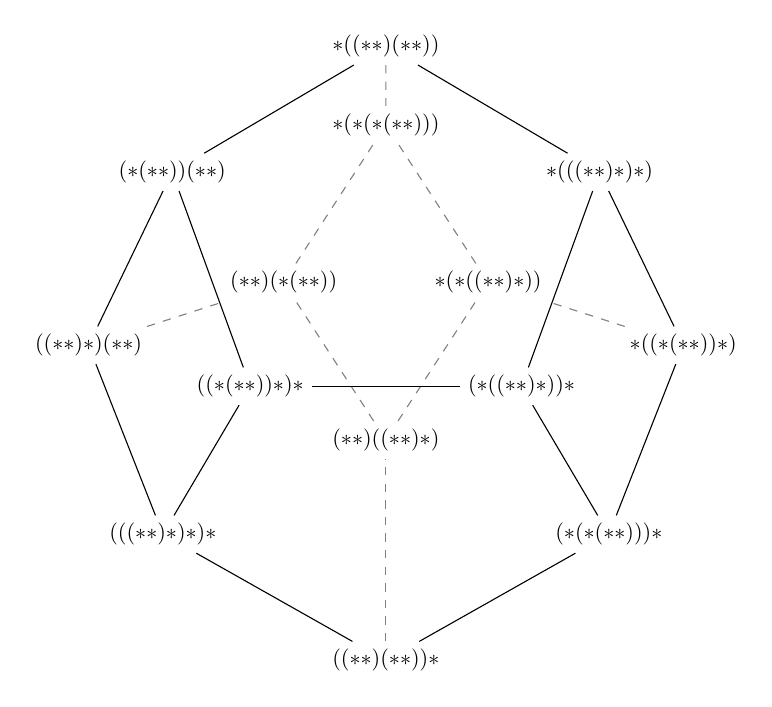
\begin{tikzpicture}[x=1.18mm,y=1mm,scale=2,>=stealth]
  \tikzset{every node/.style={scale=.8}}
  
  \node (1120) at (-7.3,-1.6)  {$((\ast(\ast\ast))\ast)\ast$};
  \node (1210) at ( 7.3,-1.6)  {$(\ast((\ast\ast)\ast))\ast$};
  \node (3010) at ( 0, 20)     {$\ast((\ast\ast)(\ast\ast))$};
  \node (1201) at ( 0,-19)     {$((\ast\ast)(\ast\ast))\ast$};
  \node (2011) at (-16, 1)     {$((\ast\ast)\ast)(\ast\ast)$};
  \node (2200) at ( 16, 1)     {$\ast((\ast(\ast\ast))\ast)$};
  \node (2020) at (-11.5,12)   {$(\ast(\ast\ast))(\ast\ast)$};
  \node (2110) at ( 11.5,12)   {$\ast(((\ast\ast)\ast)\ast)$};
  \node (1111) at (-12,-11)    {$(((\ast\ast)\ast)\ast)\ast$};
  \node (1300) at ( 12,-11)    {$(\ast(\ast(\ast\ast)))\ast$};
  \node (4000) at ( 0, 15)     {$\ast(\ast(\ast(\ast\ast)))$};
  \node (2101) at ( 0, -5)     {$(\ast\ast)((\ast\ast)\ast)$};
  \node (3001) at (-5.5, 5)    {$(\ast\ast)(\ast(\ast\ast))$};
  \node (3100) at ( 5.5, 5)    {$\ast(\ast((\ast\ast)\ast))$};

  \path[-,dashed,color=black!50!white]
    (2011) edge (3001)
    (2200) edge (3100)
    (1201) edge (2101)
    (3010) edge (4000)
    (2101) edge (3001)
    (3001) edge (4000)
    (2101) edge (3100)
    (3100) edge (4000);

  \path[-]
    (1120) edge (1210)
    (1210) edge (2110)
    (2110) edge (3010)
    (1120) edge (2020)
    (2020) edge (3010)
    (1210) edge (1300)
    (1111) edge (1120)
    (1111) edge (1201)
    (1201) edge (1300)
    (1111) edge (2011)
    (2011) edge (2020)
    (1300) edge (2200)
    (2110) edge (2200);
\end{tikzpicture}

\caption{The Associahedron $K_3$}
\end{figure}

\pagebreak

This is a solutions set on G.M Ziegler's \textit{Lectures on Polytopes} \cite{ziegler-lectures-polytopes}. We acknowledge the abundance of errors and unclear writing, and this is also a work in progress; please contact EXmasterpiece on discord or email yuchennnxu@gmail.com for corrections, suggestions, clarifications, or discussions.

\bigskip
A few words on the writing: Most of the notation follows notation convention from Ziegler: here are important/different ones

\smallskip
$\boxplus$ denotes the Minkowski sum,

$[x,y]$ denotes the line segment from $x$ to $y$,

$\textbf{0}$ denotes the column zero vector,

$\mathds{O}$ denotes the row zero vector,

$2^A$ for a set $A$ means the power set $\mathcal{P}(A)$, so $\mathcal{S} \subseteq 2^A$ means it is a set of subsets of $A$.

$\sqcup$ denotes the disjoint union.

$[n]$ denotes the set $\{1, 2, \ldots n\}$.

Sometimes we will write something like $abcd$ (a concatenated string) to mean the set $\{a,b,c,d\}$. If we do, the context shall always make it clear that the $abcd$ is intended as a set, not a number.

$\binom{n}{k}$ continues to denote the binomial coefficient, and we will write $\binom{[n]}{k}$ to mean all the size $k$ subsets of $[n]$.

Certain diagrams and figures will be ommitted. I will put a picture only if it absolutely central to the exercise, but otherwise refer to Ziegler  \cite{ziegler-lectures-polytopes} for the illustrations. We attest they are quite helpful. Similarly, refer to Ziegler for the references \& citations; the bracketed numbers (as citation) have been kept but the sources will not be in the bibliography. Unfortunately no progress is made on the unsolved problems.

Let us begin!

\setcounter{section}{-1}
\bigskip
\section{Introduction \& Examples}
\begin{enumerate}
\setcounter{enumi}{-1}
\renewcommand{\labelenumi}{0.\arabic{enumi}}

\item Given a $3$-dimensional polytope such that every two vertices are
adjacent, show that it is a tetrahedron.

\begin{proof} 
    Clearly there must be $\geq 4$ vertices for the polytope to be non-planar, and if there are exactly $4$ vertices we just have a tetrahedron. If $v > 4$ and $e = \binom{v}{2}$, by Euler's formula we get
\[f = 2+\binom{v}{2}-v \]
but also, since each edge is in exactly $2$ faces, and each face has at minimum $3$ edges

\[f \leq \frac{2e}{3} = \frac{2\binom{v}{2}}{3}\]

But since $v \geq 5$, $\binom{v}{2} \geq 10$, and yet we have

\[v-2 \geq \frac{1}{3}\binom{v}{2}, \quad 5-2 \geq \frac{10}{3}\]

Which is a contradiction, since $\binom{v}{2} = \frac{v(v+1)}{2}$ grows faster than $v$.
\end{proof}


\item Show that if a polytope is both simple and simplicial, then it is a simplex or an $n$-gon.

\smallskip
Similarly, if a $d$-polytope is simple and \emph{cubical} (i.e., all its facets are
combinatorially equivalent to $(d-1)$-cubes, then $P$ is a $d$-cube or an
$n$-gon.

\begin{proof}
    If a polytope of dimension $d$ is \textit{simple}, each vertex is contained in exactly $d$ edges. If it is \textit{simplicial}, each facet must be a minimal. First consider $d = 2$. Then the minimal facets are the $1$ dimensional edges, and since $\deg(v) = 2$ we see these are exactly the $n$-gons. 
    
    Now let $d > 2$ and the minimal facets are exactly the $d-1$ dimensional simplexes. Consider a facet $f$ and a vertex $v_i$ in the facet. Since the polytope is simple, $v_i$ has at most one more edge outside of $f$, which connects $v_i$ to $v$, say. Since the polytope is simplicial, every facet is a simplex, which further means that every k-face is a k-simplex. So, the 2-face containing the edges $(v_i, v)$ and $(v_i, v_j)$ must be a triangle, which then means that for every $v_i \in f$ there exists an edge between it and $v$. Then, the resulting shape is the $d$ simplex, and there can be no more edges because the polytope is simple.


\smallskip
    For a simple cubical $d$-polytope, the $d = 2$ case is again just all the $n$-gons (because the 1-cubes are the same as the 1-simplexes, which are just edges). If $d>2$, then again consider a facet $f$ and notice that every vertex $v_i \in f$ must connect outward to a vertex $v_i' \not \in f$. Clearly $v_i' \neq v_j'$ because that would form a triangle. Then, since the polytope is cubical, every 2 face must be a square, so we necessarily have edges $(v_i', v_j')$ in order to form the squares
    \[(v_i, v_i'), (v_i', v_j'), (v_j', v_j), (v_j, v_i)\]
    And at this point every vertex has degree $d$, so by simplicity can be no more edges. The resulting polytope is a $d$-cube
\end{proof}

\item Prove that a polytope can be represented as the affine image of a
crosspolytope if and only if it is centrally symmetric.

\smallskip
Show that if $P$ is a \emph{zonotope} (an affine image of a $d$-cube), then
every face of $P$ is centrally symmetric as well. What about the converse?

\begin{proof}
    If a polytope is centrally symmetric, then every line which passes through a vertex and the center also passes through its antipodal vertex, with equal distance (euclidean) between the center and either vertex. The inverse of the affine transformation which sends the center to the origin and each pair of colinear vertices to $-e_i$ and $e_i$ is the desired affine image, which represents the polytope as an affine image of a crosspolytope.

    Conversely, the affine image of every crosspolytope must be centrally symmetric. In fact, the center of the affine image is exactly the affine image of the center of the crosspolytope. Thus we are done.

\smallskip
    A $d$-cube is centrally symmetric on every face (base case square, induction). Since affine transformations preserve parallelism, every face of the image is still centrally symmetric. Another way to see this is considering the Minkowski sum
    \[\boxplus_{i=1}^d [0,e_i]\]
    which generates the unit $d$-cube. Let the affine transformation $A$ act on these unit vectors and we get the affine image
    \[\boxplus_{i=1}^d [0,Ae_i]\]
    which is a Minkowski sum of $0$ and $1$ component vectors. The zonotope is thus centrally symmetric for every face. (This can also be show through induction, with the 2D square as base case).

    Conversely, if every face of a polytope is centrally symmetric, it must be able to be written as a minkowski sum of singleton vectors, which means it is indeed a zonotope. Alternatively, note that every 2-face must be a $2n$-gon, which can be represented as the projection of a $n$-cube. We can inductively show that if a centrally symmetric polytope has zonotopes as facets, then it is a zonotope as well. The claim follows.
\end{proof}

\item Show that the permutohedron $\Pi_{d-1} \subseteq \mathbb{R}^d$ (Example 0.10) has dimension $d-1$, that it is a zonotope, and that it is simple.

\smallskip
Describe its $2^d-2$ facets, by constructing inequalities that determine them.

\begin{proof}

To show $\Pi_{d-1}$ is of dimension $d-1$ it suffices to show the matrix $A$
\[A = \begin{pmatrix}
1 & d & \cdots & 2 \\
2 & 1 & \cdots & 3 \\
\vdots & \vdots & \ddots & \vdots \\
d & d-1 & \cdots & 1 
\end{pmatrix}\]

where each column is just a cyclic permutation of $[d]$, has non-zero determinant. This is rather immediate.

\ermactually{is there a closed form?}

\begin{remark}
    Alternatively, refer to the first part of 0.5 and take $A = [d]$ for the above proof.
\end{remark}

Now, to show that $\Pi_{d-1}$ is a zonotope, it suffices to show that every face of it is centrally symmetric (by 0.2). Now, its $k$-faces $(k<d)$ correspond to the ordered partitions of $[d]$ into $d-k$ non-empty parts, where every vertex in the face has a corresponding antipodal vertex. A more concrete way is by considering a $k$-face $f$ and the partition $P_f = (a_i)_{i=1}^k$ such that $\sum_{i=1}^k a_i = d$ and the $i$'th component (non-empty part) has $a_i$ elements. Now notice that
\[f = \boxplus_{i=1}^k \Pi_{a_i}\]
and thus (by induction) we see that every $k$-face is centrally symmetric. Of course, the whole polytope has a center of symmetry too because the facets come in antipodal pairs $(S, [d]\setminus S) \text{ and } ([d]\setminus S, S)$. Thus $\Pi_{d-1}$ is a zonotope.

Furthermore, $\Pi_{d-1}$ is simple because every vertex is contained exactly $d-1$ facets, which are exactly the $d-1$ cuts one can make which splits the length $d$ list (its coordinate) into two nontrivial lists (ordered partition into $2$ parts). Equivalently, every vertex is in exactly $d-1$ edges, corresponding to the $d-1$ adjacent transpositions one can make. (The vertices one adjacent transposition away are its neighbors, and adjacent here refers to the ordering of the ground set $d>d-1>\ldots > 1$)

\smallskip
Its $2^d-2$ facets correspond to the identity
\[\sum_{i=0}^{d} \binom{d}{i} = 2^d\]
which is the number of ways to split $[d]$ into two (possibly empty) sets. Since we require each set to be non-empty, we lose the partitions $(\varnothing, [d])$ and $([d], \varnothing)$, thus giving $2^d-2$ facets. Let $(S_i)_{i=1}^{2^d-2}$ be all the non-empty proper subsets of $[d]$. The hyperplanes are exactly
\[\sum_{k \in S_i} x_k \geq \sum_{k=1}^{|S_i|}k = \frac{|S_i|(|S_i|+1)}{2}\]
for each facet corresponding to $(S_i, [d] \setminus S_i)$.

\begin{remark}
Let the (cartesian) directions in $\mathbb{R}^d$ be $x_1, \dots, x_d$. Let $P$ be the plane $\sum_{i=1}^d x_i = \sum_{i=1}^d$. We have that $\Pi_{d-1} \subseteq P$, so if we take $P$ as $\mathbb{R}^{d-1}$ (via an affine transformation) we can actually see $\Pi_{d-1}$ is in $\mathbb{R}^{d-1}$. This is how $\Pi_3$ is drawn 3D, for example, even though it sits in $\mathbb{R}^4$
\end{remark}
\end{proof}

\item Let $a_{1}\ge a_{2}\ge \cdots \ge a_{d}$ be real numbers, not all equal. 
The \emph{generalized permutahedron} (or \emph{orbit polytope}) 
$\Pi_{d-1}(a_{1},\ldots,a_{d})$ is the convex hull of all the vectors
given by all the permutations of the multiset $\{a_{1},\ldots,a_{d}\}$.

\smallskip
Investigate the combinatorics of the generalized permutahedra. In particular,
show that their dimension is $d-1$. Are they all simple? (They are not.)

\smallskip
Under what conditions do all the edges of 
$\Pi_{d-1}(a_{1},\ldots,a_{n})$ have the same length?
(Schoute~[481, p.~5])

\begin{proof}
Write set $A = \{a_1, ..., a_d\}$. If all the $a_i$ are mutually distinct then we recover the standard permutahedron (under a relabeling) $\Pi_{d-1}(A) = \Pi_{d-1}$. 

We proceed by induction. Clearly for $|A| = 3$ we have $\dim(\Pi_{d-1}A) = 2$. Now we induct and write $A' = A - a_{d+1}$. Now $a_i \in A'$ aren't all equal (just pick smartly), so then by the induction hypothesis we have that $\dim(\Pi_{d-1}A') = d-1$. Now append back $a_{d+1}$ and notice that $\Pi_{d-1}A'$ is a facet of $\Pi_dA$, and since $a_{k+1}$ is different we now have a component in the $e_{d+1}$ direction uncontained in the facet (write point $p \in \mathbb{R}^d$ in facet as $\begin{pmatrix}
    p \\
    0
\end{pmatrix} \in \mathbb{R}^{d+1}$, which is not in the facet). Thus, $\dim(\Pi_{d}A) = (d-1)+1 = d$.

Not all generalized permutahedron are simple. For example consider $A = \{0, 0, 1, 1\}$. We have that $\Pi_3A$ is combinatorially equivalent to an octohedron (e.g. $v = (0,1,1,0),\deg(v) = 4$), which is not simple.

\smallskip

We first show that the permutahedron ($A = [d]$) has edges of the same length. Indeed, first note that an edge is formed between two closest points, so an edge $(v,v')$ between two vertices $v = (v_1, \ldots v_d)$ and $v' = (v'_1, \dots, v_d')$ has squared distance:

\[d(v, v')^2 = \sum_{i=1}^d (v_i - v_i')^2\]

In order to minimize this, $v$ and $v'$ must differ only by one transposition, so let $v_i = v_j'$, $v_j = v_i'$, and otherwise $v_k = v_k'$. Now to minimize this, we have $|v_i - v_j| = 1$, and there are  $d-1$ of these pairs ($(1,2), (2,3), \ldots, (d-1, d)$, which corresponds exactly to the $d-1$ edges for every vertex in $\Pi_{d-1}$ (It is simple). Another way to see this is that, let $v$ be

\[v = (\ldots, i, \ldots, i+1, \ldots) \]

Then we can always consider the faces corresponding to the following partition:

\[v = (\ldots, | i, \ldots, i+1 |, \ldots), \quad v' = (\ldots, | i+1, \ldots, i|, \ldots)\]

So $v$ and $v'$ are in the same face, and their distance is minimized, therefore they must share an edge. Doing this for every adjacent pair $(i, i+1)_{i=1}^{d-1}$ we obtain the $d-1$ edges of every vertex, and these edges are equal because $[d]$ is equally spaced. It also follows immediately that if the (pairwise distinct) ground set is not equally spaced, the permutahedron is no longer equilateral.

Now we claim that $\Pi_{d-1}A$ has equidistant edges if and only if the elements $a_i \in A$, arranged:
\[a_1 \geq a_2 \geq \ldots \geq a_d\]
satisfy that for all $1 \leq k \leq d-1, a_{k+1}- a_k$ is $0$ or some fixed $c$.

Begin by writing $\min(a_{k+1} - a_k)_{k=1}^{d-1} = c$. Group up the elements $a_i \in A$ as sets of equal value (i.e. multisets $A_i$ of only one element), so we have

\[A = \bigsqcup_{i=1}^k A_i, \quad A_1 > A_2 > \ldots > A_k\]

(forgive the slight abuse of notation, $A_i$ indicates both the multiset of a single value and that value). Now consider $v, v' \in \Pi_{d-1}A$. By the same previous argument for minimizing distance (on the permutahedra) we have that $v$ and $v'$ must differ by only component to potentially share an edge. So write

\[v = (\ldots, v_i, \ldots, v_j, \ldots), \quad v' = (\ldots, v_j, \ldots, v_i, \ldots)\]


Then, minimizing the distance, necessarily (WLOG) $v_i \in A_k$ and $v_j \in A_{k+1}$. Treating $A$ as a set $A'$ (i.e. deleting multiplicities), we recover $\Pi_{k-1}A' \cong\Pi_{k-1}$ under a component rescaling of the ground set $A$. By the previous argument, the ground set must be equally spaced for the permutahedra to be equilateral. It follows that we need equal spacing between every multiset $A_i$, as in $A_{i+1} - A_i = c, 1\leq i\leq k-1$ for some fixed $c$. The claim follows.

\begin{remark}
    It may also help to understand the argument if you consider every element in $A$ as unique and seeing $\Pi_{d-1}A \cong \Pi_{d-1}$. The earlier argument about the permutahedron applies and just keep track of which vertices disappear and how the edges move.
\end{remark}

\end{proof}

\item Let $P=C_d\subseteq \mathbb{R}^d$ be the $d$-cube. Enumerate the $3^d+1$ faces of $C_d$,
and show that the nonempty faces are naturally associated with the sign vectors in $\{+,-,0\}^d$.

Given a linear function $c\in(\mathbb{R}^d)^{*}$, how can one find a vertex that maximizes $c$ over $P$
(``optimization problem'')?

Given $y\in\mathbb{R}^d$, how do we tell whether $y\in P$? If $y\notin P$, how can we find an
inequality that is valid for $P$ but is violated by $y$ (``separation problem'')?

For which other classes of polytopes discussed in Lecture~0 can you easily solve these problems?

\begin{solution}
    We enumerate the faces of a $d$-cube by induction. Consider $C_2$ with $10$ faces: the empty face, the $4$ vertices, the $4$ edges, and the shape itself. So induct and write $c_2 = (c_2^{-1}, c_2^0, c_2^1, c_2^2) = (1,4,4,1)$ (this is basically the $f$-vector). Now consider $C_{d+1} = C_d \boxplus [0,e_{d+1}]$, and write $c_j^i$ as the number of $i$-faces in cube $C_j$ (let the trivial face have dimension $-1$). Notice that:
    
    \[c_{d+1}^k = 2c_d^k + c_d^{k-1}\]
    
    with exceptions $c_{d+1}^{-1} = 1, c_{d+1}^0 = 2c_d^0$, and $c_{d+1}^{d+1} = 1$. We now have:

    \[\sum_{k=-1}^{d+1} c_{d+1}^k = c_d^{-1} + 2c_d^0 + \left(\sum_{k=1}^d 2c_d^k + c_d^{k-1} \right) + c_d^d  = 3\cdot3^d + 1 = 3^{d+1} + 1\]

    Furthermore, we claim 

    \[c_d^k = 2^{d-k} \cdot \binom{d}{k}\]

    to show this, induct on $d+k$. The base case is clear and we have

    \[c_{d+1}^k = 2c_d^k + c_d^{k-1} = 2\cdot2^{d-k} \cdot \binom{d}{k} + 2^{d-k+1}\cdot \binom{d}{k-1} = 2^{d+1-k} \left( \binom{d}{k} + \binom{d}{k-1} \right) = 2^{d+1-k}\binom{d+1}{k}\]

    One can also check that $\sum_{k=0}^d 2^{d-k}\binom{d}{k} = (2+1)^d = 3^d$, as per expected (note this sum does not include $c_d^{-1}$, the trivial face).

    Now consider $C_d = \boxplus_{i=1}^c [0,e_i]$. Every nontrivial face corresponds to choosing the edge or one of the two endpoints of each edge $e_i$ in the Minkowski sum. Assign:
\begin{figure}[H]
    \centering
    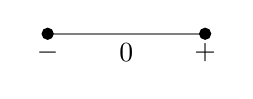
\begin{tikzpicture}
    \draw[gray, thick] (0,0) -- (2,0);
    \filldraw[black] (0,0) circle (2pt) node[anchor=north]{$-$};
    \filldraw[black] (2,0) circle (2pt) node[anchor=north]{$+$};
    \filldraw[black] (1,0) circle (0pt) node[anchor=north]{$0$};
    \end{tikzpicture}
\caption{$e_i$}
\end{figure}

This gives the desired association of each face with a sign vector. More concretely, for a face $f$, consider the possible values of a point $p = (p_1, p_2, \ldots, p_d)$ in $f$. Write its sign vector as $s = (s_1, s_2, \ldots, s_d)$. Now, if $p_i = 0$, then $s_i$ is $-$. If $p_i = 1$, then $s_i$ is $+$. If $0 \leq p_i \leq 1$, then $s_i = 0$. 

\smallskip

Given a linear function $f \in (\mathbb{R}^d)^*, f = (f_1, f_2, \ldots, f_d)$, we want to find the maximum point $p \in P$ to maximize $\langle f^T, p\rangle$. Consider the scaled cube $C_{d, f} = \boxplus_{i=1}^d [0,f_ie_i]$. We can easily find the maximum $c$ in $C_{d, f}$, which must be a vertex, by analyzing the sign of the vector $f^T$. The maximum $p \in P$ is then the closest point to $c$.

\smallskip
Let the generating points be $x_1, x_2, \ldots, x_n$, where $P = \conv(x_1, \ldots, x_n)$. We can tell if $y \in P$ by checking if there exists an convex combination

\[y = \sum_{i=1}^n \lambda_ix_i, \quad \sum_{i=1}^n \lambda_i \leq 1, \quad \lambda_i \geq 0\]

Then, if $y \not \in P$, consider a point $p\in P$ and connect edge $(p, y)$. Consider the affine plane of the face of $P$ which this edge intersects. This affine plane splits $P$ and y. Also, Farkas lemma IV later shows that if $y \notin P$, there exists a row vector $\bi{a}$ which separates $y$ from $P$, as in $\bi{ax} \leq \alpha$ is satisfied by all $\bi{x} \in P$, but not $\bi{y}$.
\end{solution}

\item Describe $C_d(d+2)$, the cyclic $d$-polytopes with $d+2$ vertices, combinatorially and explicitly.

\smallskip
Is the $2$-neighbor polytope $(\Delta_2 \times \Delta_2)^{\Delta}$ constructed in Example 0.5 combinatorially equivalent to $C_4(6)$?

\begin{solution}
The cyclic $d$-polytope on $n$ vertices is defined as 
\[C_d(n) = C_d(t_1, \ldots, t_n) = \conv(\textbf{x}(t_1), \ldots, \textbf{x}(t_n)) = \conv(\begin{pmatrix}
    t_1 \\
    t_1^2 \\
    \vdots \\
    t_1^d
\end{pmatrix}, \ldots, \begin{pmatrix}
    t_n \\
    t_n^2 \\
    \vdots \\
    t_n^d
\end{pmatrix}) \subseteq \mathbb{R}^d\]
where $n>d$ and $t_1 < t_2 < \ldots < t_n$.

Assume $d>1$. First notice that no $k$ of points $\textbf{x}(t_i)$ are contained in the same $k-2$ hyperplane. Also, the matrix

\[A = (\textbf{x}(t_1), \ldots, \textbf{x}(t_n))\]

has rank $d$ by the Vandermonde matrix identity (and $t_i \neq t_j$). Therefore $C_d(d+2)$ is of dimension $d$. 
    
For $d=2$ we have a quadrilateral $C_2(4)$ which is both simple and simplicial. $C_3(5)$ is the triangle bipyramid, which is simplicial and not simple. For $d>3$ we have that $C_d(d+2)$ is $2$-neighborly (this is stated as Corollary 0.8 in Ziegler without proof; it will be proved in exercise 0.8), meaning $\deg(v) = d+1$, thus $C_d(d+2)$ is simplicial and not simple. 

\smallskip
The $2$-neighbor polytope $(\Delta_2 \times \Delta_2)^{\Delta}$ is the polar of the product of two triangles. Ziegler describes:
\begin{quote}
"This is a $4$-polytope with $9$ vertices. It has $6$ facets, of the form ``edge of one triangle $\times$ the other triangle'': thus they all are triangular prisms. Furthermore, the intersection of two of them is either ``one of the triangles $\times$ a vertex of the other triangle,'' or it is ``an edge $\times$ an edge.'' In either case the intersection is $2$-dimensional. Hence any two facets of $P$ are adjacent, and $P^{\Delta} = (\Delta_{2} \times \Delta_{2})^{\Delta}$ is a $4$-polytope with $6$ vertices such that any two of them are adjacent."
\end{quote}

Both $(\Delta_2 \times \Delta_2)^{\Delta}$ and $C_4(6)$ are  $2$-neighborly $4$-polytopes 

A few observations. By Gale's evenness condition, $C_4(6)$ has exactly $9$ facets (dimension $3$, determined by $4$ vertices). $\Delta_2$ has $3$ vertices and the vertices of a product are exactly the products of the vertices. Therefore $\Delta_2 \times \Delta_2$ has $9$ vertices, which matches up in polarity. Furthermore, $\Delta_2 \times \Delta_2$ is simple and $C_4(6)$ is simplicial. 

To show they are combinatorially equivalent, it suffices to construct a bijection from the facets of $C_4(6)$ to the vertices of $\Delta_2 \times \Delta_2$. Set $t_i = i$ and the vertices of $\Delta_2$ to be $(0,0), (1,0), (0,1)$. The bijection is induced by the lexicographic order on both components.

\ermactually{that's cap bro}

\end{solution}

\item Consider the cyclic polytope $C_d(n) = \conv\{\textbf{x}(0), \textbf{x}(1), \ldots, \textbf{x}(n-1)\}$.
Show that there is an affine symmetry (an affine reflection) which induces the symmetry
$i \longleftrightarrow n-i-1$ (that is, $\textbf{x}(i-1) \longleftrightarrow \textbf{x}(n-i)$), and thus the
corresponding combinatorial symmetry of $C_d(n)$.
uy
\begin{remark}
    There are two mistakes in the original question statement, which have been corrected here.
\end{remark}
\begin{solution}
Write the affine transformation as $Ax+b$. Note that $b = \textbf{x}(n-1)$. Write $A_{d,n} = (a_{ij})_{d \times d}$ as the matrix for $C_d(n)$.

We claim that

\[A_{d, n} = \begin{pmatrix}
    -1 & 0 & 0 & \ldots & 0 \\
    -2(n-1) & 1 & 0 & \ldots & 0\\
    -3(n-1)^2 & 3(n-1) & -1 &  \ldots & 0 \\
    \vdots & \vdots & \vdots  & \ddots & \vdots \\
    -d(n-1)^{d-1} & d(n-1)^{d-2} & d(n-1)^{d-3} & \ldots & (-1)^{d}
\end{pmatrix}\]

A direct computation shows
\begin{align}
    A_{d,n}\textbf{x}(k) + b = 
    \begin{pmatrix}
        -k \\
        -2k(n-1) + k^2 \\
        -3k(n-1)^2 + 3k^2(n-1) - k^3 \\
        \vdots \\
        -dk(n-1)^{d-1} + \ldots +(-k)^d \\
    \end{pmatrix} + 
    \begin{pmatrix}
        n-1 \\
        (n-1)^2 \\
        (n-1)^3 \\
        \vdots \\
        (n-1)^d \\
    \end{pmatrix} = \textbf{x}(n-k-1)
\end{align}

Thus we are done.

The affine transformation induces a pairing of faces, with the only (non-trivial) exception as the vertex $\textbf{x}(\frac{n}{2})$ when $n$ is even.

\begin{comment}
The proof is by induction. First we show this for $C_2(n)$. Recall $b = \textbf{x}(n-1) = \begin{pmatrix}
    n-1 \\
    (n-1)^2
\end{pmatrix}$. We need to satisfy the following equations
\[\begin{cases}
    A\textbf{x}(1) + b = \textbf{x}(n-2) \\
    A\textbf{x}(2) + b = \textbf{x}(n-3) \\
    \vdots \\
    A\textbf{x}(n-2) + b = \textbf{x}(1)
\end{cases}\]

Directly checking, we have 

\begin{align*}
\begin{pmatrix}
    -1 & 0 \\
    -2(n-1) & 1 \\
\end{pmatrix}\textbf{x}(k) + b = 
\begin{pmatrix}
    n-k-1\\
    k^2 - 2k(n-1) +(n-1)^2 \\
\end{pmatrix} 
=\textbf{x}(n-k-1)
\end{align*}

Now we induct on $d$ for $C_d(n)$. Notice that induction fixes the upper left $d-1 \times d$ sub-matrix for $A_{d, n}$ as the block matrix $(A_{d-1, n}, \textbf{0})$. We want

\[A\textbf{x}(i) = \textbf{x}(n-i-1) - \textbf{x}(n-1)\]

for all $i$. 
This implies, for a row $i$ in $A$:

\[\sum_{j=1}^d k^ja_{ij} = (n-k-1)^i - (n-1)^i\]

NOTE: I am stupid.
\end{comment}
\end{solution}
\item From Gale's evenness condition, given in Theorem~0.7, derive a complete combinatorial description of all the faces of $C_d(n)$. From this, derive that the cyclic polytopes are $\bigl\lfloor \tfrac{d}{2} \bigr\rfloor$-neighborly (Corollary~0.8).

\begin{proof} The following is Gale's evenness condition. Note that it is an "if and only if" statement.
\begin{theorem*}
Let $n > d \ge 2$. We will use $[n]$ to denote the set $\{1,\dots,n\}$,
and choose real parameters $t_1 < t_2 < \cdots < t_n$.

The cyclic polytope
\[
  C_d(n) = \operatorname{conv}\{x(t_1),\dots,x(t_n)\}
\]
is a simplicial $d$-polytope. A $d$-subset $S \subseteq [n]$ forms a facet of $C_d(n)$ if and only if the following “evenness condition’’ is satisfied:

If $i < j$ are not in $S$, then the number of $k \in S$ between $i$ and $j$
is even:
\[
  2 \mid \#\{k : k \in S,\ i < k < j\}
  \quad\text{for } i,j \notin S.
\]
\end{theorem*}

From this condition, we can observe that for every set $S \subseteq [n]$, $|S| \leq \lfloor \frac{d}{2} \rfloor$, we can pick another set of at most $\lfloor \frac{d}{2} \rfloor$ numbers such that the numbers in $S$ are paired up with adjacent numbers. The rest can be put at an end of $[n]$. Since $C_d(n)$ is simplicial, any facet must be the $d-1$ simplex, and thus since $S$ is a subset of the vertex set of this simplex, it must be a face. It follows that the cyclic polytopes are $\lfloor \frac{d}{2} \rfloor$-neighborly.
\end{proof}
\item Show (bijectively) that the number of ways in which $2k$ elements can be chosen from $[n]$ in “even blocks of adjacent elements’’ is $\binom{n-k}{k}$. Thus, derive from Gale’s evenness condition that the formula for the number of facets of $C_d(n)$ is
\[
f_{d-1}(C_d(n))=\binom{\,n-\left\lceil\frac d2\right\rceil\,}{\left\lfloor\frac d2\right\rfloor}+\binom{\,n-1-\left\lceil\frac{d-1}2\right\rceil\,}{\left\lfloor\frac{d-1}2\right\rfloor},
\]
where $\lceil\cdot\rceil$ is the round-up function, with $\left\lceil\frac{k}{2}\right\rceil=k-\left\lfloor\frac{k}{2}\right\rfloor$. Here the first term corresponds to the facets for which the first block is even, and the second term corresponds to the cases where the first block is odd. Deduce
\[
f_{d-1}(C_d(n))=
\begin{cases}
\dfrac{n}{n-k}\binom{n-k}{k} & \text{for } d=2k \text{ even},\\[4pt]
2\binom{n-k-1}{k} & \text{for } d=2k+1 \text{ odd}.
\end{cases}
\]
How many facets do the cyclic polytopes $C_{10}(20)$, $C_{10}(100)$, and $C_{50}(100)$ have, approximately?

\begin{proof}
Co-identify each adjacent pair in each choice of $k$ adjacent pairs in $[n]$ and we obtain the desired bijection to choosing $k$ elements from $n-k$ elements, which is simply $\binom{n-k}{k}$. Then, a facet in $C_d(n)$ corresponds to choosing $d$ elements that either form adjacent pairs or are at the edge in $[n]$. If the first (leftmost) block is even, then if $d$ is even we simply obtain $\binom{n-\frac{d}{2}}{\frac{d}{2}}$. When $d$ is odd, we obtain $\binom{n-\frac{d+1}{2}}{\frac{d-1}{2}}$ because by Gale's evenness condition we must have the rightmost block as odd, which we can interpret as $n \in S$ and then choosing adjacent pairs from $[n-1]$. These both coincide with $\binom{n-\left\lceil\frac d2\right\rceil\,}{\left\lfloor\frac d2\right\rfloor}$, which is the first term. Now, if the first block is odd, we can interpret it as $1 \in S$ and choosing the rest from $[n] \setminus \{1\}$. The second term follows by similar reasoning as before, 

\begin{remark}
    We acknowledge this isn't the prettiest explanation. Umm, it works though.
\end{remark}

So now, if $d = 2k$, we get 

\[f_{d-1}(C_d(n)) = \binom{n-k}{k} + \binom{n-1-k}{k-1} = \left( 1 - \frac{k}{n-k}\right)\binom{n-k}{k} = \frac{n}{n-k}\binom{n-k}{k}.\]

And, if $d=2k+1$, we get

\[f_{d-1}(C_d(n)) = \binom{n-(k+1)}{n-k} + \binom{n-1-k}{k} = 2\binom{n-k-1}{k}.\]

With this we can easily compute the number of facets for the cyclic polytopes: $f_9(C_{10}(20)) = 4004$, $f_9(C_{10}(100)) = 60990020$, and $f_{49}(C_{50}(100)) = 70118062854865191504$.
\end{proof}

\item Show that if a polytope is $k$-neighborly, then every $(2k-1)$-face is a simplex. Conclude that if a $d$-polytope is $(\lfloor \frac{d}{2} \rfloor + 1)$-neighborly, then it is a simplex.

\begin{proof}
    Let $P$ be a $k$-neighborly polytope and label the vertices of a $(2k-1)$-face $F$ as $[n]$. We can assume $P = F$. It suffices to show that $n = 2k$. Assume by contradiction $n > 2k$. Because $P$ is $k$-neighborly, any $k$ vertices must be linearly independent

    \ermactually{bro idk bro wtf is this bro}
\end{proof}

\item* Is there a fast and simple way to decide whether a certain point $x\in\mathbb{R}^d$ (with rational coordinates, say) is contained in the cyclic polytope $C_d(1,2,\ldots,n)$? 

(General theory — namely the polynomial equivalence of optimization and separation according to Gr\"otschel, Lov\'asz \& Schrijver [246] — implies that there is a polynomial algorithm for this task, since optimization over $C_d(n)$ is easy, by comparing the vertices. However, we ask for a simple combinatorial test, not using the ellipsoid method.)

\item Prove the claims in Example~0.12 about the Birkhoff polytope $P(d)$: in particular, show that the dimension is $(d-1)^2$, and that the number of facets is $d^2$. The Birkhoff polytope $P(d)$ and the permutahedron $\Pi_{d-1}$ are closely related: show that there is a canonical projection map $P(d)\to \Pi_{d-1}$.

\begin{proof}
    The first two parts follow from the solution to Exercise 1.9, as Birkhoff polytopes are a special case of transportation polytopes. Let the columns of $X \in P(D)$ be $\bi{x}_1, \ldots, \bi{x}_{d}$. The projection map is $\pi: P(d) \to \Pi_{d-1},\; \pi(X) = \sum_{k=1}^d k\bi{x}_k$. Note that $k$ can actually be substituted with $\sigma(k)$ for any $\sigma \in S_d$.
\end{proof}

\item Draw the 3-dimensional associahedron $K_{3}$. Justify the general
formula $\frac{1}{n} \binom{2n-2}{n-1}$ for the number of vertices of $K_{n-2}$.

\begin{solution}
 
Behold, The 3-dimensional associahedron $K_3$.

\begin{figure}[H]
    \centering

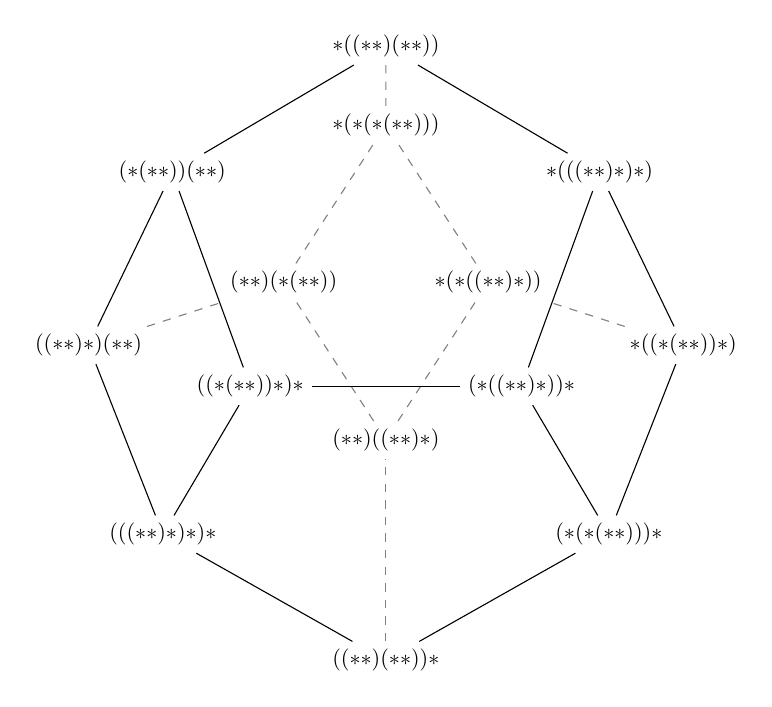
\begin{tikzpicture}[x=1.18mm,y=1mm,scale=2,>=stealth]
  \tikzset{every node/.style={scale=.8}}
  
  \node (1120) at (-7.3,-1.6)  {$((\ast(\ast\ast))\ast)\ast$};
  \node (1210) at ( 7.3,-1.6)  {$(\ast((\ast\ast)\ast))\ast$};
  \node (3010) at ( 0, 20)     {$\ast((\ast\ast)(\ast\ast))$};
  \node (1201) at ( 0,-19)     {$((\ast\ast)(\ast\ast))\ast$};
  \node (2011) at (-16, 1)     {$((\ast\ast)\ast)(\ast\ast)$};
  \node (2200) at ( 16, 1)     {$\ast((\ast(\ast\ast))\ast)$};
  \node (2020) at (-11.5,12)   {$(\ast(\ast\ast))(\ast\ast)$};
  \node (2110) at ( 11.5,12)   {$\ast(((\ast\ast)\ast)\ast)$};
  \node (1111) at (-12,-11)    {$(((\ast\ast)\ast)\ast)\ast$};
  \node (1300) at ( 12,-11)    {$(\ast(\ast(\ast\ast)))\ast$};
  \node (4000) at ( 0, 15)     {$\ast(\ast(\ast(\ast\ast)))$};
  \node (2101) at ( 0, -5)     {$(\ast\ast)((\ast\ast)\ast)$};
  \node (3001) at (-5.5, 5)    {$(\ast\ast)(\ast(\ast\ast))$};
  \node (3100) at ( 5.5, 5)    {$\ast(\ast((\ast\ast)\ast))$};

  \path[-,dashed,color=black!50!white]
    (2011) edge (3001)
    (2200) edge (3100)
    (1201) edge (2101)
    (3010) edge (4000)
    (2101) edge (3001)
    (3001) edge (4000)
    (2101) edge (3100)
    (3100) edge (4000);

  \path[-]
    (1120) edge (1210)
    (1210) edge (2110)
    (2110) edge (3010)
    (1120) edge (2020)
    (2020) edge (3010)
    (1210) edge (1300)
    (1111) edge (1120)
    (1111) edge (1201)
    (1201) edge (1300)
    (1111) edge (2011)
    (2011) edge (2020)
    (1300) edge (2200)
    (2110) edge (2200);
\end{tikzpicture}

\caption{The Associahedron $K_3$}
\end{figure}

Now we show by strong induction that $K_{n-2}$ has $\frac{1}{n}\binom{2n-2}{n-1}$ vertices. One can easily check that $|V(K_1)| = \frac{1}{n}\binom{2n-2}{n-1} = 2$ for $n=3$. Notice that we can partition $n+1$ according to the following
\[\begin{cases}
    (n-1)(1) \\
    (n-2)(2) \\
    \vdots \\
    (\lceil \frac{n}{2}\rceil)(\lfloor \frac{n}{2} \rfloor)\\
    \vdots \\
    (2)(n-2) \\
    (1)(n-1)\\
\end{cases}\]
Thus we get the recurring formula:
\[   ||V(K_n)| = \sum_{k=1}^{n-1} |V(K_k)||(V(K_{n-k})| \]

The algebraic proof is tedious and difficult. Write $|V(K_n)| = C_n$ and consider the generating function $f(x) = \sum_{i=0}^{\infty} C_ix^i$, where $C_0 = 1$. Then it suffices to show that $f(x)= xf(x)^2+1$.

Now we claim that $f(x) = \frac{1-\sqrt{1-4x}}{2x}$. By the generalized binomial theorem,

\[(1-4x)^{1/2} = \sum_{k=0}^{\infty} \binom{1/2}{k}(-4x)^k\]

Thus, we have 

\[\frac{1-\sqrt{1-4x}}{2x} = \frac{1-\sum_{k=0}^{\infty} \binom{1/2}{k}(-4x)^k}{2x} = \sum_{k=1}^{\infty} \frac{-\binom{1/2}{k}(-4x)^k}{2x} = \sum_{k=0}^{\infty} a_kx^k\]

Where we have $a_k = 2\binom{1/2}{k+1}(-4)^{k}$.

Expanding $\binom{1/2}{k+1}$, we have
\[\binom{1/2}{k+1} = \frac{\frac{1}{2}(\frac{1}{2}-1)\ldots(\frac{1}{2}-k)}{(k+1)!} = (-1)^k \frac{(2k+1)!!}{2^{k+1}(k+1)!} = (-1)^k \frac{(2k+1)!}{2^{2k+1}(k!)(k+1)!}\]

Thus, we have
\[a_k = 2(-1)^k \frac{(2k+1)!}{2^{2k+1}(k!)(k+1)!}(-4)^{k} = \frac{1}{k+1}\binom{2k}{k}\]
as desired.

We can now directly compute $f(x)^2$

\[f(x)^2 = \left(\frac{1-\sqrt{1-4x}}{2x} \right)^2 = \frac{2-4x-2\sqrt{1-4x}}{4x^2}\]

Therefore, we have

\[xf(x)^2 + 1 = \frac{2-4x-2\sqrt{1-4x}}{4x} + 1 = \frac{1-\sqrt{1-4x}}{2x} = f(x)\]

which proves the formula $||V(K_n)| = \sum_{k=1}^{n-1} |V(K_k)||(V(K_{n-k})|$, as desired.
\end{solution}

\item Describe the combinatorial structure of the traveling salesman polytopes $Q_T(3)$, $Q_T(4)$, and $Q_T(5)$. How many vertices and facets do they have? Which vertices are adjacent? Are they simple, or simplicial? Similarly, try to describe $Q'_T(2)$, $Q'_T(3)$, and $Q'_T(4)$.

\begin{solution}
    Label the set of vertices in $K_n$ as $[n]$. The traveling salesman polytope $Q_T(n)$ consists of all the tours of $K_n$, which we can essentially think of as elements in the quotient group $S_n/(C_n\times C_2)$, which gives the vertex count $\frac{n!}{2n} = \frac{(n-1)!}{2}$, the number of Hamiltonian tours through $K_n$. 
    \ermactually{im ngl idk how to think about these monsters}
\end{solution}


\item * What is the maximal number $f(d)$ of facets of a $d$-dimensional $0/1$-polytope? How fast does $f(d)$ grow asymptotically?
(It is not hard to see that
\[2^{d} \le f(d) \le d! + 2d .\]

The upper bound was suggested by Imre Bárány, via the following observation: if we add the “missing vertices’’ of the $d$-cube to the polytope one by one, then we add a volume of at least $1/d!$ for every facet that is destroyed of the original $0/1$-polytope. The process will stop with the $d$-cube of volume $1$, with only $2d$ facets.

More recent progress on this problem is recorded in work of Kortenkamp, Richter-Gebert, Sarangarajan and Ziegler [343]. Still, there is a huge gap between the lower and the upper bounds. We know
\[f(1)=2,\quad f(2)=4,\quad f(3)=8,\quad f(4)=16,\]
\[f(5)=40,\quad 121 \le f(6) \le 610,\quad \textit{etc.}\]
for small dimensions. (See Aichholzer [5,6] for enumeration techniques.) Asymptotically the best known bounds are
\[(3.6)^{d} < f(d) \le 30\,(d-2)!\]

for all large enough $d$. Here the upper bound is due to Fleiner, Kaibel and Rote [206], while the lower bound is from explicit computation of “random $0/1$-polytopes’’ in low dimensions in combination with a “free sum’’ construction for $0/1$-polytopes from [343]. The value $3.6$ was achieved in March 1997 by Thomas Christof for a random $0/1$-polytope (of dimension $13$, with $254$ vertices and \textit{at least} $17{,}464{,}356$ facets), using his PORTA code and new ideas described in work with Reinelt [155]. 

For “current records’’ in the “Olympic race’’ for $0/1$-polytopes with many facets see [342] on the Web.)

\item Via the construction of “characteristic vectors’’ from Example~0.13, show that the vertices of the Birkhoff polytope $P(n)$ correspond to the perfect matchings in the complete bipartite graph $K_{n,n}$.

\begin{solution}
    Each vertex in the Birkhoff polytope $P(n)$ corresponds to a representation of a element in $S_n$ in $\mathbb{R}^{n \times n}$. Each column $\bi{x}_i$ of a vertex has exactly one entry $x_{ij} = 1$ and the rest are $0$. Thus we can interpret $X \in P(n)$ as that each $x_{ij} = 1$ means that we should match $i$ from the left to $j$ from the right. Equivalently, think of the identity perfect matching and consider each $\sigma \in S_n$ (corresponding to the element $X^\sigma \in P(n)$) acting on (permuting) the right-hand vertices in $K_{n,n}$. 
\end{solution}

\item Show that the Birkhoff polytope $P(d) \subseteq \mathbb{R}^{d^{2}}$ contains the asymmetric traveling salesman polytope $Q'_{T}(d) \subseteq \mathbb{R}^{d^{2}-d} \subseteq \mathbb{R}^{d^{2}}$. Does every facet of $P(d)$ yield a facet of $Q'_{T}(d)$?
(For a detailed investigation, see Billera and Sarangarajan [76].)

\begin{remark}
    We believe Ziegler meant 'asymmetric' and simply mistyped $Q'_T(d)$ as $Q_T(d)$ in the original question statement. It has been corrected here, and we will proceed to answer as such.
\end{remark}

\begin{solution}
    Fix a vertex labeling $[d]$ on $\vec K_d$ (the directed complete graph). For each element in $Q'_T(d)$ we can write it as a permutation on the vertex set $[d]$ according to its path (the starting point technically doesn't matter, but fixing something also works). The containment becomes clear because $P(d)$ consists of all the elements of $S_d$.

    \ermactually{what about the facets hmm?}
\end{solution}
\end{enumerate}
\bigskip
\section{Polytopes, Polyhedra, and Cones}

\begin{enumerate}
\setcounter{enumi}{-1}
\renewcommand{\labelenumi}{1.\arabic{enumi}}
\item If we try to restrict the proof of Theorem 1.2 to polytopes, where does this fail? In other words, where do we use a construction that necessarily takes us from polytopes to unbounded polyhedra?
\begin{solution}
    $\elim_k(P)$ is always unbounded in the direction $e_k$, which means that $\proj_k(P) = \elim_k(P) \cap \{x \in \mathbb{R}^k: x_k = 0\}$ is not guaranteed to be a polytope again.

\begin{remark}
    The proof can be rectified
\end{remark}
\end{solution}

\item Do experiments with the methods of this chapter on some examples:
\begin{enumerate}[label=(\roman*)]
\item Compute the vertices of the 2-dimensional example of Section 1.2. Check carefully that everything you get actually is a vertex.
  
\item Compute defining inequalities for the cyclic polytope $C_3(6)$, for example for $t_i = i$. For every inequality, find the set of vertices that satisfy it with equality.
  
\item Find the facets of the 4-polytopes of the Exercises 4.8.6 and 4.8.15 from Grünbaum [252, pp. 64, 65].
  
\item These were Mickey-Mouse examples (i.e., very small). For more realistic ones, find all the facets of the traveling salesman polytopes $Q_T(6)$, $Q_T(7)$, $Q_T(8)$, and of the asymmetric travelling salesman polytopes $Q'_T(5)$ and $Q'_T(6)$. (Better use a computer; $Q_T(8)$ is a 20-dimensional polytope with 2520 vertices and $194,187$ facets~[153]. The polytope $Q_T(9)$ has $42,104,442$ facets; for $Q_T(10)$ Christof found $51,043,900,866$ facets and conjectures that they give a complete description --- see [152] and [154]. Similarly, Euler \& Le Verge~[200] have derived a description of $Q'_T(6)$: a 19-dimensional polytope with 120 vertices and $319,015$ facets.)
\end{enumerate}

\begin{solution} The calculations are omitted. Here are the results.
\begin{enumerate}[label=(\roman*)]
    \item The vertices are $\{(-1, -2), (-3, -\frac{3}{2}), (4, 2), (4, 3), (\frac{7}{2}, 4), (\frac{1}{2}, 3)\}$. The redundant vertices (intersections of lines of equality for the inequalities) can be determined by comparing points. If there exists $v, v'$ such that (WLOG) $v \leq v'$ component wise, then $v'$ redundant. The direction of the inequality is determined by the direction of the inequalities for the intersecting inequalities (consider the sides which they contain).

    \item Recall that all cyclic polytopes are simplicial. The facets for $C_3(6) = C_3(\textbf{x}(0), \textbf{x}(1), \ldots, \textbf{x}(5))$ are (by Gale's evenness)
    \[\{\{1,2,3\}, \{1,3,4\}, \{1,4,5\}, \{1,5,6\}, \{1,2,6\}, \{2,3,6\}, \{3,4,6\}, \{4,5,6\}\}\]
    The inequalities can be found through a simple calculation.

    \item skipped 

    \item skipped
\end{enumerate}
\end{solution}

\item Describe a Fourier-Motzkin elimination method to solve strict inequality systems $\{x : Ax < z\}$. Use it to prove a representation theorem for ``open polyhedra.''

\begin{solution}
    Nothing has to be changed except for a strict inequality ($<$ instead of $\leq$) between the lower and upper bounds. The rest is the same
\end{solution}

\item Show that if $C = \cone(W)$ for any cone in $\mathbb{R}^{d+1}$ generated by arbitrary vectors $\bi{x}_i$ (not necessarily with $w_{i0} \geq 0$, then $\{\bi{x} \in \mathbb{R}^d : \begin{pmatrix}
    1 \\
    {\bi{x}}
\end{pmatrix} \in C\}$ is a $\mathcal{V}$-polyhedron.

\begin{proof}
    $\{\bi{x} \in \mathbb{R}^d : \begin{pmatrix}
    1 \\
    {\bi{x}}
\end{pmatrix} \in C\}$ is a slice of the cone. Namely, it is $C \cap \{\bi{x}\in \mathbb{R}^d: \bi{x}_0 = 1\}$. Theorem 1.2 (Main Theorem for Polyhedra) says that the cone is also $\mathcal{H}$-polyhedron, Fourier-Motzkin says that the slice of a $\mathcal{H}$-polyhedra is again a $\mathcal{H}$-polyhedra, and another use of Theorem 1.2 concludes the proof.
\end{proof}

\item State and prove a Farkas lemma for systems of the form
$A\bi{x} \le \bi{z},\; \bi{x} \ge \textbf{0}.$

\begin{solution}
We propose the following lemma
\begin{lemma*}[FL for nonnegative $\bi{x}$]
    Let $A \in \mathbb{R}^{m \times d}$, and $\bi{x} \in \mathbb{R}^m$.

    \textbf{Either} there exists a point $\bi{x} \in \mathbb{R}^d, \bi{x} \geq \textup{\textbf{0}}$, such that $A\bi{x} \leq \bi{z}$,
    
    \textbf{or} there exists a row vector $\bi{c} \in (\mathbb{R}^m)^*$  with $\bi{c}A \geq \mathds{O}$ and $\bi{cz} < 0$, 
    
    but not both. 
    
\end{lemma*}

\begin{proof}
We have the following equivalences:
\begin{flalign*}
    & \exists \bi{x}: A\bi{x} \leq \bi{z}, \; \bi{x} \geq 0 &\\
    & \iff \exists \bi{x} : \begin{pmatrix}
        A \\ -I_d
    \end{pmatrix} \bi{x} \leq \begin{pmatrix}
        \bi{z} \\ \textbf{0}
    \end{pmatrix} \\
    & \overset{\text{FL I}}{\iff}  \nexists \bi{c}, \bi{b} \geq \mathds{O}, \; (\bi{c}, \bi{b}) \begin{pmatrix}
        A \\ -I_d
    \end{pmatrix} = \mathds{O}, \; (\bi{c}, \bi{b}) \begin{pmatrix}
        \bi{z} \\ \textbf{0}
    \end{pmatrix} < 0\\
    & \iff \nexists \bi{c}, \bi{b} \geq \mathds{O}, \; \bi{c}A = \bi{b}, \; \bi{cz} < 0  \\
    & \iff \nexists \bi{c} \geq \mathds{O}, \; \bi{c}A \geq \mathds{O}, \; \bi{cz} < 0.
\end{flalign*}
\end{proof}
\end{solution}

\item Prove the following Farkas lemma for equality and inequality constraints:
for compatible matrices $A,B,C$ and vectors $\bi{u}, \bi{v}, \bi{w}$
either there exists a solution vector $\bi{x}$ for
\[
A\bi{x} = \bi{u},\quad
B\bi{x} \ge \bi{v},\quad
C\bi{x} \le \bi{w},
\]
or there exist row vectors $\bi{a}, \bi{b}, \bi{c}$ with
\[
\bi{a}A + \bi{b}B + \bi{c}C = 0,\quad
\bi{b} \le \mathds{O},\quad
\bi{c} \ge \mathds{O},\quad
\bi{a}\bi{u} + \bi{b}\bi{v} + \bi{c}\bi{w} < 0.
\]

\begin{proof}
We have the following equivalences
\begin{flalign*}
    & \exists \bi{x}: A\bi{x} = \bi{u}, \; B\bi{x} \geq \bi{v}, \; C\bi{x} \leq \bi{w} &\\
    &\iff \exists \bi{x}: A\bi{x} \leq \bi{u}, \; A(-\bi{x}) \leq -\bi{u}, \; B(-\bi{x}) \leq -\bi{v}, \; C\bi{x} \leq \bi{w} \\
    & \iff \exists \bi{x}: \begin{pmatrix}
        A \\ -A \\ -B \\ C
    \end{pmatrix}\bi{x} \leq \begin{pmatrix}
        \bi{u} \\ -\bi{u} \\ -\bi{v} \\ \bi{w}
    \end{pmatrix} \\
    & \overset{\text{FL I}}{\iff} \nexists \bi{a}_1, \bi{a}_2, \bi{b}_1, \bi{c} \geq \mathds{O}, \; (\bi{a}_1, \bi{a}_2, \bi{b}_1, \bi{c})\begin{pmatrix}
        A \\ -A \\ -B \\ C
    \end{pmatrix} = \mathds{O}, \; (\bi{a}_1, \bi{a}_2, \bi{b}_1, \bi{c})\begin{pmatrix}
        \bi{u} \\ -\bi{u} \\ -\bi{v} \\ \bi{w}
    \end{pmatrix} < 0 \\
    & \iff \nexists \bi{a}_1, \bi{a}_2, \bi{b}_1, \bi{c} \geq \mathds{O}, \; (\bi{a}_1 - \bi{a}_2)A - \bi{b}_1B + \bi{c}C = \mathds{O}, \; (\bi{a}_1 - \bi{a}_2)\bi{u} - \bi{b}_1\bi{v} + \bi{c}\bi{w} < 0.
\end{flalign*}

Writing $\bi{a} = (\bi{a}_1 - \bi{a}_2)$ and $\bi{b} = -\bi{b}_1$ gives the desired result.
\end{proof}

\item Prove the following general Farkas lemma for equality and inequality constraints: for compatible matrices $A, B, C, D$ and vectors $\bi{z},\bi{w}$ either there exist solution vectors $\bi{x},\bi{y}$ for
\[
A\bi{x} + B\bi{y} \le \bi{z},\quad
C\bi{x} + D\bi{y} = \bi{w},\quad
\bi{x} \ge \textbf{0},
\]
or there exist row vectors $\bi{c},\bi{d}$ with
\[
\bi{c}A + \bi{d}C \ge \mathds{O},\quad
\bi{c}B + \bi{d}D = \mathds{O},\quad
\bi{c} \ge \mathds{O},\quad
\bi{c}\bi{z} + \bi{d}\bi{w} < 0.
\]

\begin{proof}
Define $\bi{s} := \bi{z} - (A\bi{x} + B\bi{y})$. Note $\bi{s} \geq \textbf{0}$. Now decompose $\bi{y} = \bi{y}^+ - \bi{y}^-$, such that $\bi{y}^+, \bi{y}^- \geq \textbf{0}$. 

We have the following equivalences
\begin{flalign*}
    & \exists \bi{x}, \bi{y}^+, \bi{y}^-, \bi{s} \geq \textbf{0}: \begin{pmatrix}
        A & B & -B & I \\ C & D & -D & \textbf{0}
    \end{pmatrix} 
    \begin{pmatrix}
        \bi{x} \\ \bi{y}^+ \\ \bi{y}^- \\ \bi{s}
    \end{pmatrix} = 
    \begin{pmatrix}
        \bi{z} \\ \bi{w} 
    \end{pmatrix} &\\
    & \overset{\textup{FL II}}{\iff} \nexists (\bi{c}, \bi{d}) \in (\mathbb{R}^?)^*: (\bi{c}, \bi{d})
    \begin{pmatrix}
        A & B & -B & I \\ C & D & -D & \textbf{0}
    \end{pmatrix} \geq \mathds{O}, \; (\bi{c}, \bi{d})
    \begin{pmatrix}
        \bi{z} \\ \bi{w} 
    \end{pmatrix} < 0 \\
    & \iff  \nexists \bi{c}, \bi{d}: \bi{c} \geq \mathds{O}, \; \bi{c}A + \bi{d}C \geq \mathds{O}, \; \bi{c}B + \bi{d}D = \mathds{O}, \; \bi{cz} + \bi{dw} < 0.
\end{flalign*}

Thus we are done.
\end{proof}

\item State and prove a version of Carathéodory’s theorem for convex–conical combinations.

\begin{solution}
We state the following
\begin{theorem*}[Carathéodory for $\mathcal{V}$-polytopes]
Let $V \in \mathbb{R}^{d \times n}$, $Y \in \mathbb{R}^{d \times n'}$, $\bi{x} \in \mathbb{R}^d$. If $\bi{x} \in \conv(V) \boxplus \cone(Y)$, then $\bi{x} \in \conv(V') \boxplus \cone(Y')$ holds for subsets $V' \subseteq V$, $Y' \subseteq Y$ of at most $\dim\conv(V)$, $\dim\cone(Y) + 1$ vectors in $V$, $Y$, respectively.
\end{theorem*}
\begin{proof}
We have the biconditional:
\[\bi{x} \in \conv(V) \boxplus \cone(Y) \iff \bi{v} \in \conv(V), \bi{y} \in \conv(Y), \bi{v} \boxplus \bi{y} = \bi{x}\]
Now notice:
\[\bi{x} \in \conv(V) \iff \begin{pmatrix}
    1 \\ \bi{x}
\end{pmatrix} \in \cone\begin{pmatrix}
    \mathds{1} \\ V
\end{pmatrix}\]
Thus, the theorem follows by standard Carathéodory.
\end{proof}
\end{solution}

\item Transportation polytopes have the form
\[
P(d : \bi{a}, \bi{b})
=\left\{
X\in\mathbb{R}^{d\times d} :
\begin{array}{l}
x_{ij}\ge 0 \ (1\le i,j\le d),\\[4pt]
\sum_{k=1}^d x_{ik}=a_i \ (1\le i\le d),\\[4pt]
\sum_{k=1}^d x_{kj}=b_j \ (1\le j\le d)
\end{array}
\right\}.
\]

Study transportation polytopes. Determine the dimension. Interpret vertices and facets. Show that the Birkhoff polytopes are special transportation polytopes. Show that non-empty transportation polytopes $P(d : \bi{a}, \bi{b})$ have canonical center points $x_{ij}=\frac{a_i b_j}{\Lambda},\; \Lambda := \sum_{k=1}^d a_k = \sum_{k=1}^d b_k.$

\begin{solution}
Transportation polytopes have dimension $(d-1)^2$ (assuming that no $a_i$ or $b_j$ is $0$). In general, for $X \in \mathbb{R}^{m\times n}$, the dimension is $(m-1)(n-1)$. This is exactly the number of 'free' variables in each row/column, because we have $\sum_{k=1}^m x_{ik}=a_i$, and a redundant variable, which comes from $\sum_{i=1}^m a_i = \sum_{j=1}^n b_j$. The general formula applies to a degenerate transportation polytope, where some column or row sums are $0$. One can see that $X \in \mathbb{R}^{(d - \textup{\# of zeroes in } \bi{a}) \times (d - \textup{\# of zeroes in } \bi{b})}$.

\ermactually{I am going to come back to this problem.}


\end{solution}

\item Interpret the Farkas lemma IV as a statement about polyhedra, and observe that it follows “trivially” from the equivalence of $\mathcal{V}$ - and $\mathcal{H}$-polyhedra (Theorem 1.2).  
Derive Farkas lemma II from Farkas lemma IV, and then Farkas lemma I from Farkas lemma II.  
(This alternative route through the jungle of Farkas lemmas was suggested by Joe Bonin.)

\smallskip
We restate FL IV for clarity:

\begin{lemma*}[FL IV]
Let $V\in\mathbb{R}^{d\times n}$, $Y\in\mathbb{R}^{d\times n'}$, and $\bi{x}\in\mathbb{R}^d$.

\textbf{Either} there exist $\bi{t},\bi{u}\ge \textbf{0}$ with $\mathds{1}\bi{t}=1$ and $\bi{x}=V\bi{t}+Y\bi{u}$,

\textbf{or} there exists a row vector $(\alpha, \bi{a}) \in (\mathbb{R}^{d+1})^*$ with 
$\bi{a}v_i \le \alpha$ for all $i \le n$, $\bi{a} y_j \le 0$ for all $j \le n'$,
while $\bi{a}\bi{x} > \alpha$,

but not both.
\end{lemma*}

\begin{solution}

Farkas lemma IV can be alternatively characterized as that, for a point $\bi{x}$ and a polyhedron $P$, \textbf{Either} $\bi{x} \in P$ (through the $\mathcal{V}$-polyhedron perspective), \textbf{or} $\bi{x}$ can be separated from $P$ by a linear functional (as in the $\mathcal{H}$-polytope perspective). Therefore it follows directly from lemma 1.2, the main theorem for polyhedra.

\smallskip
Starting here, we derive FL II then FL I.

\begin{proposition*}[FL II, from FL IV]
Let $A\in\mathbb{R}^{m\times d}$ and $z\in\mathbb{R}^m$.

\textbf{Either} there exists a point $\bi{x}\in\mathbb{R}^d$ with 
$A\bi{x}=\bi{z}$, $\bi{x}\ge \textbf{0}$,

\textbf{or} there exists a row vector $\bi{c}\in(\mathbb{R}^m)^*$ with 
$\bi{c}A\ge \mathds{O}$ and $\bi{cz}<0$,

but not both.
\end{proposition*}
\begin{proof}
Taking $V$ = \textbf{0} in FL IV, we have the following equivalences
\begin{flalign*}
    & \exists \bi{t},\bi{u}\ge \textbf{0}, \mathds{1} \bi{t}=1: \bi{x}=V\bi{t}+Y\bi{u} &\\
    & \iff \exists \bi{u} \ge \textbf{0}:  \bi{x} = Y\bi{u} \\
    & \overset{\textup{FL IV}}{\iff} \nexists (\alpha, \bi{a}) \in (\mathbb{R}^{d+1})^*: \bi{a}V \leq \alpha \mathds{1}, \; \bi{a}Y \leq \mathds{O}, \; \bi{ax} > \alpha \\
    & \iff \nexists (\alpha, \bi{a}) \in (\mathbb{R}^{d+1})^*: 0 \leq \alpha, \; (-\bi{a})Y \geq \mathds{O}, (-\bi{a})\bi{x} < -\alpha.
\end{flalign*}

From which, letting $\alpha = 0$ (we can do this because it is the 'best case scenario') and relabeling variables, we obtain the desired proposition.
\end{proof}

We now prove FL I
\begin{proposition*}[FL I, from FL II]
Let $A\in\mathbb{R}^{m\times d}$ and $\bi{z}\in\mathbb{R}^m$.

\textbf{Either} there exists a point $\bi{x}\in\mathbb{R}^d$ with 
$A\bi{x}\le \bi{z}$,

\textbf{or} there exists a row vector $\bi{c}\in(\mathbb{R}^m)^*$ with 
$\bi{c}\ge \mathds{O}$, $\bi{c}A=\mathds{O}$ and $\bi{cz}<0$,

but not both.
\end{proposition*}
\begin{proof}
Define $\bi{s} = \bi{z}-A\bi{x}$, and note that $\bi{s} \geq 0$. Now decompose $\bi{x} = \bi{x}^+ - \bi{x}^-$, where $\bi{x}^+, \bi{x}^- \geq 0$. Thus we have the following equivalences
\begin{flalign*}
    & \exists \bi{x}^+, \bi{x}^-, \bi{s} \geq \textbf{0}: (A, -A, I)\begin{pmatrix}
    \bi{x}^+ \\ \bi{x}^- \\ \bi{s}
\end{pmatrix} = \bi{z} & \\
    & \overset{\textup{FL II}}{\iff} \nexists \bi{c}: \bi{c}(A, -A, I) \geq \mathds{O}, \; \bi{cz} < 0 \\
    & \iff \nexists \bi{c}: \bi{c}A = \mathds{O}, \; \bi{c} \geq \mathds{O}, \; \bi{cz} < 0.
\end{flalign*}
Thus we are done.
\end{proof}
\end{solution}
\end{enumerate}

\bigskip
\section{Faces of Polytopes}
\begin{enumerate}
\setcounter{enumi}{-1}
\renewcommand{\labelenumi}{2.\arabic{enumi}}
\item Let $P$ be a polyhedron and let $F_0$ be any nonempty face of $P$ which is minimal with respect to inclusion. Taking $\bi{x}_0 \in F_0$, show that $F_0 - \bi{x}_0$ is a linear subspace, and that
\[F_0 -\bi{x}_0 = \operatorname{lineal}(P).\]
Thus, if $P$ has lineality space $\lineal(P) = \{\textbf{0}\}$, then every minimal nonempty face is a vertex — and in particular, $P$ has a vertex.
\begin{remark}
    $F_0 - \bi{x}_0$ here means shifting the affine subspace $F_0$ by the vector $\bi{x}_0$.
\end{remark}
\begin{proof}

The face (affine subspace) $F_0$ can be written as $P \cap \{\bi{x}: \bi{cx} = \alpha\}$ for some $\alpha$. Since $\bi{x}_0 \in F_0$, we have $\bi{cx}_0 = \alpha$, and so for every $\bi{x} \in F_0$ we get $\bi{c} (\bi{x} - \bi{x}_0)= 0$. Therefore, $F_0 - \bi{x}_0$ is translated to the origin. We can check

\[\lambda(\bi{x}-\bi{x}_0) + (1-\lambda)(\bi{y} - \bi{y}_0) = \lambda \bi{x} + (1-\lambda)\bi{y} - \bi{x}_0\]

and 

\[\bi{w} \in F_0 - \bi{x}_0 \iff \bi{w} + \bi{x}_0 \in F_0\]

So, to show that $F_0 - \bi{x}_0$ is linear, we show, for $\bi{u}, \bi{v} \in F_0$:

\[\lambda(\bi{u} - \bi{x}_0) = \lambda(\bi{u} - \bi{x}_0) + (1-\lambda)(\bi{x}_0 - \bi{x}_0) \in F_0 - \bi{x}_0\]

and then 

\[(\bi{u} - \bi{x}_0) + (\bi{v} - \bi{x}_0) = \frac{1}{2}\cdot 2(\bi{u} - \bi{x}_0) + \frac{1}{2}\cdot 2(\bi{v} - \bi{x}_0) \in F_0 - \bi{x}_0\]

which shows $F_0 - \bi{x}_0$ is linear.

\smallskip
Now, recall
\[\lineal(P):= \{\bi{y} \in \mathbb{R}^d: \bi{x}+t\bi{y} \in P \textup{ for all }\bi{x} \in P, t \in \mathbb{R}\}.\]

Indeed, we have $\bi{x}_0 \in (\lineal(P) + \bi{x}_0) \cap P$. Since $F_0$ was minimal, we get $F_0 \subseteq (\lineal(P) + \bi{x}_0) \cap P$, which gives $F_0 - \bi{x}_0 \subseteq \lineal(P)$. Now for the sake of contradiction assume $\exists \bi{y} \in \lineal(P)$ such that $\bi{y} \notin F_0 - \bi{x}_0$. By taking $\bi{x} = \bi{x}_0$, it follows that $t\bi{y}+\bi{x}_0 \in P$ and not in $F_0$, for all $t\in \mathbb{R}$. But then we get $\bi{c}(t\bi{y}+\bi{x}_0) < \alpha$ (the inequality is strict since $t\bi{y} + \bi{x}_0 \notin F_0$, which gives $\bi{c}t\bi{y} < 0$. Since this must hold for all $t \in \mathbb{R}$, we see that the not all of $P$ satisfies $\bi{cx} \leq \alpha$, meaning it is not a face, which is a contradiction. It follows that $\lineal(P) = F_0 - \bi{x}_0$

\end{proof}

\item Use the previous exercise combined with Theorem 1.2 to formulate and prove analogues of the Representation Theorem 2.15 for polyhedra. Special attention is needed for the formulation of part (5). In particular, what do you get in the case where $P$ is a cone?

\begin{solution}
Theorem 1.2 is the main theorem for polyhedra. We state the following theorem

\begin{theorem*}[Representation theorem for Polyhedra]
A subset $P \subseteq \mathbb{R}^d$ is a polyhedra if and only if it can be described any of the following (equivalent) ways:

\begin{enumerate}[label=(\arabic*)]
    \item an affine projection of a simplex summed with a (simplicial) cone,
    \item all the convex combinations of a finite point set, summed with all the non-negative combinations of a finite point set,
    \item all the convex combinations of the vertex set $\textup{vert}(P)$, summed with all the non-negative combinations of the linearly independent rays in the cone,
    \item the union of all simplices spanned by a finite set of points, summed with the non-negative span of a finite set of vectors.
    \item the projection of the $d$-skeleton of a simple, summed with a cone
    \item an intersection of closed half spaces such that $P = P(A, \bi{z})$,
    \item a (not necessarily bounded) finite intersection of facet-defining (closed) halfspaces, one for each facet, and the affine hull of $P$.
\end{enumerate}
\end{theorem*}
\begin{proof}
   $(1) \iff (2)$ follows from the respective definitions. $(2) \iff (3)$ follows from Proposition 2.2 and the formulation for cones (just any correctly sized set of linearly independent vectors that span the cone through non-negative combinations, the proof is immediate). We get $(2) \iff (6)$ from Theorem 1.2, the main theorem for polyhedra. If we decompose $P = \conv(V) + \cone(Y)$, $(3) \iff (7)$ is immediate by Theorem 2.15, and so is the equivalence of $(4), (5)$, with the rest. Alternatively, refer to the polyhedral Carathéodory theorem as in Exercise 1.7. 
\end{proof}
\begin{remark}
    Most of this just follows directly from the decomposition $P = \conv(V) + \cone(Y)$ for some polyhedra $P$, and just following the steps as in Theorem 2.15. Sorry if you expected something cool.
\end{remark}
\end{solution}

\item Show that every polytope is affinely isomorphic to a bounded intersection of an orthant with an affine subspace.

\begin{proof}
\ermactually{breh}
\end{proof}

\item Construct a small poset that satisfies the conditions of Theorem 2.7 but does not correspond to a convex polytope. Does your example correspond to some geometric object?

\begin{remark}
If we let condition ii) in Theorem 2.7 stand as is (i.e. allowing $[G,F] = [\hat 0, \hat 1]$), it trivially follows that every condition satisfying lattice is the face lattice of some convex polytope. Thus we relax the condtion (as intended, hopefully) where $G > \hat 0$ and $F < \hat 1$.
\end{remark}

\begin{solution}

We construct $B_3 \oplus B_3$ (co-identifying their $\hat 0$ and $\hat 1$'s):
\begin{figure}[h]
    \centering
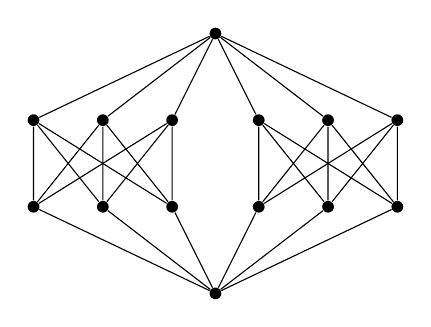
\begin{tikzpicture}[
    scale=1.1,
    every node/.style={circle,fill=black,inner sep=1.5pt}
]

\node (0) at (0,0) {};
\node (1) at (0,3) {};

\node (a1) at (-2.1,1) {};
\node (a2) at (-1.3,1) {};
\node (a3) at (-0.5,1) {};

\node (A23) at (-2.1,2) {}; % {2,3}
\node (A13) at (-1.3,2) {}; % {1,3}
\node (A12) at (-0.5,2) {}; % {1,2}

\node (b1) at (0.5,1) {};
\node (b2) at (1.3,1) {};
\node (b3) at (2.1,1) {};

\node (B23) at (0.5,2) {};
\node (B13) at (1.3,2) {};
\node (B12) at (2.1,2) {};

\draw (0) -- (a1) -- (A23) -- (1);
\draw (0) -- (a2) -- (A13) -- (1);
\draw (0) -- (a3) -- (A12) -- (1);

\draw (a1) -- (A13);
\draw (a1) -- (A12);
\draw (a2) -- (A23);
\draw (a2) -- (A12);
\draw (a3) -- (A23);
\draw (a3) -- (A13);

\draw (0) -- (b1) -- (B23) -- (1);
\draw (0) -- (b2) -- (B13) -- (1);
\draw (0) -- (b3) -- (B12) -- (1);

\draw (b1) -- (B13);
\draw (b1) -- (B12);
\draw (b2) -- (B23);
\draw (b2) -- (B12);
\draw (b3) -- (B23);
\draw (b3) -- (B13);

\end{tikzpicture}
\caption{$B_3 \oplus B_3$}
\end{figure}

Geometrically, this lattice can be interpreted as like the star of David (consider the two triangular faces to be one $2$-face, which is $\hat 1$ here.)
\end{solution}

\item Prove directly (i.e., without using polarity) that every face of a polytope $P$ is contained in a facet.

\begin{proof}
Consider the face lattice $L(P)$ (recall it is ordered by inclusion). By Theorem 2.7 it is coatomic and thus we are done. Alternatively, consider the maximal chain which contains the lattice element corresponding to the face. By Theorem 2.7 $L(P)$ must be graded of length $\dim(P) + 1$, which means that there must be a facet element in this chain, and thus we are done.
\end{proof}

\item If two $0/1$-polytopes are combinatorially equivalent, does it follow that they are affinely isomorphic? (The answer is “no.”)

\begin{solution}
First recall that a $0/1$-polytope is the convex hull of a subset of the vertices of a $d$-cube.

The answer is no. Fix the bottom triangle $(0,0,0), (1,0,0), (0,1,0)$ and pick between $(1,0,0)$ or $(1,1,1)$. Both are tetrahedrons but not affinely isomorphic to each other because parallelism differs.
\end{solution}

\item Let $f(d)$ be the number of combinatorial equivalence classes of $d$-dimensional $0/1$-polytopes. The first values are
$f(0)=f(1)=1$, $f(2)=2$, and $f(3)=8$. Prove that
\[2^{2^{d-2}} < f(d) < 2^{2^{d}} \quad \text{for } d>5.\]
(This solves a problem of Billera \& Sarangarajan [76, Sect. 3]. For the lower bound A.~Sarangarajan and I suggest that you consider all the polytopes of the form $P = \operatorname{conv}(S)$ for sets $S \subseteq \{0,1\}^d$ that satisfy
\begin{flalign*}
& \bi{x} \in S \text{ for all } \bi{x} \in \{0,1\}^d \text{ with } x_d = 1, \\
& \textbf{0},\, \textbf{1} - \bi{e}_d \in S, \; \text{and} \; \bi{e}_1,\, \textbf{1} - \bi{e}_d - \bi{e}_1 \notin S.
\end{flalign*}
There are $2^{2^{d-1}-4}$ such polytopes $P(S)$; show that their combinatorial equivalence classes are “small.”)

\begin{proof}
We first prove the upper bound $f(d) < 2^{2^d}$. Indeed, for a $d$-dimensional $0/1$-polytope, it can have at most $2^d$ vertices (combinatorially equivalent to a subset of vertices in the $d$-cube). This amounts to $2^{(2^d)}$ choices for its vertex set. The strict inequality follows because not every choice of vertices generates a $d$-dimensional convex hull (for example, the trivial polytope, from picking exactly none of the points).

Following Sarangarajan and Ziegler's suggestion, we consider the suggested polytopes for the lower bound. There are exactly $2^{2^{d-1}}$ $d$-dimensional polytopes with every vertex having $x_d = 1$, and then the four further restrictions give the desired count of $2^{2^{d-1}-4}$ such polytopes. 

\ermactually{count the equivalence classes bru}
\end{proof}

\item Assume that one is given the vertex–facet incidence matrix 
\[ M(P) \in \{0,1\}^{m\times n} \equiv \{\cdot,\ast\}^{m\times n} \]
of a convex polytope $P$ with $m$ vertices and $n$ facets.

How can the face lattice of the polytope $P$ be uniquely reconstructed from the knowledge of $M(P)$ alone? How does the dimension of $P$ appear in the computation? How does your algorithm fail if the matrix you apply it to is not the vertex–facet matrix of a polytope? What is the relation between the matrices of $P$ and $P^\Delta$?

\begin{solution}
From $M(P)$ we know the vertices each facet contains. The intersection of the vertex set of a set of facets is either empty or a lower dimensional face. To be explicit, let $E$ be the set of facets (i.e. columns of $M(P)$) and let $S \in 2^E$ cycle through all the subsets of $E$. We compute

\[V(S) =  \bigcap_{F \in S}\textup{vert}(F)\]

and keep the nonempty $V(S)$. Because the face lattice of a polytope is coatomic, this multi-intersection finds every face. We can then simply partially order the faces by inclusion to recover the face lattice.

Once we have the lattice, $\dim(P)+1$ is simply the length of any maximal chain (the lattice is graded so any maximal chain works).

If $M$ is not a vertex-facet incidence matrix for some polytope, the resulting lattice will not satisfy Theorem 2.7, or it will be of block form under relabeling (i.e. $F = F_1 \sqcup F_2, f_1 \cap f_2 = \varnothing$ for all $f_1 \in F_1, f_2 \in F_2$).

Lastly, we have that $M(P^{\Delta}) = M(P)^\intercal$.
\end{solution}

\item Let $P$ and $P'$ be polytopes with vertex sets $V = \{v_1,\dots,v_n\}$ and $V' = \{v_1',\dots,v_n'\}$. Assume that for every vertex set $F \subseteq V$ of a facet of $P$, the corresponding set $F' \subseteq V'$ is the vertex set of a facet of $P'$. 
\begin{enumerate}[label=(\roman*)] 
\item Show that for every face of $P$, the corresponding vertex set of $P'$ forms a face in $P'$. Deduce that $\dim(P) \le \dim(P')$. 

\item Lemma if $P$ and $P'$ have the same dimension, then they are combinatorially equivalent under $v_i \to v_i'$. (Hint: Assume this fails. Then $P'$ has two facets, $F_1'$ and $F_2'$, which are adjacent, such that of the corresponding vertex sets in $P$, the set $F_1$ forms a facet, but $F_2$ does not. (Here you can use the fact that the graph of $(P')^\Delta$ is connected: a proof is in the next lecture.) Now consider the ridge $F_1' \cap F_2'$, which is a facet of $F_1'$, and use induction on the dimension, applied to the polytopes $F_1$ and $F_1'$.) 

\item Show that $P$ and $P'$ need not have the same dimension. (Hint: For this, one can take a cube $P = C_3$, labeled as in the drawing, and a cyclic polytope $P' = C_4(8)$.)

\item Assume that of a polytope $P$ you are given the dimension, the vertex set, and a matrix $M(P) \in \{0,1\}^{m\times n}$ such that every row of $M(P)$ represents a facet of $P$. 

How can you tell whether this list of facets is complete? (Remark: this is not too easy; one can use tools from Chapter~8, or from homology theory.) 

(Part (ii) is important: See Klee \& Minty [330, p.~167], Amenta \& Ziegler [17], and elsewhere. (iii) points to an error in [330, p.~167].)
\end{enumerate} 
\begin{solution}
\begin{enumerate}[label=(\roman*)] 
    \item We get that the columns of $M(P)$ is a subset of the columns of $M(P')$. The claim follows by applying the procedure outlined in Exercise 2.7

    \item Assume $\dim(P) = \dim(P')$ but $M(P) \neq M(P')$. Thus there exists adjacent two facets $F_1', F_2'$ in $P'$ where the corresponding $F_1 \in P$ forms a facet, but $F_2$ doesn't. Consider the ridge formed by $F_1' \cap F_2'$, which is a facet for $F_1'$. Notice $\dim(F_1') = \dim(F_1) = \dim(P)-1$, so we can simply induct on the dimension of the polytope. The base case is trivial and thus we are done.

    \item Consider $C_3$, the $3$-cube, and $C_4(8)$, a cyclic polytope. The facets of $C_4(8)$ are, by Gale's evenness condition
    \[\{1234,1245,1256,1267,1278,2345,2356,2367,2378,\]
    \[3456,3467,3478,4567,4578,5678,1238,1348,1458,1468,1678 \}\]

    Following Ziegler's suggest labeling of $C_3$, its facets are
    \[\{1234, 1278, 2367, 3456,1458, 5678\}\]

    and one sees that the facets of $C_3$ are a subset of the facets of $C_4(8)$. The fact that $\dim(C_3) = 3 < 4 = \dim(C_4(8))$ concludes the proof.

    \item We will save this for later, either after chapter 8 or when I learn some homotopy theory.

    \ermactually{one day...}
\end{enumerate} 
\end{solution}

\item Define the \emph{face figure} $P/F$ for any face of $P$ by $ P/F := (F^\diamond)^\Delta$, that is, a polar of the face of $P^\Delta$ which corresponds to $F$. (The face figures $P/F$ are also known as the \emph{quotients} of $P$. Thus a quotient of $P$ is the same thing as an iterated vertex figure.) Show that this is a polytope of dimension 
\[ \dim(P/F) = \dim(P) - \dim(F) - 1. \] 
Characterize the face lattice of a face figure in terms of the face lattice of $P$ and of the element $F \in L(P)$. Describe a more direct construction of $P/F$, generalizing the case of a vertex figure. How can the face figure $P/F$ be obtained as an iterated vertex figure?

\begin{solution}
    We know that $k$-faces in $P$ correspond to $\dim(P) - k - 1$-faces in $P^{\Delta}$, because $L(P^\Delta) = L(P)^{op}$ (Corollary 2.14). Thus $\dim(P/F) = \dim(P) - \dim(F) - 1$. The lattice of the face figure is simply $L(P/F) = L(F^\diamond)^{op} = [F, \hat1] = [F,P]$ in the original lattice $L(P)$. $P/F$ essentially replaces the $k$-face $F$ with a $0$-dimensional vertex, whereas a vertex figure sends a $k$-face in $P$ to a $k-1$-face in $P/\bi{v}$. Thus, we can also interpret $P/F$ as $k+1$ iterated vertex figures. This is equivalent to iterating vertex figures on $k+1$ mutually linearly independent vertices in $F$.
\end{solution}

\item In conditions (iii) and (iv) of the characterization of the interior of a polytope (Lemma~2.8), can we assume the $x_i$ to be vertices?

\begin{solution}
    For (iii) we can. In fact, this comes directly from the fact that $P = \conv(\textup{vert}(P))$. For (iv), however, we cannot.
\end{solution}

\item Show that if $\{v_1,\ldots,v_k\} \subseteq \mathrm{vert}(P)$ is a set of vertices of $P$, then $F = \{v_1\} \vee \cdots \vee \{v_k\}$ holds in $L(P)$ if and only if $\frac{1}{k}\sum_{i=1}^k v_i \in \operatorname{relint}(F)$. Generalize to get a formula for the join of a set of faces $\{G_1,\ldots,G_k\} \subseteq L(P)$.

\begin{proof}
First let $F = \{v_1\} \vee \cdots \vee \{v_k\}$. Now assume by contradiction $\frac{1}{k}\sum_{i=1}^k v_i \notin \operatorname{relint}(F)$. Recall we have $P = \bigsqcup_{F \in L(P)}\operatorname{relint}(P)$, so it must be in the interior of some other face $F' \neq F$, which then means $\{v_1\} \vee \cdots \vee \{v_k\} = F'$, a contradiction. The converse is similar and immediate.

Generally, write $V_i$ as a set of vertices in $G_i$, $1 \leq i \leq k$ and $\Lambda := |\bigcup_{i=1}^k V_i|$. Then we have that $F = \bigvee_{i=1}^k G_i = \bigvee_{i = 1}^k V_i$ if and only if $\frac{1}{\Lambda}\sum_{i=1}^k \sum_{ v\in V_i} v \in \operatorname{relint}(F)$.
\end{proof}

\item Compute directly that every polar of a simplex is a simplex

\begin{solution}
We know that a $d-1$-simplex has exactly $\binom{d}{d-k}$ $k-1$-faces. The binomial identity $\binom{n}{k} = \binom{n}{n-k}$ combined with $L(P^\Delta) = L(P)^{op}$ (Corollary 2.14) gives the desired result.

Alternatively, we can also argue that a simplex is both simple and simplicial, which are polar, and thus its polar must also be simplicial and simple, which by exercise 0.1 means that it must be a simplex or an $n$-gon. A direct verification for the $2$-simplex (triangle) completes the proof.

\begin{remark}
    One can also use the $\mathcal{H}$-definition of a polytope (via the halfspace inequalities) to directly compute the polar polytope. For a facet $F \in \Delta_{d-1}$ with $\textup{vert}(F) \in \binom{[d]}{d-1}$, we can naturally label the vertex $F^\diamond \in P^{\Delta}$ by the singleton $[d] \setminus \textup{vert}(F)$. We wont go through with the computation here.
\end{remark}
\end{solution}

\item Define the polar of a cone by 
\[C^\Delta := \{\bi{c} \in (\mathbb{R}^d)^* : \bi{cx} \le 0 \text{ for all } \bi{x} \in C \}.\] 
Show that this definition (with ``0'' instead of ``1'') is a special case of our definition for arbitrary subsets. Formulate and prove the analogs of our Theorems~2.11 and~2.12.

\begin{solution}
The original definition of a \textit{polar set} is Definition 2.10, where the condition is $\bi{cx} \leq 1$. Because the cone is a non-negative combination of its generating vectors, it follows that $\bi{x} \in C$ means $t\bi{x} \in C, t \in \mathbb{R}_{\geq 0}$. Thus no $\bi{c} \in (\mathbb{R}^d)^*$ with $\bi{cx} > 0$ can satisfy the requirement, which is why we have $\bi{cx} \leq 0$ for the definition of the polar of a cone.

Theorem 2.11 lists the properties of the polar and the double polar. For cones, we have

\textit{Theorem. }(Polar and double-polar cones)
\begin{enumerate}[label=(\roman*)]
    \item $C \subseteq D$ implies $C^\Delta \supseteq D^\Delta$ and $C^{\Delta\Delta} \subseteq D^{\Delta\Delta}$,
    \item $C \subseteq C^{\Delta\Delta}$,
    \item $C^\Delta$ and $C^{\Delta\Delta}$ are conical,
    \item $\mathds{O} \in C^\Delta$ and $\textbf{0} \in C^{\Delta\Delta}$,
    \item if $C$ is a cone and $\textbf{0} \in C$, then $C = C^{\Delta\Delta}$,
    \item if a cone $C$ with $\textbf{0} \in \interior(C)$ is given by $C = \cone(V)$, then
    \[C^\Delta = \{\bi{c}: \bi{c}V \leq \mathds{O}\},\]
    \item if a cone $C$ with $\textbf{0} \in \interior(C)$ is given by $C = C(A, \textbf{0})$, then
    \[C^\Delta = \{cA: \bi{c}\textbf{1} = 1\}\]
\end{enumerate} 
\begin{proof}
    Similar to the proof of Theorem 2.11, parts (i) - (iv) is pretty immediate (just working with definitions here, recall that $C^{\Delta\Delta} = (C^\Delta)^\Delta$). Write $V = V(C)$ as a generating set of vectors for the cone. (i) follows from the fact that $V(C) \subseteq V(D)$, so every $\bi{c} \in (\mathbb{R}^d)^*$ that satisfies $D$ must also satisfy $C$. (ii) comes from that $\bi{cx} \leq 0$ implies $\bi{x}^\trans\bi{c}^\trans = (\bi{cx})^\trans \leq 0$. If $\bi{c} \in C^\Delta$, then we must have $\bi{cv}_i \leq 0$ for every $v_i \in V(C)$. This means any non-negative combination $\sum\lambda_k\bi{c}_k, \; \lambda_k \geq 0$ also satisfies $\left(\sum\lambda_k\bi{c}_k\right)\bi{v}_i \leq 0$, and thus $C^\Delta$ is conical, proving (iii). (iv) is immediate. 
    
    Now, (v) follows from the earlier line of reasoning that $\bi{cx} \leq 0$ implies $\bi{x}^\trans\bi{c}^\trans = (\bi{cx})^\trans \leq 0$, which becomes a bi-conditional. For (vi) we show that 
    \[\{\bi{c}: \bi{cx} \leq 0 \textup{ for all }\bi{x}\in C\} = \{\bi{c}: \bi{cv} \leq 0 \textup{ for all }\bi{v}\in V(C)\}\]
    Which is immediate because on one hand $V(C) \subseteq C$ and on the other hand $\bi{cv} \leq 0$ for all $\bi{v}\in V$ means $\bi{cx} = \bi{c}\left(\sum\lambda_i\bi{v}_i\right)= \sum\lambda_i\bi{cv}_i \leq 0$.

    For (vii)
    \ermactually{idk ill do it later, the statement of (vii) could be wrong too xd. seems like i wanna use FL II or something}
\end{proof}
\end{solution}

\item Let $P$ be a $d$-polytope in $\mathbb{R}^d$, given by the system \[
P = P(A,\bi{z}).
\] An inequality in this system is called \emph{redundant} if deleting it from the inequality system $A \bi{x} \le \bi{z}$ does not change the polyhedron; otherwise the inequality is called \emph{irredundant}.
\begin{enumerate}[label=(\roman*)] 

\item Derive from Farkas lemma~III that an inequality is redundant if and only if it can be written as a positive combination of other inequalities in the system.

\item Derive from a Farkas lemma that if $P = P(A,\bi{z}) \ne \emptyset$ and if none of the inequalities of a system $A \bi{x} \le \bi{z}$ is redundant, then each of them defines a facet. Thus, every polytope is the intersection of its facet-defining inequalities.

\item Show that if $\bi{x}_F \in \operatorname{relint}(F)$ is a point in the relative interior of a facet $F \in L(P)$, then the inequality $\bi{ax} \le z$ defines the facet $F$ if and only if it is valid for $P$, and $\bi{ax}_F = z$.

\item Show that for every facet $F$ of $P$, there is a unique inequality $\bi{ax} \le z$ which defines $F$, and for which $\sum_{i=1}^d |a_i| = 1$.
\end{enumerate}

Together, these statements prove that any irredundant description of a $d$-polytope $P \subseteq \mathbb{R}^d$ as an $\mathcal{H}$-polytope contains exactly one inequality for each facet of $P$. Show that this statement could also be derived by polarization of Proposition~2.2. What happens in the situation when $\dim(P) < d$? How much of the uniqueness statement in part~(iii) can you rescue?

\begin{solution}
\begin{enumerate}[label=(\roman*)]
    \item Assume an inequality can be written as a positive combination. Let this inequality be the row $\bi{a}_0 \in A$, where we can write $\bi{a}_0 = \sum \lambda_i\bi{a}_i, \; \lambda_i \geq 0$ of other rows $\bi{a}_i \in A$, and the corresponding value $z_0 \geq \sum\lambda_i z_i$. Write $A'$ as deleting the row $\bi{a}_0$ from $A$, and $\bi{z}'$ as deleting $z_0$ from $\bi{z}$. We thus have, for $\bi{c} \in (\mathbb{R}^d)^* = (\lambda_1, \ldots, \lambda_d) \geq \mathds{O}$,

    \[\bi{a}_0 = \bi{c}A', \; z_0 \geq \bi{cz}'\]

    Applying FL III, we get that $\bi{a}_0\bi{x} \leq z_0$ is valid for all $\bi{x} \in \mathbb{R}^d$ where $A'\bi{x} \leq \bi{z}'$, thus it is redundant. The converse follows because FL III is a biconditional.

    \item We use FL III again. Note that since $P \neq \varnothing$, case (ii) is impossible. For all the irredundant inequalities, we have $\bi{c}A = \bi{a}_0$, and it is important that $\bi{a}_0$ here is in $(\mathbb{R}^d)^*$. This is because it defines a $d-1$-dimensional hyperplane, which intersects $P$ at some $d-1$ portion (not smaller, as they are all irredundant) which is exactly a facet. These facet intersections are also unique by irredundancy. The second part of the claim follows immediately.

    \item First let the inequality define the facet $F$. Then we have that the equality $\bi{ax}= z$ is the hyperplane $H$ such that $H \cap P = F$, and $\bi{ax} \leq z$ for all $\bi{x} \in P$. It immediately follows that $\bi{ax}_F = z$. Now assume $\bi{ax} \leq z$ is valid for $P$ and $\bi{ax}_F = z$. Then we have $\dim(F) = \dim(P) - 1$. Now define $G$ as $ P \cap \{\bi{x}: \bi{ax} = z\}$. Assume by contradiction that $F \not \subseteq G$, then there must be some $\bi{x}_F' \in F$ such that $\bi{ax}_F' < z$. But then $\dim(G) < d-1$, which means it is redundant by (ii) (because it is not a facet-defining inequality). It follows that $F \subseteq G$, and in fact $F = G$ because $\dim(G) \leq d-1$, and $G \subseteq P$. It follows that the inequality $\bi{ax} \leq z$ is the facet-defining inequality for the facet $F$ in polytope $P$.
    
    \item Assume inequalities $I_1$ and $I_2$ both define $F \in P$. But then their equality hyperplanes must both be the affine plane of the facet $F$, with the same direction of inequality to contain $P$, and thus they are the same. Now, we can normalize the coefficients in the inequality $\bi{a} = (a_1, \ldots, a_d) \in (\mathbb{R}^d)^*$ by simply dividing them all by the norm $\sum_{i=1}^d |a_i|$.
    
\end{enumerate}
\end{solution}

\item Let $P = \operatorname{conv}(V) \subseteq \mathbb{R}^d$ be a convex $d$-polytope, and assume that some description of $P$ as an $\mathcal{H}$-polytope is known, \[ P = P(A,z). \] With every inequality $\bi{a}_i \bi{x} \le z_i$ in this system, associate its vertex set \[ V_i := \{\bi{v} \in V : \bi{a}_i \bi{v} = z_i\}. \] Show that the following criteria can be used to check whether an inequality is redundant. 

\begin{enumerate}[label=(\roman*)]
\item The inequality $\bi{a}_i \bi{x} \le z_i$ is redundant if and only if $V_i \subseteq V_j$ for some $j \neq i$. 

\item If $V_i = V_j$, then either the inequalities are multiples of each other, or they can both be deleted from the system. 

\item An inequality is irredundant if and only if it defines a facet of $P$ and no multiple of it is contained in the system. 

\item If $\lvert V_i\rvert < d$, then the inequality $\bi{a}_i \bi{x} \le z_i$ is redundant. 

\item The inequality $\bi{a}_i \bi{x} \le z_i$ is irredundant if and only if there is no multiple of it in the system, and the rank of the matrix given by $\left\{\binom{1}{\bi{v}} : \bi{v} \in V_i\right\}$ is $d$. 
\end{enumerate} 

(Parts (i) and (v) yield complete criteria for redundancy, which can be checked explicitly. Note that there was no assumption that the set $V$ has to be minimal. Condition (i) is (equivalent to) the main condition of Chernikova [149], while condition (v) is a rank test that seems not so efficient. For example, a combination of criteria (i) and (iv) makes sense in practice.) 

\begin{solution}
\begin{enumerate}[label=(\roman*)]
    \item It is clear that $V_i \subseteq V_j$ implies the inequality as redundant. Now assume that $V_i \nsubseteq V_j$ for all $j$. Write $H_i = \{\bi{a}_i\bi{v} = z_i\}$ and $F_i = P \cap H_i$. It follows that $F_i \nsubseteq F_j$ for every $j$, and thus $H_i$ is irredundant.

    \item Let $V_i = V_j$. Suppose $|V_i| = d$, then $F_i = F_j$ and $\dim(F_i) = d-1$, so $H_i = H_j$ and thus the inequalities are multiples of each other. Now suppose $|V_i| < d$, then $V_i, V_j \subseteq V(F)$, the vertex set of some facet. Then both $H_i$ and $H_j$ are redundant by Exercise 2.14 part (ii).

    \item follows from (Exercise 2.15) part (ii)

    \item follows from (Exercise 2.15) part (ii)

    \item  $\rank\begin{pmatrix}
        1 & \ldots & 1 \\ v_1 & \ldots & v_d  
    \end{pmatrix} = d$ if and only if no $\bi{v} \in V$ can be written as a convex combination of the other vertices, which is really just checking that all the $\bi{v} \in V$ are real vertices. If this is satisfied, then the $d$ vertices define a $d-1$-face of $P$, which is indeed a facet. The rest simply follows by parts (iii) and (iv).
\end{enumerate}
\end{solution}

\item Let $P = \operatorname{conv}(V) \subseteq \mathbb{R}^d$ be a convex $d$-polytope, and assume that an irredundant description of $P$ as an $\mathcal{H}$-polytope,

\[ P = P(A,z), \]

is known, such that the inequalities $\bi{a}_i \bi{x} \le z_i$ describe all the distinct facets of $P$, without duplication. For every inequality $\bi{a}_i \bi{x} \le z_i$ in the system, let $V_i$ be the set of points in $V$ which satisfy it with equality. Show that from this, an irredundant description of $\operatorname{proj}_d(P) \subseteq \mathbb{R}^{d-1}$ can be obtained from the following criteria:

\begin{enumerate}[label=(\roman*)]
\item if $a_{id} = 0$, then $\bi{a}_i \bi{x} \le z_i$ determines a facet of $\operatorname{proj}_d(P)$,
\item if $a_{id} > 0$ and $a_{jd} < 0$, then the inequality

\[ a_{id}\,\bi{a}_j + (-a_{jd})\,\bi{a}_i \;\le\; a_{id} z_j + (-a_{jd}) z_i \]

defines a facet of $\operatorname{proj}_d(P)$ if and only if $V_i \cap V_j \subseteq V_k$ holds for no $k \ne i,j$.
\end{enumerate}

Furthermore, show that if $\lvert V_i \cap V_j\rvert < d-1$, then the combined inequality in~(ii) is redundant. In particular, this is the case if $d \ge 2$ and $V_i \cap V_j = \emptyset$. (Give geometric proofs --- they are easier than algebraic ones!)

Explain how, by using Fourier--Motzkin elimination (Theorem~1.4) together with these redundancy criteria, one can obtain a complete irredundant description of $P := \operatorname{conv}(V) \subseteq \mathbb{R}^d$, even if the set $V$ contains more points than just the vertices of $P$.

How can the criterion be adapted for the case of polyhedra, where the input is a polyhedron given as $P = \operatorname{conv}(V) + \operatorname{cone}(X)$?

What happens in the situation where $\dim(P) < d$, and how can the difficulty there be overcome?

(The necessary and sufficient criterion can be found, for example, in Burger’s version [140, Thm.~3] of the double description method [416]. The test on “$V_i \cap V_j = \emptyset$” is a heuristic in Chernikova [149].)

\begin{solution}
    The outlined procedure is similar to Fourier-Motzkin. Part (i) takes care of when the inequality has no direction $x_d$ component (i.e. it is "parallel" to the $x_d$-axis), so that there is no need to change anything about the inequality. Part (ii) is the construction of the new inequalities. The rows $\bi{a}_i$ with $a_{id} > 0$ can be seen as the ones which, from the perspective of the $x_d$-axis, is on top as an upper bound for the polytope. Vice versa for the $a_{jd}<0$ inequalities, which can be rewritten as $x_d > \ldots$. If you view $\mathbb{R}^{d}$ as $1 + (d-1)$ dimensions (essentially picturing $\mathbb{R}^{d-1}$ as $\mathbb{R}$), the 2D visualization becomes clear, and then $a_{id}$ is simply the 'slope'. Here is an illustration

\begin{figure}[h]
    \centering
\begin{tikzpicture}[scale=1.5]
  \draw[->] (-1,0) -- (3,0) node[right] {$x_1, \ldots, x_{d-1}$};
  \draw[->] (0,-1.5) -- (0,2) node[above] {$x_d$};

  \draw[dashed,domain=-0.5:2.5] plot(\x,{1 - 0.5*\x});
  \draw[thick, domain=0:0.8] plot(\x,{1 - 0.5*\x});
  \draw[dashed,domain=-0.5:1.5] plot(\x,{2*\x - 1});
  \draw[thick,domain=0:0.8] plot(\x,{2*\x - 1});
  \draw[thick,domain=-0.8:0] plot(\x,{\x+1});
  \draw[thick,domain=0:0.8] plot(-\x,{3*\x/2 - 1});
  \draw[dashed,domain=-1:2] plot(0.8,\x);

  \fill (4/5,3/5) circle (1.5pt);
  \fill (4/5,0) circle (1.5pt);
\end{tikzpicture}
\caption{$\proj_d(P)$}
\end{figure}

    Geometrically, what $a_{id}\,\bi{a}_j + (-a_{jd})\,\bi{a}_i \;\le\; a_{id} z_j + (-a_{jd}) z_i$does is that, the equality is exactly the dimension $(d-1)-1 = d-2$ intersection $(H_i \cap H_j) \cap P$, projected down by $\pi: \mathbb{R}^d \to \mathbb{R}^{d-1}, \pi(x_1, \ldots, x_{d-1},  x_d) = (x_1, \ldots, x_{d-1})$. The inequality is simply in the valid direction of the projected polytope.

    The inequality is clearly true because it is a combination of true inequalities. It is also clear that the condition $V_i \cap V_j \nsubseteq V_k$ is simply checking for redundancy, as per Exercise 2.15. 

    Using Exercise 2.15 (and the fact that the projected polytope is of dimension $d-1$, it follows that if $|V_i \cap V_j| < d-1$, then the corresponding combined inequality is not a facet-defining inequality for $\proj_d(P)$ and therefore redundant. Refer to the illustrated figure for 2D intuition (think about the intersection point of the affine hull of a pair of non-adjacent edges).

    For a redundant set of vertices $V$ (i.e. not every $\bi{v} \in V$ is actually a vertex), we can perform Fourier-Motzkin in every (axial) direction and therefore eliminate all the imposters among $V$ as the elements that never show up uniquely in $\proj_k(P)$ for some direction $x_k$. Uniquely for a vertex $\bi{v}$ means that there is no other $\bi{v}' \in V$ where each time $\bi{v}$ shows up in the vertex set of some projection, so does $\bi{v}'$, and their projections are the same $\proj_k(\bi{v}) = \proj_k(\bi{v}')$. After eliminating the imposter vertices, the list of irredundant inequalities can be found by applying the redundancy criteria.

    For a polyhedra $P$ of dimension $d$, we can consider the set of independent generating vectors, which one can imagine as being the vectors in the directions of the 'edges' of the cone. Then every facet-defining inequality must be of equality for $d$ vertices or generating vectors, and of course valid for the entire polyhedra.

    If $\dim(P) < d$, it may be the case that $\proj_d(P) = \varnothing$. This can be overcome by simply finding the direction $x_k$ where $\proj_k(P) \cong P$, and repeating until we can use the proedure
\begin{remark}
    If you are looking for more than intuitive motivation, see Chapter 1.3 on Fourier-Motzkin elimination in Zigler.
\end{remark}
\end{solution}

\item Show that if $P \subseteq \mathbb{R}^d$ is a polytope with two distinct vertices $\bi{u}, \bi{v}$, then there is a projective transformation $P \longrightarrow P'$ such that the vertices $\bi{u}', \bi{v}'$ have the smallest, respectively the largest, $x_d$-coordinate among all vertices of $P'$.

\begin{solution}
    It suffices to find a point $\bi{x}$ such that the lines $\bi{ux}$ and $\bi{vx}$ intersect $P$ only at $\bi{u}$ and $\bi{v}$, respectively (like a tangent line). Consider the set of facets $F(\bi{v})$ containing $\bi{v}$ and consider the positive combinations of them, as in $\sum_{F_i \in F(\bi{v})} \lambda_iH_i, \; \lambda_i \geq 0$. By 2.16 this is a redundant inequality, and if further $\lambda_i > 0$ we get that $\sum_{F_i \in F(\bi{v})} \lambda_iH_i \cap P = \{\bi{v}\}$. For some choice of $\lambda_i$'s for each, these are both $d-1$-hyperplanes. If they are parallel we are done by simply setting $x_d$ as the (shared) normal direction of these planes, and otherwise they must intersect. It suffices to pick $\bi{x}$ in this intersection and essentially pull $x$ to infinity (in a projective geometry sense) so that $\bi{ux}$ and $\bi{vx}$ become parallel lines. Then, picking $x_d$ as the direction of the line $\bi{uv}$ suffices. 
\end{solution}

\ermactually{ran out of time. come back later}

\item Let $P \subseteq \mathbb{R}^d$ be a polytope, let $F$ be a facet of $P$, and let $\pi : \mathbb{R}^d \longrightarrow \mathbb{R}^{d-1}$ be a projection map (for example, deleting the last coordinate). By “moving a point beyond $F$ to infinity,” show that by a projective transformation $P \longrightarrow P'$, we can obtain

\[ \pi(P') = \pi(F') \quad\text{and}\quad \pi^{-1}(G') \cap P' = \pi^{-1}(G') \cap F' \]

for every proper face $G' \subset \pi(F')$.

\item Using a Farkas lemma, show that for every unbounded pointed polyhedron $P$ there is an inequality $ax \le 1$ such that

\[P' := \{x \in P : ax \le 1\}\]
is a polytope with a facet $F' := \{x \in P : ax = 1\}$, such that the $k$-faces of $F'$ correspond to the unbounded $(k+1)$-faces of $P$, and the $k$-faces of $P'$ that are not faces of $F'$ are in bijection with the $k$-faces of $P$.

Show that a polyhedron combinatorially equivalent to $P'$ can also be obtained from $P$ by taking the closure of the image of $P$ after a “nonadmissible’’ projective transformation that moves the face at infinity into $\mathbb{R}^d$.

How can this be used to study the combinatorics of pointed unbounded polyhedra in terms of “polytopes with a distinguished face’’?

\item Let $P \subseteq \mathbb{R}^d$ be a $d$-polyhedron with $n$ facets and at least two vertices, and assume that $0 \in \operatorname{int}(P)$. With $P$, associate the new polyhedron
\[
  P^o := \bigl(\operatorname{conv}(\operatorname{vert}(P^\Delta)\setminus\{\mathds{O}\})\bigr)^\Delta .
\]
Show that if $P$ is a polytope, then $\mathds{O}$ is an interior point of $P^\Delta$, and $P^o = P$.

If $P$ is unbounded, then $0$ is on the boundary of $P^\Delta$. Show that the polar, with respect to an interior point of $\operatorname{conv}(\operatorname{vert}(P^\Delta)\setminus\{0\})$, is a $d$-polytope $P^o$ with $n$ facets and with more vertices than $P$.

\item The \emph{Carathéodory curve} [142] in $\mathbb{R}^{2d}$ is given by
\[
  \mathbf{y} : \mathbb{R} \longrightarrow \mathbb{R}^{2d}, \qquad
  u \longmapsto \mathbf{y}(u) :=
  \begin{pmatrix}
    \cos(u)\\
    \sin(u)\\
    \cos(2u)\\
    \sin(2u)\\
    \vdots\\
    \cos(du)\\
    \sin(du)
  \end{pmatrix}.
\]
\begin{enumerate}
\item[(i)] Show that for $0 \le u_1 < u_2 < \dots < u_n < 2\pi$ with $n > 2d$, the convex hull
\[
  C'_{2d}(u_1,u_2,\dots,u_n) :=
  \operatorname{conv}\{\mathbf{y}(u_1),\mathbf{y}(u_2),\dots,\mathbf{y}(u_n)\}
\]
is combinatorially equivalent to the cyclic polytope $C_{2d}(n)$.
(Hint: You will find a useful hint in Grünbaum [252, p.\ 67, Ex.\ 23].)

\item[(ii)] Prove that in the case $d = 2$ the map
\[
  \begin{pmatrix}
    y_1\\ y_2\\ y_3\\ y_4
  \end{pmatrix}
  \longmapsto
  \frac{1}{3 + 4y_1 + y_3}
  \begin{pmatrix}
    2y_2 + y_4\\ 1 - y_3\\ 2y_2 - y_4\\ 3 - 4y_1 + y_3
  \end{pmatrix}
\]
is a projective transformation, which maps (the relevant part of) the Carathéodory curve to the moment curve. Conclude that for suitable real parameters $t_1 < t_2 < \dots < t_n$, the polytope $C'_4(u_1,\dots,u_n)$ is in fact projectively equivalent to the “standard’’ cyclic polytope $C_4(t_1,\dots,t_n)$ defined via the moment curve (Example 0.6).
(In fact, for general $d \ge 1$ the polytope $C'_{2d}(u_1,u_2,\dots,u_n)$ is projectively equivalent to some standard cyclic polytope $C_{2d}(t_1,\dots,t_n)$. For this one can explicitly construct a projective transformation that takes the Carathéodory curve to the moment curve, using a substitution of the type
\[
  t := \frac{1-\cos(u)}{\sin(u)} = \frac{\sin(u)}{1+\cos(u)}
\]
and some elementary trigonometric identities, such as the formulas $\sin(2t) = 2\sin(t)\cos(t)$ and $\cos(2t) = 2\cos^2(t)-1$.)
\end{enumerate}

\item For relatively prime natural numbers $p,q \in \mathbb{N}$ (i.e., numbers with no common factor), define the \emph{bicyclic polytope} $P_4(p,q,n)$ as the convex hull of the $n \ge 5$ points
\[
  \mathbf{v}_i :=
  \begin{pmatrix}
    \cos\bigl(2\pi p\frac{ i}{n}\bigr)\\
    \sin\bigl(2\pi p\frac{ i}{n}\bigr)\\
    \cos\bigl(2\pi p\frac{i}{n}\bigr)\\
    \sin\bigl(2\pi p\frac{i}{n}\bigr)
  \end{pmatrix},
  \quad 1 \le i \le n.
\]
Describe the geometry and combinatorics of these polytopes.
\begin{enumerate}
\item[(i)] What symmetries do they have? Show that all the facets of $P_4(p,q,n)$ are combinatorially equivalent.
\item[(ii)] How many facets does $P_4(p,q,n)$ have? Find the conditions on $p$, $q$, and $n$ under which $P_4(p,q,n)$ is simplicial.
\item[(iii)] Using part (i) or (ii) of the previous exercise, show that the $4$-polytopes $P_4(1,2,n)$ and $P_4\bigl(1,\frac{n-1}{2},n\bigr)$ (for odd $n$) are combinatorially equivalent to cyclic polytopes $C_4(n)$.
\end{enumerate}
(Smilansky [502, 503].)

\item Try to estimate the number of combinatorial equivalence classes of $d$-dimensional polytopes with $n$ vertices. 

(Goodman \& Pollack [235, 236], Alon [112].)

\begin{solution}
    This will be more similar to a discussion, or just a collection of ideas.

    Write $f(d, n)$ as the (actual) number of combinatorial equivalences classes $d$-dimensional polytopes with $n$ vertices. We first have $f(d, d+1) = 1$, just the simplex. The $d \leq 1$ cases are trivial and $d=2$ is quite simple as well, where we have $f(2, n) = 1$ for all $n > 2$, just the $n$-gon.

    It seems like a lattice approach (using Theorem 2.7) will be hard to provide anything beyond the crudest estimates, even though it does present combinatorial equivalence quite clearly. For one, it is hard to enumerate graded, diamond, atomic \& coatomic lattices only given the number of rank $1$ elements ($n$) and the length of the maximum chain ($d$). Also, as demonstrated in exercise 2.3, not every lattice satisfying the requirements is automatically the face lattice of a polytope. Even though the smallest such example shows up at $(d,n) = (2,6)$, we suspect that the number of 'pseudo'-polytopal lattices will increase as both $d$ and $n$ increases, with no effective way to distinguish them. There are probably better ways to proceed.

    Another approach is through the vertex-facet incidence matrix $M(P)$, as in Exercise 2.7. As we saw, this matrix completely describes all the $k$-faces of the polytope, so there is no information lost here. It would be quite helpful if the solution to Exercise 2.8 (iv) was nice, because it can be used to distinguish 'complete' matrices that actually correspond to the facets of a polytope. Given $(d,n)$ we could also bound the number of facets $f$ (an easy lower bound, but depending on $n$ the upper bound can be tricky). Some sort of recursion $f(d-1, n-k)$ could also be set up, but that would rely on knowing a formula which is in itself hard. A special case is $d=3$ where all the facets are $2$-dimensional, so their combinatorial equivalence class is uniquely determined by the number of vertices. Nevertheless, piecing this information back to the $3$-polytope isn't immediate. We will try this.

    There is the graph of a polytope $P$ denoted as $G(P)$. In general, a graph is far from enough (see the ending remarks of chapter 3). But as shown in Theorem 3.12 (Blind and Mani [108]), the combinatorial structure can be completely recovered from the graph when $P$ is \textit{simple}. In other words, isomorphic graphs imply and is implied by isomorphic face lattices. This could yield interesting investigation in the special case of simple polytopes.

    As a baby step let us analyze the equivalence classes of $f(3,n)$ for $n > 3$:

    \ermactually{top ten false promises :wiltedrose:}
    
\end{solution}
\end{enumerate}

\bigskip
\section{Graphs of Polytopes}

\begin{enumerate}
\setcounter{enumi}{-1}
\renewcommand{\labelenumi}{3.\arabic{enumi}}
\item (\textbf{Stellar subdivisions}  [204]). Let $F$ be a facet of the $d$-polytope $P \subseteq \mathbb{R}^d$, and construct a point $\bi{y}_F \in \mathbb{R}^d$ beyond $F$. The polytope

\[\operatorname{st}(P,F) := \operatorname{conv}(P \cup \{\bi{y}_F\})\]
is the \textit{stellar subdivision} of $P$ at $F$.

\begin{enumerate}[label=(\roman*)]

\item Describe the faces of $\operatorname{st}(P,F)$ in terms of faces of $P$. Conclude that the combinatorial type of $\operatorname{st}(P,F)$ does not depend on the precise position of $\bi{y}_F$.

\item Show that if $P$ is simplicial, then so is $\operatorname{st}(P,F)$. In this case, count the number of $k$-faces of $\operatorname{st}(P,F)$ in terms of the numbers $f_i(P)$ of $i$-faces of $P$.

\item Describe the operation that is “polar’’ to stellar subdivision, given by

\[\operatorname{st}^\Delta(P,\bi{v}) := \bigl(\operatorname{st}(P^\Delta,\bi{v}^\diamond)\bigr)^\Delta,\]
for any vertex $\bi{v}$ of $P$.
\end{enumerate}

\begin{remark}
    Recall that 'beyond' is defined. For visualization it may help to see $\bi{y}_F$ as $1+\epsilon$ times the barycenter of all the vertices of $F$. Of course, as we'll show, the precise position doesn't matter.
\end{remark}
\begin{solution}
\begin{enumerate}[label=(\roman*)]
\item Notice that an edge is formed between $\bi{y}_F$ and every vertex $\bi{v} \in V(F)$. Every $k$-face $S \subset F$ becomes a $k+1$-face of $\conv{(F \cup \bi{v})}$ (including the $-1$-empty face, which becomes the vertex $\bi{y}_F$), with the exception that the entire $d$ face $\conv{(F \cup \bi{v})}$ just becomes part of $\operatorname{st}(P,F)$ (along with $P$). Furthermore, by the definition of 'beyond', none of the other facets are changed and $\bi{y}_F$ forms no edges with $\bi{v}' \in V(P)\setminus V(F)$.

\item If $P$ is simplicial, then every facet $F$ is a $d-1$-simplex. Denote its vertex set $V(F) = [d]$. Then $\operatorname{st}(P, F)$ loses the facet $F$ but gains the $d$ new facets $\conv(S + \bi{y}_F)$ for all $S \in \binom{[d]}{d-1}$, which are simplexes. Thus $\operatorname{st}(P,F) $ is still simplicial. Furthermore, $f_i(\operatorname{st}(P, F)) = f_i(P) + \binom{d}{i}$ for $0 \leq i < d$, and simply $f_d(\operatorname{st}(P,F)) = f_d(P) = 1$. 
    
 \item The operation $\operatorname{st}^{\Delta}(P,\bi{v})$ essentially 'cuts' the vertex $\bi{v}$ off. Equivalently, adjoin the inequality of the hyperplane that cuts of $\bi{v}$ in the vertex figure (in the admissible direction) to the list of inequalities that define $P = P(A, \bi{z})$. Its easy to see that the structure of $P \setminus F$ is unchanged, as per (i). Then, recall that $\bi{v}^\diamond$ is a facet in $P^\Delta$ whose vertex set consists exactly of the polar of those facets in $P$ that contain $\bi{v}$. Thus we get that the original vertex $\bi{v}$ is replaced with a facet (that is the vertex figure of $\bi{v}$ in $P$) and as per (i) connectivity follows naturally.

 \ermactually{hmm do i wanna elaborate}
 
 Below is an illustration:

\begin{figure}[h]
    \centering
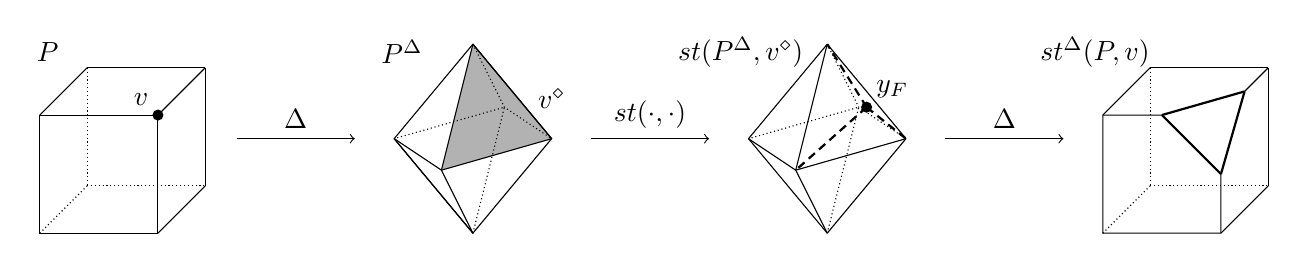
\begin{tikzpicture}[scale=1]
\coordinate (A) at (0,0.2);
\coordinate (B) at (1.5,0.2);
\coordinate (C) at (1.5,1.7);
\coordinate (D) at (0,1.7);
\coordinate (E) at (0.6,0.8);
\coordinate (F) at (2.1,0.8);
\coordinate (G) at (2.1,2.3);
\coordinate (H) at (0.6,2.3);

\draw (A) -- (B) -- (C) -- (D)--cycle;
\draw[densely dotted] (E) -- (F);
\draw (F) -- (G);
\draw (G) -- (H);
\draw[densely dotted] (H) -- (E);
\draw[densely dotted] (A) -- (E);
\draw (B) -- (F);
\draw (C) -- (G);
\draw (D) -- (H);

\fill (C) circle (2pt);
\node[above left] at (C) {$\bi{v}$};
\node[xshift = -5mm, yshift = 2mm] at (H) {$P$};

\draw[->] (2.5,1.4) -- (4,1.4) node[midway,above] {$\Delta$};

\coordinate (L)  at (4.5,1.4);
\coordinate (R)  at (6.5,1.4);
\coordinate (T)  at (5.5,2.6);
\coordinate (Bv) at (5.5,0.2);
\coordinate (Fv) at (5.9,1.8);
\coordinate (Kv) at (5.1,1.0);

\fill[black!30] (T) -- (Kv) -- (R) -- cycle;
\node[yshift = 5mm] at (R) {$\bi{v}^\diamond$};
\node[xshift = 1mm, yshift = 11mm] at (L) {$P^\Delta$};
\draw (L) -- (T) -- (R) -- (Bv)--cycle;
\draw (L) -- (Bv);
\draw (R) -- (T);
\draw[densely dotted] (T) -- (Fv) -- (R);
\draw[densely dotted] (Bv) -- (Fv) -- (L);

\draw (T) -- (Kv) -- (Bv);
\draw (L) -- (Kv) -- (R);

\draw[->] (7,1.4) -- (8.5,1.4) node[midway,above] {$\operatorname{st(\cdot, \cdot)}$};

\coordinate (L)  at (9,1.4);
\coordinate (R)  at (11,1.4);
\coordinate (T)  at (10,2.6);
\coordinate (Bv) at (10,0.2);
\coordinate (Fv) at (10.4,1.8);
\coordinate (Kv) at (9.6,1.0);
\coordinate (C) at (10.5,1.8);

\fill (C) circle (2pt);
\node[xshift = -1mm, yshift = 11mm] at (L) {$\operatorname{st}(P^\Delta, \bi{v}^\diamond)$};
\node[above right] at (C) {$\bi{y}_F$};
\draw (L) -- (T);
\draw (Bv) -- (R);
\draw (L) -- (Bv);
\draw (R) -- (T);
\draw[thick, densely dashed] (C) -- (T);
\draw[thick, densely dashed] (C) -- (Kv);
\draw[thick, densely dashed] (C) -- (R);
\draw[densely dotted] (T) -- (Fv) -- (R);
\draw[densely dotted] (Bv) -- (Fv) -- (L);

\draw (T) -- (Kv) -- (Bv);
\draw (L) -- (Kv) -- (R);

\draw[->] (11.5,1.4) -- (13,1.4) node[midway,above] {$\Delta$};

\coordinate (A) at (13.5,0.2);
\coordinate (B) at (15,0.2);
\coordinate (D) at (13.5,1.7);
\coordinate (E) at (14.1,0.8);
\coordinate (F) at (15.6,0.8);
\coordinate (G) at (15.6,2.3);
\coordinate (H) at (14.1,2.3);
\coordinate (C1) at (14.25,1.7);
\coordinate (C2) at (15,0.95);
\coordinate (C3) at (15.3,2);

\draw (A) -- (B) -- (C2) -- (C1) -- (D)--cycle;
\draw[densely dotted] (E) -- (F);
\draw (F) -- (G);
\draw (G) -- (H);
\draw[densely dotted] (H) -- (E);
\draw[densely dotted] (A) -- (E);
\draw (B) -- (F);
\draw (C3) -- (G);
\draw (D) -- (H);
\draw[thick] (C1) -- (C3);
\draw[thick] (C2) -- (C3);
\draw[thick] (C1) -- (C2);

\node[xshift = -7mm, yshift = 2mm] at (H) {$\operatorname{st}^\Delta(P, \bi{v})$};
\end{tikzpicture}

\caption{The polar stellar subdivision}
\end{figure}
\end{enumerate}
\end{solution}

\item For a vertex $\bi{v}$ of the $d$-polytope $P$, and $k \ge 1$, construct the cones generated by all vertices of $P$ of distance $k$ from $\bi{v}$:
\[C_k := \operatorname{cone}\{\bi{w}-\bi{v} : \bi{w} \in \operatorname{vert}(P), \delta(\bi{v},\bi{w}) = k\}.\]

Prove the "nested cone theorem" of Hochstättler [275]:
\[C_1 \supseteq C_2 \supseteq C_3 \supseteq \ldots\]

\begin{solution}
    WLOG assume $\bi{v} = \textbf{0}$ Assume by contradiction $C_{i+1} \nsubseteq C_i$ for some $i$. Then there exists $\bi{w}$ which is distance $k+1$ away from $\textbf{0}$ such that it cannot be written as the non-negative combination of all the distance $k$. But then that means that there exists an edge $(\bi{w}', \bi{v})$ for some $\bi{w'}$ such that $\delta(\bi{w}', \bi{v}) < k$, or, if there is none, the edge $(\textbf{0}, \bi{v})$, either of which is a contradiction.

    \begin{remark}
        The central idea here is the \textit{concavity} of the polytope.
    \end{remark}
\end{solution}

\item If $P$ has dimension at least $4$, then the graph $G(P)$ is not planar. In fact, show that it contains a subdivision of the complete graph $K_{d+1}$ (Gr\"unbaum [252, pp.~200, 214]).

\begin{solution}
    We strengthen the hypothesis to claiming that the subdivision arises from $d-1$ vertices in a facet and $1$ vertex outside the facet. The proof is by induction. The base case $d=2$ is clear, so assume that the claim is true for $d-1$. Now let $P$ be a $d$-polytope. Find two adjacent facets $F_1$ and $F_2$ (i.e. sharing a ridge $R = F_1 \cap F_2$). Now find $\bi{v} \in F_1$ and $\bi{w} \in F_2$ such that $\bi{v} \cup \operatorname{vert}(R)$ and $\bi{w} \cup \operatorname{vert}(R)$ are both subdivisions of $K_d$. Now notice that there is a path from $\bi{v}$ to $\bi{w}$ that doesn't use any vertices in $F_1$ or $F_2$, because the graph of the polytope remains connected after removing all such vertices. Thus we obtain $K_{d+1}$ and are done.
    
    \begin{remark}
        Non-planarity follows from Kuratowski's Theorem, which says that a graph is planar if and only if it does not contain the subdivision $K_5$ or $K_{3,3}$.
    \end{remark}

    \begin{remark}
        In fact, a $d$-dimensional polytope $P$ cannot contain subdivisions of complete graphs with more than $d+1$ vertices. 
    \end{remark}
\end{solution}

\item If $n > d \ge 4$, then the graph of the cyclic polytope $C_d(n)$ is complete, $G(C_d(n)) = K_n$. Give a direct proof: for each edge, construct an explicit linear function that is maximized by this edge.

\begin{solution}
    Before proceeding to the solution, here is some motivation. Recall in Exercise 0.8 we showed that cyclic polytopes $C_d(n)$ are $\lfloor \frac{d}{2} \rfloor$-neighborly. This is why $G(C_d(n)) = K_n$ is complete when $n > d \ge 4$. Alternatively, for an edge, consider all the hyperplanes for facets which contain this edge, and simply take some affine combination of the equations. The resulting equation defines a hyperplane which only intersects with the polytope at the desired edge and is a valid (redundant) inequality for the polytope, and it is the desired linear function. Of course, this is all cheating here.
    
    Directly, let the vertices be $\textbf{x}(i)$ for all $i\in [n]$. Then every edge is $(\textbf{x}(i), \textbf{x}(j))$ for some $i\neq j$, and we want to construct a linear function $\bi{c}_{ij} \in (\mathbb{R}^d)^*$ which is maximized only by this edge (and by no other vertices, essentially), for every edge. Thus, we need $\bi{c}_{ij}\textbf{x}(i) = \bi{c}_{ij}\textbf{x}(j) = \alpha$, and $\bi{c}_{ij}\textbf{x}(k) < \alpha$ for all other $k$.

    \ermactually{im gonna leave this for now. found some patterns but no general ideas yet.}
\end{solution}

\item A $d$-polytope $P$ is called \emph{dimensionally ambiguous} if there is a polytope $Q$ of a different dimension $\dim(Q) \neq \dim(P)$ which has an isomorphic graph, $G(P) \cong G(Q)$.

\begin{enumerate}[label=(\roman*)]
\item Show that the $d$-simplex is dimensionally ambiguous for $d \ge 5$, but not for $d \le 4$.

\item Show that $3$-polytopes, and simple $4$-polytopes, cannot be dimensionally ambiguous. (Hint: Use Exercise~3.2!)

\item Show that if $P$ is a $0/1$-polytope whose graph is isomorphic to $G(C_d)$, then $P$ is affinely isomorphic to $C_d$. (Compare to Exercise~2.5!)

\item Show that the $d$-cubes are dimensionally ambiguous. In particular, describe a $4$-polytope whose graph is isomorphic to $G(C_5)$! (Suitable polytopes can be constructed directly, or can be identified within Blind \& Blind's [107] classification of all cubical $d$-polytopes with $2^{d+1}$ vertices. Indeed there are cubical $4$-polytopes with the graph of the $n$-cube, for any $n \ge 4$. More generally, ``neighborly cubical polytopes exist!'' --- see Babson, Billera \& Chan [33] and Joswig \& Ziegler [294].)

\end{enumerate}

\begin{solution}
\begin{enumerate}[label=(\roman*)]
\item For $d \geq 5$ we have $G(\Delta_d) \cong G(C_{d-1}(d+1))$. For $d \leq 4$ we know that any $2$-neighborly polytope has every $3$-face as a simplex (by Exercise 0.10). This takes care of $d \leq 3$. Now since $\Delta_4$ has $5$ vertices there cannot be a higher dimensional polytope with isomorphic graphs, and yet a lower dimension $2$-neighborly polytope must be a simplex which has only $4$ vertices. Thus we are done.

\item First notice that all polytopes of dimension $\leq 2$ are simple, meaning the for any vertex $v$ we have $\deg(v) \leq 2$. So, since a $3$-polytope $P$ have vertices of degree $\geq 3$, it cannot coincide with the graph of a lower-dimensional polytope. Then, since its graph $G(P)$ is planar, by Exercise 3.2 it cannot coincide with a higher dimensional polytope. A simple $4$-polytope has $\deg(v) = 4$ for every vertex, which means it cannot coincide with a higher dimensional polytope. But its graph is contains $K_5$ which no lower dimensional polytope can contain. Thus we are done.

\item Since $C_d$ is simple, no higher dimensional polytope is graphically congruent. Assume $P$ is a $0/1$-polytope and $G(P) \cong C_d$. We proceed by induction, and the base case is trivial. Thus $P$ must have two disjoint facets $F_1$ and $F_2$ that are isomorphic to $C_{d-1}$. It suffices to show that, for a $\bi{k} \in \{0,1\}^n$ sharing no component with any $\bi{v}\in F_1$, the map $\varphi: \operatorname{vert}(F_1) \to \operatorname{vert}(F_2): \; \varphi(\bi{v}) = \bi{v}+\bi{k}$ is a bijection, because then the affine isomorphism which sends $F_1$ to $C_{d-1}$ and $\bi{k}$ to $e_d$ suffices. Assume this is not the case by contradiction, then there must be a vertex $\bi{w} \in F_2$ such that $\bi{w} - \bi{k}$ is not a vertex in $F_1$. But then $\deg(\bi{w}) > d$, because it has $d-1$ neighbors in $F_2 \cong C_{d-1}$, and now at least $2$ neighbors in the $\bi{k}$ direction (i.e. in $F_1$), which is a contradiction. Thus we are done.

\item 

\ermactually{wat the sigma}

\begin{remark}
    In part (iv) Ziegler means the $d$-cubes, with $d \geq 5$. In part (ii) we show that lower dimensional cubes are not ambiguous ($d$-cubes are simple polytopes). 
\end{remark}

\end{enumerate}
\end{solution}

\item If $P = P(A,\textbf{1})$ is an irredundant description, show that for small enough $\lambda > 0$ the polytope

\[P' := P(A,\textbf{1}^{(\lambda)}),\]
with $\textbf{1}^{(\lambda)}_i = 1 + \lambda^i$ as in Lemma~3.2, is a simple polytope whose facets are in natural bijection with the facets of $P$. Furthermore, show that then $\delta(G(P')) \ge \delta(G(P))$; thus it is sufficient to prove the Hirsch conjecture for simple polytopes.

\begin{proof}
    Consider the facet hyperplanes. For a $d$-polytope $P$ and a $\bi{v} \in \operatorname{vert}(P)$, $\deg(\bi{v})$ is the number of hyperplanes that intersect at $\bi{v}$. Adjusting by $\textbf{x}(\lambda) = \begin{pmatrix}
        \lambda \\ \lambda^2 \\ \ldots \\ \lambda^d
    \end{pmatrix}$ shifts each facets such that all the non-simple vertices become simple. We can take $\lambda$ to be a small enough amount such that every set of $d+1$ hyperplanes is disjoint (i.e. no new abundant intersections arise). The bijection of facets of $P$ and $P'$ follows naturally from their $\mathcal{H}$-descriptions. Now for two corresponding vertices $\bi{v}$ in $P$ with $\bi{v}'$ in $P'$, write $F(\bi{v})$ as the set of facets that contain $\bi{v}$. We have $F(\bi{v}) \supseteq F(\bi{v}')$, which means the set of neighbors of $\bi{v}$ is a superset of the set of neighbors of $\bi{v}'$. Since no vertices are deleted, it follows that $\delta(G(P')) \ge \delta(G(P))$, meaning it suffices to prove the Hirsch conjecture for simple polytopes.
\end{proof}

\item If $P$ is a pointed polyhedron in $\mathbb{R}^3$, show that the graph of all bounded edges is connected. Show that it is not $2$-connected in general. What about higher dimensions?

\begin{solution}
Recall that a \textit{pointed} polyhedra $P$ is such that $\lineal(P) = \{\textbf{0}\}$, or equivalently that it does not contain a 'line'. If the graph of bounded edges $G(P)$ is disconnected, $P$ must contain a line of separation, which then means $\lineal(P) \neq \{\textbf{0}\}$, a contradiction. Write $P = \conv(V) + \cone(Y)$. If $\dim(\conv(V)) = 1$ we clearly don't have 2-connectedness. If $\dim(\conv(V)) = 2$ and $\dim(\cone(Y)) \leq 1$, and furthermore that the vector $Y$ is orthogonal to the affine plane of the polytope $\conv(V)$, $G(P)$ is 2-connected. Of course if $\dim(\conv(V)) = 3$ and $\dim(\cone(Y)) \leq 1$, $G(P)$ is 2-connected as well. Otherwise $G(P)$ is only connected.

In general the number of (orthogonal) directions for which $\conv(V)$ is orthogonal to the cone $\cone(Y)$ determines the 'dimension' of $G(P)$, which by Balinski's theorem gives $d$-connectedness.

\begin{remark}
    I wonder if a $d$-connected graph can always be realized as a $d$-polytope...
\end{remark}
\end{solution}

\item Let $P \subseteq \mathbb{R}^d$ be a $d$-polytope with $2d$ facets, such that the facets containing $\bi{v} = 0$ determine the positive orthant $\bi{u} \ge 0$. Show that the facets of $P$ can have $2d-1$ facets each, if $d \ge 4$. (This is why it is hard to use inductive arguments for the $d$-step conjecture.)

\begin{solution}
\ermactually{this question is confusing}    
\end{solution}

\item Prove the following theorem by Kleinschmidt \& Onn~[336]: if $P$ is a $d$-polytope whose vertex set is contained in $\{0,1,\ldots,k\}^d$, then the diameter of its graph is bounded by
\[\delta(G(P)) \le kd.\]
Why can't this be used to get effective bounds for the diameters of $d$-polytopes? (See Problem 4.16* and Section 6.5(a) for answers.)

\begin{proof}
    It suffices to show that the distance between $\textbf{0}$ and $k\textbf{1}$ is at most $kd$, because if the inequality fails for two other points it will also fail for these two. But then, starting at $\textbf{0}$, clearly there is always an edge that increases at least one component by $1$ (and does not decrease the other components). The bound follows easily.

    \ermactually{pretty sure this is very wrong}
\end{proof}

\item Consider the simplex algorithm, applied to a linear function $\bi{c}$ on a simple, $d$-dimensional polyhedron with at most $n$ facets, such that there is a unique optimal vertex.

\begin{enumerate}[label=(\roman*)]
\item* The \textsc{edge-random} rule moves along random increasing edges, where at any given vertex the increasing edges leaving it are taken with equal probability. Can you give any subexponential upper bound (in $n$ and $d$) for the expected number of steps of this rule on any linear programming problem? Is there a polynomial upper bound?

\item[(ii)] Assume that we use the following \textsc{random-facet} pivot rule to choose the increasing edge. That is, at the starting vertex $\bi{v}$,

\begin{itemize}
\item if $\text{up-degree}(\bi{v}) = 0$, then \textsc{stop} --- the current vertex is optimal,
\item if $\text{up-degree}(\bi{v}) = 1$, then take the unique increasing edge,
\item if $\text{up-degree}(\bi{v}) > 1$, then take a random facet among facets that contain $\bi{v}$, restrict the linear program to that facet, and solve the restriction by a recursive call to \textsc{random-facet}.
\end{itemize}

(This is what Kalai in [306] calls an ``antipivot rule,'' or the ``bureaucratic'' rule.)

Show that the maximal expected running time of this algorithm can be bounded by a function $E(d,n)$, which for $n>d$ satisfies the recursion
\[
E(d,n) \le \max\left\{ 1 + E(d,n-1),\; E(d-1,n-1) + \frac{1}{d} \sum_{i=1}^{\max\{d,n-d\}} E(d,n-i) \right\}.
\]

(These recursions are in fact not hard to see; the derivation of the asymptotics implied by this recursion, $E(n,d) \le n^{4\sqrt{d}}$, is not that easy (i.e., difficult). See Matou\v{s}ek, Sharir \& Welzl [383] for a careful treatment of the asymptotic analysis.)

(Both rules are studied in G\"artner, Henk \& Ziegler [219]. In particular, for special linear programming problems it is shown that there are starting vertices for which the expected number of steps is (nearly) quadratic. See also [306].)
\end{enumerate}

\begin{solution}
\begin{enumerate}[label=(\roman*)]

    \item See \cite{Gaertner2002RandomFacet} for a sub-exponential bound.

    \item If up-degree$(\bi{v}) = 0$ we are immediately done. If up-degree$(\bi{v}) = 1$, then we take a step to move to the new vertex $\bi{w}$ through the unique increasing edge. Since there exists at least one facet $F$ such that $\bi{v} \in F$ and $\bi{w} \notin F$, we get the recursion $E(d,n) \leq 1+E(d, n-1)$. Now if up-degree$(\bi{v}) > 1$, we know that any facet containing $\bi{v}$ will contain at least one up-degree edge, because it cannot contain more than one edge from $\bi{v}$ (since $P$ is simple). Now, because $P$ is simple, there are exactly $d$ facets which contain $\bi{v}$. Each facet eliminates from $1$ up to $\max\{d, n-d\}$ facets. Summing across all facets chosen with equal probability $\frac{1}{d}$ (and notice that the true facet eliminations must be a parking function on $(1,2,\max\{d, n-d\})$), we get the upper bound $ \frac{1}{d} \sum_{i=1}^{\max\{d,n-d\}} E(d,n-i)$. Here we cannot get rid of terms because it is not immediate whether $E(d, k)$ or $E(d,k+1)$ is bigger. Of course, we still have to perform \textsc{random-facet} on the randomly selected facet $F$, which is of dimension $d-1$ and has no more than $n-1$ facets, because the facets of $F$ are in bijection with $F \cap F_i$ for all the other facets $F_i \in P$, of which there are $n-1$. Thus we obtain the term $E(d-1, n-1)$. Adding the terms up and choosing the maximum between up-degree($\bi{v}$) $= 1$ and up-degree($\bi{v}$) $>1$, we obtain the desired bound. 
\end{enumerate}
\end{solution}

\item \textbf{(Basis version of linear programming).} Let $P = P(A,\bi{z}) \subseteq \mathbb{R}^d$, and let $\bi{cx}$ be a linear function on $\mathbb{R}^d$. A subset of $d$ of the inequalities of $P$, say $A'\bi{x} \le \bi{z}'$, is a \emph{basis} if $A'$ has rank $d$ (equivalently, $A'\bi{x} = \bi{z}'$ has a unique solution $x \in \mathbb{R}^d$). A basis $A'\bi{x} \le \bi{z}'$ is \emph{feasible} if the unique solution of $A'\bi{x} = \bi{z}'$ satisfies $\bi{x} \in P$, and \emph{dual feasible} if it maximizes $\bi{cx}$ over $\{\bi{x} \in \mathbb{R}^d : A'\bi{x} \le \bi{z}'\}$ (equivalently, if $\textbf{0}$ maximizes $\bi{cx}$ over $\{\bi{x} \in \mathbb{R}^d : A'\bi{x} \le \textbf{0}\}$).

\begin{enumerate}[label=(\roman*)]
\item If $\bi{v}$ is a vertex of $P \subseteq \mathbb{R}^d$, show (using Carath\'eodory's Theorem 1.15) that there is a feasible basis that has $\bi{v}$ as its solution. If $P$ is simple, the basis is unique.

\item Show that all the feasible bases for a vertex of $P$ are connected by sequences of single-element exchanges; that is, in every such exchange one inequality from the system $A'\bi{x} \le \bi{z}'$ is replaced by a single different one from the big system $A\bi{x} \le \bi{z}$.

\item If $E$ is an edge of $P$ adjacent to $\bi{v}$, show that there is a feasible basis for $\bi{v}$ such that all but one of the inequalities $A'\bi{x} \le \bi{z}'$ are satisfied on $E$ with equality.

\item Show that if a basis is both feasible and dual feasible, then it is an optimal solution for the program $\max \bi{cx}$, $A\bi{x} \le \bi{z}$.

\item Use a Farkas lemma to prove that if $P$ is a nonempty polytope, then there is a basis that is both feasible and dual feasible.
\end{enumerate}

\begin{solution}
\begin{enumerate}[label=(\roman*)]
    \item The basis for $\bi{v}$ is simply a subset of the facets whose intersection contain $\bi{v}$ and nothing else. This always exists because for any two vertices $\bi{v}, \bi{w} \in P$, there exists a facet $F$ such that $\bi{v} \in F$ and $\bi{w} \notin F$. Such a subset is clearly feasible because $\bi{v} \in P$. Since the vertex figure of $\bi{v}$ in a simple polytope is a simplex, any subset of size less than $d$ must have intersection more than $\bi{v}$. The unique feasible basis for a simple polytope $P$ is exactly the collection of facets which contain $\bi{v}$.

    Alternatively, to use Carath\'eodory, consider the cone formed by the set of inequalities for the facets which contain $\bi{v}$. Because $\bi{v}$ is a vertex, this cone is full dimension in $\mathbb{R}^d$, with non-empty interior (it contains the polytope $P$). By Carath\'eodory's, a set of no more than $d$ inward normal vectors span $\bi{v}$. Of course, since we need $\rank(A') = d$, there must be at least $d$ inequalities. Thus we get that the feasible basis for a vertex in a simple polytope is unique.

    \item It suffices to show that for feasible bases $A_I, A_J \subseteq A$ with index sets $I$ and $J$, that for some different $i\in I \setminus J$ and $j\in J \setminus I$, $A_{I \cup  j  \setminus i}$ is also a feasible basis. For each facet $F_i \subseteq P$ write $V_i = \operatorname{vert}(F_i)$ as the set of vertices of the facet $F_i$. Thus we have $\bigcup_{i \in I} V_i = \{\bi{v}\}$. Namely, we know that for every other vertex $\bi{w} \neq \bi{v}$, there exists a facet $F_i$ where $\bi{w} \notin V_i$. 

    We claim that for every set $I$ for a feasible basis $A_I$, we can associate a unique facet (inequality) to an axial direction. Indeed, of both there are $d$, and this simply seen through performing $\operatorname{rref}(A_I)$. Thus we can always choose $i$ and $j$ such that $F_i$ and $F_j$ correspond to the same direction (in $A_I$ and $A_J$, respectively), which guaranteed that $A_{I \cup  j  \setminus i}$ is also a feasible basis. Thus we are done.

    \begin{remark}
        This is the bases exchange condition for a matroid. The ground set is the set of facets of $P$ containing $\bi{v}$ and the rank is $d$, as shown in part (i). Pretty cool.
    \end{remark}

    \item Let $E$ be the edge $(\bi{v}, \bi{w})$. It suffices to show that we can pick the index set $I$ of $A_I$ such that $\bi{w}$ is in all but one facet.

    
    
\end{enumerate}
\end{solution}

\item* For a $d$-dimensional polytope with $n$ facets, what is the maximal number $M(d,n)$ of vertices in a monotone path?

(This $M(d,n)$ is an upper bound on the largest number of steps in any simplex algorithm. It is known (see Klee \& Minty [330]) that $M(d,2d) \ge 2^d$, and roughly that
\[ M(d,n) \ge \left\lfloor \frac{n}{d/2} \right\rfloor^{\lfloor d/2 \rfloor}. \]
One might think that the upper bound given by the upper bound theorem could be sharp --- it is not; see Problem 8.41*! There is a suggestion by Klee \& Minty [330, p.~175] that there could be a function $\gamma$ such that $M(d,n) \le \gamma (n-d)d$.)

\item* Does every simple $4$-dimensional polytope have a Hamilton cycle? (This conjecture is due to Barnette; see [203, p.~158]. Some special cases are in Barnette \& Rosenfeld [54].)

\item* Let $P$ be a simple $4$-polytope. Is it true that every connected planar $3$-regular subgraph that does not separate $G(P)$ is the graph of a facet of $P$? (Without the planarity condition, this had been a conjecture of Perles [299], which was disproved in [263].)

\ermactually{ran out of time. will come back later to do the skipped problems \& problems remaining in the textbook}
\end{enumerate}
\bigskip
\section{Steinitz's Theorem for 3-Polytopes}

\begin{enumerate}
\setcounter{enumi}{-1}
\renewcommand{\labelenumi}{4.\arabic{enumi}}

\item Show that the complete graph $K_{5}$, and the complete bipartite graphs $K_{3,n}$, are $\Delta Y$-reducible. Considering the graphs that are $\Delta Y$-equivalent to $K_{6}$, show that $K_{n}$ is not $\Delta Y$-reducible, for $n \ge 6$, and that $K_{m,n}$ is not $\Delta Y$-reducible for $m,n \ge 4$.

\begin{solution}
\begin{figure}[h]
    \centering
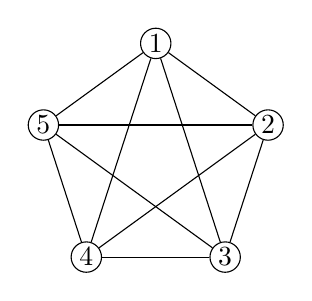
\begin{tikzpicture}[scale=1,every node/.style={circle,draw,inner sep=1pt}]
\node (1) at (90:1.5) {1};
\node (2) at (18:1.5) {2};
\node (3) at (-54:1.5) {3};
\node (4) at (-126:1.5) {4};
\node (5) at (162:1.5) {5};

\foreach \i in {1,...,5}{
  \foreach \j in {1,...,5}{
    \ifnum\i<\j
      \draw (\i) -- (\j);
    \fi
  }
}
\end{tikzpicture}

\caption{$K_5$ with labeled vertices}
\end{figure}

$K_5$ is non-planar so we cannot use Steinitz's Theorem. Instead, we will show that it is $\Delta Y$-reducible directly. Consider the following moves, labeled as "operation"(vertex set)$_{\textup{name of added vertex}}$, and $S$ means a series reduction.

\[\dy(1,2,3)_a, \dy(1,4,5)_b, S(1), \yd(4,5,a,b), \dy(3,4,a)_c, S(3), \dy(2,5,a)_d, S(2,a)\]

At this point, the remaining graph on vertex set $\{4,5,c,d\}$ is $K_4$ which we know to be $\dy$-reducible. Thus we are done.

Now we show that $K_{3,n}$ is $\dy$-reducible for all $n$. Simply perform $\yd(n,1',2',3')$ (note that $n$ is the disappearing vertex) and the resulting graph is $K_{3,n-1}$ with the extra edges $(1', 2'), (2',3'), (3',1')$, which we call $K'_{3,n-1}$. Repeatedly perform the above move and apply parallel reduction until we have no more right-hand vertices, then we are left with $K_3$ which is obviously reducible.

\begin{figure}[h]
    \centering
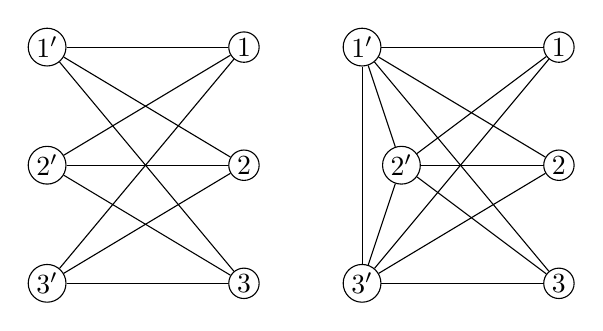
\begin{tikzpicture}[scale=1,every node/.style={circle,draw,inner sep=1pt}]
  \node (l1) at (0,1.5) {$1'$};
  \node (l2) at (0,0)   {$2'$};
  \node (l3) at (0,-1.5){$3'$};

  \node (r1) at (2.5,1.5) {$1$};
  \node (r2) at (2.5,0)   {$2$};
  \node (r3) at (2.5,-1.5){$3$};

  \foreach \i in {1,2,3}{
    \foreach \j in {1,2,3}{
      \draw (l\i) -- (r\j);
    }
  }

  \node (l1) at (4,1.5) {$1'$};
  \node (l2) at (4.5,0)   {$2'$};
  \node (l3) at (4,-1.5){$3'$};

  \node (r1) at (6.5,1.5) {$1$};
  \node (r2) at (6.5,0)   {$2$};
  \node (r3) at (6.5,-1.5){$3$};

  \foreach \i in {1,2,3}{
    \foreach \j in {1,2,3}{
      \draw (l\i) -- (r\j);
    }
  }

  \draw (l1) -- (l2);
  \draw (l1) -- (l3);
  \draw (l3) -- (l2);
\end{tikzpicture}

\caption{$K_{3,3}$ and $K'_{3,3}$ with labeled vertices.}
\end{figure}

We show that $K_6$ is not $\dy$-reducible. \ermactually{do dis}

Clearly $K_{m,n}$ for $m,n \geq 4$ is irreducible because there are no moves ($\dy, \yd, S, P$) which one can perform on it. 

\end{solution}

\item If $G$ is a $3$-connected graph with $n \ge 4$ edges, show that it contains a subdivision of $K_{4}$.

\begin{proof}
    We can assume $G$ is simple. If $G$ is planar, by Steinitz's Theorem it must correspond to a $3$-polytope, and by Exercise 3.2 we are done. If $G$ is non-planar, by Kuratowski's Theorem it must contain either a $K_5$ or a $K_{3,3}$ minor, each of which contains a $K_4$ subdivision. Thus we are done.
\end{proof}

\item Show that the definition of $k$-connectivity given in the notes to this lecture specialize to our definitions in Section 4.1 of $2$-connectivity (for graphs with more than $1$ edge) and of $3$-connectivity (for graphs with more than $3$ edges).

\begin{solution}
It suffices to show that a vertex cut of $k$ vertices is a $k$-separation. For a vertex cut, the partition of graphs $G_1$ and $G_2$ is clear, and if the $k$-vertex cut is minimal in size, both $G_1$ and $G_2$ must have more than $k$ edges, or else there exists a smaller vertex cut which is a contradiction. Furthermore, a loop allows for a $1$-separation and a parallel pair of edges allow for a $2$-separation. Thus we are done.
\end{solution}

\item What is the problem with the construction of $P$ from $P'$, if $G \to G'$ is a simple $Y$-to-$\Delta$ transformation? For this, try to prove the $Y$-to-$\Delta$ part of Lemma 4.3.

If you are comfortable with projective transformations (Section 2.6), explain how to do this without using polarity (as we did).

\begin{solution}
    Reversing the $\yd$ transformation for a polytope requires placing a vertex $\bi{v}$ beyond a facet (a 2-face of the 3-polytope, specifically) that essentially "extends" facets. Write $P' = \conv(V)$, then $P = \conv(V, \bi{v})$, and moreover let $F \in P'$ be the facet which $\bi{v}$ is beyond (i.e. $F$ separates $\bi{v}$ from $P$). Then, for a facet $F'$ adjacent to $F$ (i.e. $|\operatorname{vert}(F) \cap \operatorname{vert}(F')| = 2$), we must have that $\conv(F', \bi{v})$ is a facet in $P$. Such a position cannot always be guaranteed without having to configure the polytope $P'$
\end{solution}

\item Check how to do the reduction theorem for grid graphs entirely within the framework of $3$-connected graphs. Where are the problems? How do you make grid graphs $3$-connected? How many "basic operations" do you need?

\begin{solution}
Currently by passing to the grid graph we fall to $2$-connectability (consider the corners of the grids, for example). In order to keep the grid $3$-connected, we have to use a triangulated grid, for example with a hexagonal convex hull. We can certainly embed any planar graph as a minor of this honeycomb structure, because it contains a grid graph subdivision in it. However, performing a $\dy$ move on one of the outside triangles still loses $3$-connectability. One way to bypass this is to just bundle the moves $\dy, S, S$ into a single operation. It is easy to see that the triangular grid is indeed $\dy$-reducible under this operation.

\begin{figure}[h]
    \centering
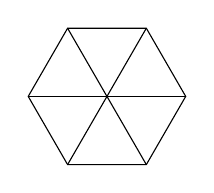
\begin{tikzpicture}[scale=1]
  \coordinate (A) at (-0.5,0.866);
  \coordinate (B) at (0.5,0.866);
  \coordinate (C) at (1,0);
  \coordinate (D) at (0.5,-0.866);
  \coordinate (E) at (-0.5,-0.866);
  \coordinate (F) at (-1,0);
  \coordinate (O) at (0,0);

  \draw (A) -- (B) -- (C) -- (D) -- (E) -- (F) -- cycle;
  \foreach \v in {A,B,C,D,E,F}
    \draw (O) -- (\v);
\end{tikzpicture}
\caption{$3$-connected triangular grid}
\end{figure}
\end{solution}

\item Characterize the graphs of centrally symmetric $3$-polytopes.
(Grünbaum [252, Thm.~13.2.5])

\begin{solution}
We claim that a graph $G = G(P)$ is realizable by a centrally symmetric $3$-polytope if and only if it is 3-connected, planar, and such that there exists an involutory mapping $\varphi$ such that all pairs of vertices $\bi{v}$ and $\varphi(\bi{v})$ are separated by a circuit in $P$.

\begin{proof}
    The 3-connected and planar requirement is simply Steinitz's Theorem. Now let $P$ be a centrally symmetric $3$-polytope. Then the desired involution is the one that sends each vertex to their corresponding symmetric counterpart through the center of symmetry. Thus it suffices to find a separating circuit. Consider all the neighbors of $\bi{v}$. Notice that $\bi{v}$ and $\varphi(\bi{v})$ cannot lie in the same facet (2-face), or else the polytope must be of less than $3$ dimensions. We claim that there must be a circuit containing the set of neighbors of $\bi{v}$, which would indeed separate $\bi{v}$ from $\varphi(\bi{v})$. Consider the set of facets containing $\bi{v}$. As it is a $2$-polytope itself, it is $2$-connected, and automatically simple. Delete $\bi{v}$ from the vertex set each facet and the remaining union of edges forms the desires separating vertex.

    Conversely, suppose that a graph $G$ has a involutory mapping on its vertices with separating circuits.
\end{proof}

\begin{figure}[h]
    \centering
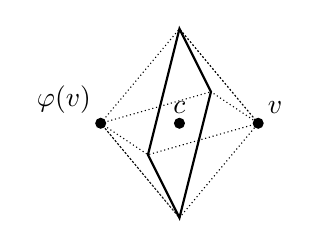
\begin{tikzpicture}
\coordinate (L)  at (4.5,1.4);
\coordinate (R)  at (6.5,1.4);
\coordinate (T)  at (5.5,2.6);
\coordinate (Bv) at (5.5,0.2);
\coordinate (Fv) at (5.9,1.8);
\coordinate (Kv) at (5.1,1.0);
\coordinate (C) at (5.5,1.4);

\node[above right] at (R) {$\bi{v}$};
\node[above left] at (L) {$\varphi(\bi{v}$)};
\fill (R) circle (2pt);
\fill (L) circle (2pt);
\node[above] at (C) {$\bi{c}$};
\fill (C) circle (2pt);
\draw[densely dotted] (L) -- (T) -- (R) -- (Bv)--cycle;
\draw[thick] (Fv) -- (T) -- (Kv) -- (Bv)--cycle;
\draw[densely dotted] (L) -- (Bv);
\draw[densely dotted] (R) -- (T);
\draw[densely dotted] (T) -- (Fv) -- (R);
\draw[densely dotted] (Bv) -- (Fv) -- (L);

\draw[densely dotted] (T) -- (Kv) -- (Bv);
\draw[densely dotted] (L) -- (Kv) -- (R);

\end{tikzpicture}
\caption{Separating circuit for an Octahedron}
\end{figure}
\end{solution}

\item Let $G$ be any finite graph drawn into the plane without crossings, and let $v$ be its number of vertices, $e$ its number of edges, $c$ its number of connected components, and $f$ the number of connected regions determined by it. Show that in general $v - e + f = 1 + c$.
Deduce \emph{Euler's formula}
\[v - e + f = 2\]
for the number of vertices $v$, the number of edges $e$, and the number of facets $f$ of a $3$-polytope.

\begin{proof}
The proof is by induction on $v+e$. One can easily check that the base case is satisfied, and now we consider all possible moves:

Placing a vertex is clearly satisfactory. Now if we connect an edge between two vertices, and a new face is made, then those two vertices were previously connected so we have not changed the number of connected components. Also, an edge cannot increase $f$ by more than $1$, thus we are good. If the edge makes no new face, then its two vertices must belong to disjoint components, and thus this edge decreases the number of connected components by one. Thus we are done.
\end{proof}

\item Deduce from Steinitz' theorem (from Corollary~4.9) that every planar graph has a straight line drawing in the plane without intersections. 

(In graph theory literature, this appears as a result of Wagner~[554], rediscovered by F\'ary~[205]. It is also quite easy to prove this directly by induction on the number of vertices; see, for example, Hartsfield \& Ringel~[273, p.~167].)

\begin{proof}
\ermactually{u want sum?}    
\end{proof}

\item Conclude from Exercise~4.6 that for every $3$-polytope $P$, either the polytope $P$ itself or its polar $P^\Delta$ has a facet that is a simplex. (This is not true for $4$-polytopes --- for these read about the regular $24$-cell, whose facets are octahedra and whose vertex figures are cubes; see, for example, Coxeter~[164, Sect.~8.2].)

\begin{proof}
    From Exercise 4.6 we have $v-e+f=2$ for a $3$-polytope $P$. Assume by contradiction that $P$ has no simplex facet (i.e. a triangle). Then we have $e \geq 2f$. Furthermore, if $\deg(\bi{v}) = 3$ for some vertex $\bi{v}$, then $\bi{v}^\diamond \in P^\Delta$ is a simplex facet. Thus we must have $\deg(\bi{v}) \geq 4$ for all vertices, which then gives $e \geq 2v$. But then we get $v-e+f \leq 0$, a contradiction.
\end{proof}

\item The graph of the $3$-cube, $G(C_3)$, has cycles that go through all the vertices (``Hamiltonian cycles''). Take such a cycle, and then construct a realization of a combinatorial cube in $3$-space such that the usual projection $\pi:\mathbb{R}^3 \to \mathbb{R}^2$ carries the cube to an $8$-gon, and the cycle to the boundary cycle of the $8$-gon. Then do the same for the $3$-dimensional permutahedron $\Pi_3$, and for the (regular) dodecahedron.

\begin{solution}
    Consider the convex hull of 
    \[(-2,-2,0), (2,-2,0), (-2,2,0), (2,2,0), (-3,-1,4), (-3, 1, 4), (3,-1,4), (3,1,4) \]
    of the cube, and the same Hamiltonian cycle.

    For $\Pi_3$, simply orient it so that a square face is tangent the $xy$-plane, such that the opposite square face is parallel to the $xy$-plane and the rest of the square faces are perpendicular (i.e. parallel to either $xz$ or $yz$ plane). The projection then gives the desired octahedron, with edges in the Hamiltonian cycle as its boundary. 

    For the dodecahedron, consider the following orientation:

    \begin{figure}[h]
        \centering
        \includegraphics[width=0.4\linewidth]{images/dodecahedron.png}
        \caption{Dodecahedron, with an octohedral projection}
    \end{figure}

    It is easy to pick out a fitting Hamiltonian cycle.

\end{solution}

\item Show that we cannot prescribe the shape of two facets of a $3$-polytope (even if they have congruent intersection). In fact, in a triangular prism if one square face is prescribed such that the edges $a$ and $b$ are parallel, then the other square faces have to have $b$ and $c$ respectively $a$ and $c$ parallel.

\begin{remark}
    This question (as well as the next two) are slightly confusing. Forgive if wrong interpretations or assumptions are made (alternatively, let me know so I can fix them!)

    As Ziegler defined in Section 4.4, choosing a polytope refers to its combinatorial equivalence class, and prescribing the shape of a facet means fixing coordinates of the vertices in the facet, up to a rigid transformation. As well note that "prism" refers not to the prism operation, but just a generic prism.
\end{remark}

\begin{solution}
    In this specific (counter-)example, fix the polytope as "triangular prism" and prescribe one rectangular facet with parallel edges $a, b$. If the third edge $c$ is not parallel to $a,b$, its easy to see that more edges will spawn in, because the vertices of edges $a$ and $c$ no longer lie in a plane. Indeed, the length of $c$ can vary freely, but we see that essentially a general "prescription" of $c$ will not produce a triangular prism along with the prescribed facet.
    
\end{solution}

\item One cannot prescribe two disjoint facets of a $3$-polytope either. For this, analyze the prism over an $n$-gon, and show the following. If we prescribe the bottom $n$-gon, then the coordinatizations of the completed prism are prescribed by $n+3$ linear parameters (``degrees of freedom''), while we have $2n-3$ choices for the shape of the top facet. Thus, if we prescribe two generic $n$-gons, then they cannot be built into a prism, if $n\ge 7$.

\begin{solution}
    We use the $\mathcal{H}$-description of the prism $P$. After prescribing an $n$-gon, for each of its $n$ edges we must choose a second direction for the facet hyperplanes for the quadrilateral facets. Then, the top vertices lie in some hyperplane, which is determined by $3$ parameters. Thus we get $n+3$ parameters in total. On the other hand, for the top facet, we use the $\mathcal{V}$-description. There are $2n$ choices for the coordinates of the $n$ vertices, but by a rigid transformation we can always assume, say, that there is a vertex at $(0,0)$, say. Then, by a scaling, we can assume there is always a vertex on the unit circle, say. Thus we obtain $2n-3$ degrees of freedom.
    
    We can think of these choices as vectors in $\mathbb{R}^{n+3}$ and $\mathbb{R}^{2n-3}$. Then, because a lower dimensional subspace has measure $0$ in the original space, when $n\geq 7$ (i.e. when $2n-3 > n+3$ we get that almost never can two "generic" (randomly, perhaps) prescribed facets be built into a prism.
\end{solution}

\item Show that we cannot prescribe the shape of the shadow boundary of a $3$-polytope. (J\"urgen Richter-Gebert, who noted that from a triangular prism, you can get a hexagon as a projection, but the shape of the hexagon cannot be prescribed: see page 141! Earlier, Barnette [46] gave a proof for the case where the $3$-polytope is a tetrahedron with a stellar subdivision on every facet, and $Q$ is a regular $8$-gon. Also, you can use the prisms of the previous exercise, and again count degrees of freedom.)

\begin{solution}
    We assume this means fixing a combinatorial equivalence class of a polytope and then attempting to obtain some prescribed $n$-gon shadow as a projection, by the canonical projection map $\pi: \mathbb{R}^3 \to \mathbb{R}^2$, say. 

    Again, counting degrees of freedom, there are 

    \ermactually{go ahead...}
\end{solution}

\item Show that not all $3$-polytopes can be represented in such a way that all facets touch the unit sphere, or that all vertices are on the unit sphere. Which $3$-polytopes can be represented this way? (Remark: This is a classical problem that goes back to 1832; see Steiner [523], Steinitz [525], and Schulte [486]. The characterization problem was solved very recently by Hodgson, Rivin \& Smith [277].)

\begin{proof}
For example, the triakis tetrahedron is not inscribable. Note that inscribable (vertex-tangent) and circumscribable (facet-tangent) are dual. As for the classification, just read [277].
\end{proof}

\item Show that if an $n$-gon is represented in $\mathbb{R}^2$ in such a way that all of its edges touch $S^1$ in their midpoints, then the $n$-gon is regular. If the edges just touch $S^1$, but not necessarily with their midpoints, then the $n$-gon need not be regular, even if we require that the sum of the vectors of the contact points is $0$.

\begin{proof}
    We claim that the convex hull of tangent midpoints must be a regular $n$-gon. In fact, rotate $\mathbb{R}^2$ to let one such tangent point be at $(0,-1)$, then we must have $(-k, -1)$ and $(k, -1)$ as vertices. But then, going along the circle. this uniquely determines where the next vertex must be, because the tangent line is unique and the midpoint condition forces the exact position of the point. (Explicitly, going counterclockwise, we must have the slope of the line as $\frac{2k}{1-k^2}$, and thus the point of intersection as $(\frac{2k}{1+k^2}, -\frac{1-k^2}{k^2+1})$, the point of the new vertex is $(\frac{3k-k^3}{1+k^2}, \frac{2k^2-1}{k^2+1})$.)

    It is easy to see that this implies every edge of the inner $n$-gon must be equal. If the outer $n$-gon closes (i.e. the line between the last vertex and $(-k, -1)$ is tangent to the circle at its midpoint), then the inner $n$-gon is regular. But this means the outer $n$-gon is regular as well, completing the proof.

    If the edges do not necessarily touch $S^1$ with their midpoints, consider the convex hull of the points
    \[(\frac{1}{2},1), (-\frac{1}{2},1), (\frac{1}{2},-1), (-\frac{1}{2},-1), (\frac{5}{4},0), (-\frac{5}{4},0)\]
    who is inscribed by $S^1$ but forms a non-regular hexagon.
\end{proof}

\item Let $f_2(n)\in\mathbb{N}$ be the smallest number such that the convex $n$-gon $P_2(n)$ can be represented on an $f_2(n)\times f_2(n)$ grid, that is, with all vertices in $\{0,1,\dots,f_2(n)\}^2$. For example, we have $f_2(3)=f_2(4)=1$, $f_2(5)=f_2(6)=2$, $f_2(7)=f_2(8)=3$, $f_2(9)=4$, but $f_2(10)=5$ (see the figure).

\begin{enumerate}[label=(\roman*)]
\item Show that $f_2(n)\le c\,n^{3/2}$ for some $c>0$. (In fact, Thiele [539, Satz 4.1.10] proved that the bound
\[f_2(n) \;=\; 2\pi\left(\frac{n}{12}\right)^{3/2} + O(n\log n)\]
is sharp.)

\item Using part (i), show that the cyclic $3$-polytope $C_3(n)$ with $n$ vertices can be represented on a $k\times k\times 3$ grid, where $k=f_2(n-1)$.

\item Using part (i), show that the polar cyclic $3$-polytope $C_3(m)^{\Delta}$ with $n$ vertices (where $n=2m-4$) can be represented on a $k'\times k'\times k'$ grid, where $k' = f_2\!\left(\frac{n}{2}+1\right)$.
\end{enumerate}

\begin{solution}
    \ermactually{bor}
\end{solution}

\item* For $n\ge 4$ let $f_3(n)$ be the smallest positive integer such that every $3$-dimensional polytope with $n$ vertices can be represented with integral vertices in $\{0,1,\ldots,f_3(n)\}^3$. Let $f_3^s(n)$ be the same function for simplicial $3$-polytopes. Determine the asymptotic behavior of the functions $f_3(n)$ and $f_3^s(n)$. (Work by Goodman, Pollack \& Sturmfels [238, Sect.\ 5] shows that for $d$-dimensional simplicial polytopes with $d+4$ vertices one needs vertex coordinates that grow doubly exponentially in $d$, \[
f_d^s(d+4)\ \ge\ 2^{2^{cd}}
\] for some constant $c>0$. However, there is no such result that applies to \emph{simplicial} polytopes for any constant dimension $d$. The case $d=3$ might be special: it is quite possible that there is a quadratic upper bound on $f_3(n)$; up to now only exponential upper bounds $f_3^s(n)\le 28.45^n$ and $f_3(n)\le 533^n$ are known, due to Onn \& Sturmfels [428], Richter-Gebert [459, p.\ 143], and finally Rib\'o Mor \& Rote [454, Chap.\ 6].)

\item* For $n\ge 4$, let $g(n)\in\mathbb{N}$ be the smallest number such that every $3$-connected planar graph with $n$ vertices can be represented in the plane in such a way that the vertices are on the $g(n)\times g(n)$ grid, the edges are straight, and the bounded regions determined by the graph embedding, as well as the union of all these regions, are strictly convex (i.e., all interior angles are smaller than $\pi$). How large is $g(n)$? 

(If one just requires straight-line embeddings, without the convexity assumptions, then one can embed the graph on a $(2n-4)\times(n-2)$ grid; see de Fraysseix, Pach \& Pollack [209], and even on an $(n-1)\times(n-1)$ grid, by Schnyder [479]. Chrobak \& Kant [157] [311, Section 10.2.2] have a convex (but not strictly convex) drawing algorithm that runs in linear time and only needs a grid on $(n-1)\times(n-1)$ vertices! Note that the superlinear lower bounds of Problem 4.15 apply here. With the strict convexity assumption, the currently best upper bound is $O(n^3)\times O(n^3)$, due to Chrobak, Goodrich \& Tamassia [156].)

\begin{remark}
    $g(n) < \infty$ would imply the next question. Conversely, if the answer to 4.18 is negative, then for some $N \in \mathbb{N}$ we have $g(n) = \infty$ for all $n \geq N$
\end{remark}
    
\item* Does every $3$-polytope have a realization with rational edge-lengths?

\begin{solution}
    My guess is yes. An intuitive (and not rigorous) way to support this claim is by repeatedly enlarging some polytope by some factor, and then relying on the density of the rational numbers. In fact, this claim is true if and only if there always exists an integer-valued realization. It is worth noting that because there can be much more edges than vertices, it isn't so "immediate".

    Note that this is not generally true for all polytopes. For example, read Ziegler Section 6.5a, where a $8$-polytope without a rational realization is constructed. I do think there is hope for the 3-dimensional case because there aren't so many edges and faces which "constrain movement" yet.
\end{solution}

\item* Can every (simple) convex $3$-polytope $P$ be represented in such a way that a combinatorially polar polytope $Q \cong P^{\Delta}$ can be constructed as the convex hull of vertices that are chosen on the corresponding facets of $P$? Can you do this for the $3$-polytope obtained by cutting off the vertices of a tetrahedron? 

That is, can you represent this polytope in such a way, with points on its facets, that adjacent facets of $P$ correspond to adjacent vertices on the convex hull $P$ of the points? 

(For the special polytope $P$ above J\"urgen Richter-Gebert saw in 1993 that this can be done. In 2004, Andreas Paffenholz has constructed a POLYMAKE model for it. 

The general problem is suggested by the misleading description of polar polytopes in the book by Bartels [55, p.\ 74]. Gr\"unbaum \& Shephard posed the question as Problem 3 in [259]. Gr\"unbaum sent me the following e-mail message: 

\begin{quote} As far as I know, the problem is still open. I am inclined to believe that the answer is negative, and that once some counterexamples are found, we will all be saying how obvious that is. \end{quote} 

I agree.)

\item Which subsets of $\mathbb{R}$ are elementary semialgebraic?

\begin{solution}
    Indeed we can easily construct open intervals with rational endpoints, as well as single, rational points. For an algebraic number that is not rational, we must also pick up all its Galois conjugates (i.e. all the other roots of its minimal polynomial). These can either be singleton points (equality), or alternating open intervals (inequality).
\end{solution}

\item Show that for every convex $d$-polytope with $n$-vertices, the realization space is an elementary semialgebraic set in $\mathbb{R}^{d\times n}$.

(For this, embed the polytope into $\mathbb{R}^{d+1}$, consider the maximal determinants of a realization matrix, and note that the condition that $d+1$ points have to be on a common facet says that a certain subdeterminant is $0$. Similarly, two points being on the same side of the facet spanned by some basis means that the product of two determinants is positive.)

\item Let $S \subseteq \mathbb{R}^d$ be a polyhedral set: a finite union of convex polytopes.

Show that there is an open semialgebraic set $M \subseteq \mathbb{R}^d$ that is a neighborhood for $S$, such that $S$ is a deformation retract of $M$.

(Hint: First show that the relative interior, and the exterior, of any ball is an open elementary semialgebraic set. Also the intersection of any two elementary semialgebraic sets is elementary semialgebraic. Thus $M$ can be constructed, for example, by deleting a finite number of small closed balls from a larger open ball. (In the drawing, $S$ is a union of a line segment and the boundary of a triangle; the set $M$ appears shaded.)

\item The following problems discuss different ways in which a planar graph can be represented by objects in the plane. \begin{enumerate}[label=(\roman*)] \item Prove that the vertices of a planar bipartite graph can be represented by horizontal and vertical closed line segments in the plane, such that the segments intersect if and only if the corresponding vertices are adjacent. (Hartman, Newman \& Ziv [272]) \item In fact, every planar bipartite graph can be represented by disjoint horizontal and vertical open line segments in the plane, which touch if and only if the corresponding vertices are adjacent. (de Fraysseix, Ossona de Mendez \& Pach [429, Sect.\ 6.3] [208]) \item* Can every planar graph be represented by a family of line segments in the plane such that every vertex corresponds to a segment and adjacent vertices correspond to intersecting edges? \end{enumerate}

\item Describe a ``fast'' algorithm to test whether two $3$-polytopes are combinatorially equivalent. For this, assume that the combinatorial structure is given by the vertex-facet incidence matrices of the polytopes; from these, construct the graphs. Then use that graph isomorphism can be tested ``in linear time'' for planar graphs, according to Hopcroft \& Wong [283].

(As a theoretical concept of \emph{fast algorithms} one has the theory of polynomial algorithms and NP-completeness; see Garey \& Johnson [223]. The question of whether a polynomial algorithm exists for isomorphism of general graphs is one of the prominent open problems in this theory [223, pp.\ 155--158].)

\item* A simple planar representation of a $3$-polytope is obtained if we ``cut it open'' along a spanning tree in its graph, lay out the resulting structure in the plane. Thus we obtain \emph{nets} of $3$-polytopes. The following sketches show nets for a symmetric square pyramid, for a not-so-symmetric square pyramid, and for a symmetric cube. Not every way to open a $3$-polytope leads to a valid net without overlaps. For example, the following drawing shows a ``bad'' way to unfold a $3$-polytope that is combinatorially equivalent to the $3$-cube. Can every $3$-polytope be represented by a planar net without overlaps? (This problem appears in Shephard [496], see also [168, Problem B21]. Nets of $3$-polytopes were studied extensively in Alexandrow [11]. Combinatorially different $3$-polytopes may have the same net---thus we cannot really ``represent'' $3$-polytopes by nets; an example for this was given by Shephard [496]. Another surprising fact in this connection can be found in Namiki, Matsui \& Fukuda [420]: even tetrahedra may have overlapping nets!)

\item* Characterize the graphs of $4$-dimensional polytopes.

\end{enumerate}

\bigskip
\section{Schlegel Diagrams for 4-Polytopes}

\begin{enumerate}
\setcounter{enumi}{-1}
\renewcommand{\labelenumi}{5.\arabic{enumi}}

\item Prove that every polytopal subdivision of a polygon without new vertices is regular.

\begin{proof}
    Given such a polytopal subdivision $Q$, every added edge (i.e. not in the boundary of the polygon) separates two regions within the polygon, and intersects with no other such edge (or else there would be a new vertex). Imagine folding the divided regions by some small enough angle $\lambda > 0$ along each edge, and then "completing" the 3-polytope $P$ with edges. Now clearly we have $\pi(P) = Q$ and that each lower facet of $P$ corresponds to a separated region in $Q$. 
    
    Below is an illustration.

\begin{figure}[h]
    \centering
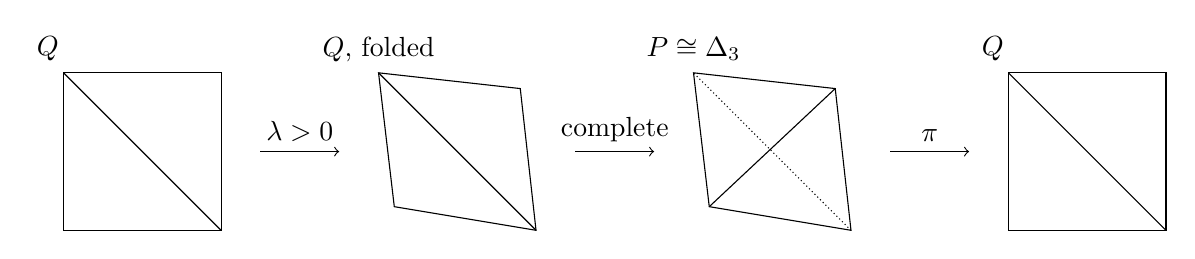
\begin{tikzpicture}[scale=1]
\coordinate (A) at (0,0);
\coordinate (B) at (2,0);
\coordinate (C) at (2,2);
\coordinate (D) at (0,2);

\draw (A) -- (B) -- (C) -- (D) -- cycle;
\draw (B) -- (D);
\node[xshift = -2mm, yshift = 3mm] at (D) {$Q$};

\draw[->] (2.5,1) -- (3.5,1) node[midway,above] {$\lambda > 0$};

\coordinate (A) at (4.2,.3);
\coordinate (B) at (6,0);
\coordinate (C) at (5.8,1.8);
\coordinate (D) at (4,2);

\draw (A) -- (B) -- (C) -- (D) -- cycle;
\draw (B) -- (D);
\node[xshift = 0mm, yshift = 3mm] at (D) {$Q$, folded};

\draw[->] (6.5,1) -- (7.5,1) node[midway,above] {complete};

\coordinate (A) at (8.2,.3);
\coordinate (B) at (10,0);
\coordinate (C) at (9.8,1.8);
\coordinate (D) at (8,2);

\draw (A) -- (B) -- (C) -- (D) -- cycle;
\draw[densely dotted] (B) -- (D);
\draw (A) -- (C);
\node[xshift = 0mm, yshift = 3mm] at (D) {$P \cong \Delta_3$};

\draw[->] (10.5,1) -- (11.5,1) node[midway,above] {$\pi$};

\coordinate (A) at (12,0);
\coordinate (B) at (14,0);
\coordinate (C) at (14,2);
\coordinate (D) at (12,2);

\draw (A) -- (B) -- (C) -- (D) -- cycle;
\draw (B) -- (D);
\node[xshift = -2mm, yshift = 3mm] at (D) {$Q$};
\end{tikzpicture}

\caption{Constructing $P$ from $Q$}
\end{figure}
\end{proof}

\item Show that the following $3$-polytope (the \emph{capped prism}) has a nonregular triangulation without new vertices. (Kleinschmidt and Lee, see Lee [357, Sect.\ 6])

\begin{solution}
    We have the following triangulation

\begin{figure}[h]
    \centering
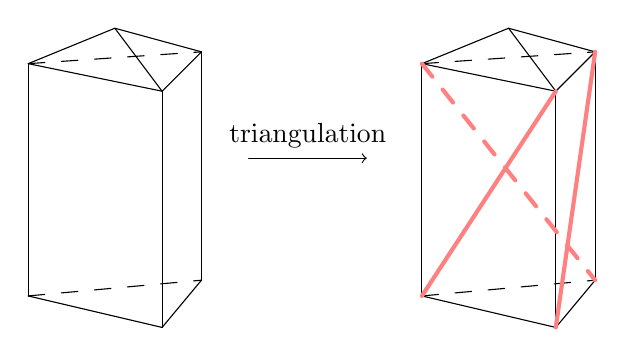
\begin{tikzpicture}[line join=round,line cap=round,scale=1]
\tikzstyle{new edge} = [draw,line width=1.5pt,-,red!50]

\coordinate (A)  at (0,4.2);   
\coordinate (B)  at (1.1,4.65); 
\coordinate (C)  at (2.2,4.35); 
\coordinate (D)  at (1.7,3.85); 

\coordinate (A1) at (0,1.25);   
\coordinate (C1) at (2.2,1.45); 
\coordinate (D1) at (1.7,0.85); 

\draw (A) -- (D) -- (C) -- (B) -- (A);
\draw (A) -- (A1);
\draw (D) -- (D1);
\draw (C) -- (C1);
\draw (A1) -- (D1) -- (C1);
\draw (B) -- (D); 

\draw[dash pattern=on 6pt off 6pt] (A) -- (C);   
\draw[dash pattern=on 6pt off 6pt] (A1) -- (C1); 

\draw[->] (2.8,3) -- (4.3,3) node[midway,above] {triangulation};

\coordinate (A)  at (5,4.2);   
\coordinate (B)  at (6.1,4.65); 
\coordinate (C)  at (7.2,4.35); 
\coordinate (D)  at (6.7,3.85); 

\coordinate (A1) at (5,1.25);   
\coordinate (C1) at (7.2,1.45); 
\coordinate (D1) at (6.7,0.85); 

\draw (A) -- (D) -- (C) -- (B) -- (A);
\draw (A) -- (A1);
\draw (D) -- (D1);
\draw (C) -- (C1);
\draw (A1) -- (D1) -- (C1);
\draw (B) -- (D); 

\draw[dash pattern=on 6pt off 6pt] (A) -- (C);   
\draw[dash pattern=on 6pt off 6pt] (A1) -- (C1); 
\draw[new edge, dash pattern=on 6pt off 6pt] (A) -- (C1);
\draw[new edge] (C) -- (D1);
\draw[new edge] (D) -- (A1);

\end{tikzpicture}
\end{figure}

Lee remarks that "joining the boundary faces to a new point $1$ results in a triangulated 3-sphere that is dual to the Brückner sphere, which is not polytopal".

Alternatively, consider the 3 vertices in the bottom triangle face labeled $1,2,3$. WLOG (by an affine transformation, say) we can fix the coordinates of the top tetrahedron and also fix the direction and length of the 3 vertical edges connecting the top tetrahedron to the bottom triangle. Then the first $3$ coordinates of $[3]$ must be fixed, and write $f(i)$ as the 4th coordinate (i.e. component in $x_4$) of vertex $i$. But then (similar to Ziegler's 2D example, given earlier in the chapter) we get $f(1) > f(2) > f(3) > f(1)$, a contradiction. 
\end{solution}

\item Let $C$ be any polytopal subdivision of a $d$-polytope in $\mathbb{R}^d$.

\begin{enumerate}[label=(\roman*)]
\item Show that the decision of whether $C$ is regular can be reduced to a linear programming feasibility problem. How do you get rid of the strict inequalities that come up?

\item If $C$ is a Schlegel diagram, show that it can be obtained from a ``lower faces'' construction as in Definition 5.3. (Use a projective transformation that moves $\bi{y}_F$ ``to infinity''; compare to Exercise 2.18.)

\item If $C$ is a $d$-diagram, show that the question of whether it is a Schlegel diagram can also be reduced to a linear programming feasibility problem.
\end{enumerate}

\begin{solution}
\begin{enumerate}[label=(\roman*)]
    \item A linear programming feasibility problem asks whether one can find a feasible point that satisfies a collection of linear constraints. Here, the linear constraints are the faces of the $d$-polytope, which all must be lifted as the lower faces of some $d+1$-polytope $P$ so that $\pi(P) = C$ (as per Definition 5.3). We are essentially choosing the $x_{d+1}$ component of every vertex such that the new $d+1$-polytope $P$ is subject to the constraint of every face. We can write a strict inequality $\bi{ax} < b$ as $\bi{ax} \leq b - \lambda$ for some $\lambda > 0$. Alternatively we can always rescale so $\bi{ax} < b$ becomes $\bi{ax} \leq b-1$.

    \item Just move $\bi{y}_F$ to infinity and the result follows.
    \ermactually{I haven't done 2.18 yet skull}

    \item Similar to earlier (by using part (ii)) we are looking for a valid set of $x_{d+1}$ components for each vertex, which raises the polytope of the $d$-diagram $Q$ to a $d+1$-polytope $P$. The constraints are again the $k$-faces. Additionally here we have to determine a viewpoint $\bi{y}_F$
\end{enumerate}
\end{solution}

\item Produce examples of polytopes that have nonregular triangulations without new vertices.

\begin{enumerate}[label=(\roman*)]
\item The $4$-cube $C_4$ has nonregular triangulations without new vertices. 

(It was an open problem for a long time whether $C_d$ has nonregular triangulations for any $d$. Now De Loera [182] has shown that there are even such triangulations with $24$ maximal simplices, all of which have volume $1/4!$.)

\item The second hypersimplices $\Delta_{d-1}(2)$ have nonregular triangulations without new vertices, for $d\ge 9$. (These were constructed, with combinatorial tools by De Loera, Sturmfels \& Thomas [183]; you are allowed to use the computer, via part (i) of the previous exercise. This might in particular be useful in the next two parts, which are unsolved problems.)

\item Can products $\Delta_{m-1}\times\Delta_{n-1}$ of two simplices have nonregular triangulations? (Answer: $\Delta_3\times\Delta_3$ is the product to look at -- De Loera [182].)

\item* Consider the triangulations of the square $[0,n]^2$ with vertex set $\{0,1,\ldots,n\}\times\{0,1,\ldots,n\}$. Estimate the numbers $f(n)$ and $f_{\mathrm{reg}}(n)$ of all triangulations resp.\ of all regular triangulations, as precisely as possible. (Compare your results to those in [298].) Is it true that ``most of'' the triangulations are nonregular, when $n$ gets large, that is, that the ratio $f_{\mathrm{reg}}(n)/f(n)$ tends to $0$ for $n\to\infty$?
\end{enumerate}

\begin{solution}
\begin{enumerate}[label=(\roman*)]
    \item Similar to the previous trick, we use a simplex $\Delta_4$ in the triangulation to "lock down" the coordinates, and then triangulate the rest of the facets to form a sort of "twisted" structure that cannot occur in dimension one higher. Or, written explicitly, a chain of inequalities $f(1) > f(2) > \ldots > f(k) > f(1)$, which is a contradiction. 
    
\begin{figure}[h]
 \centering
 \scalebox{0.8}
 {
 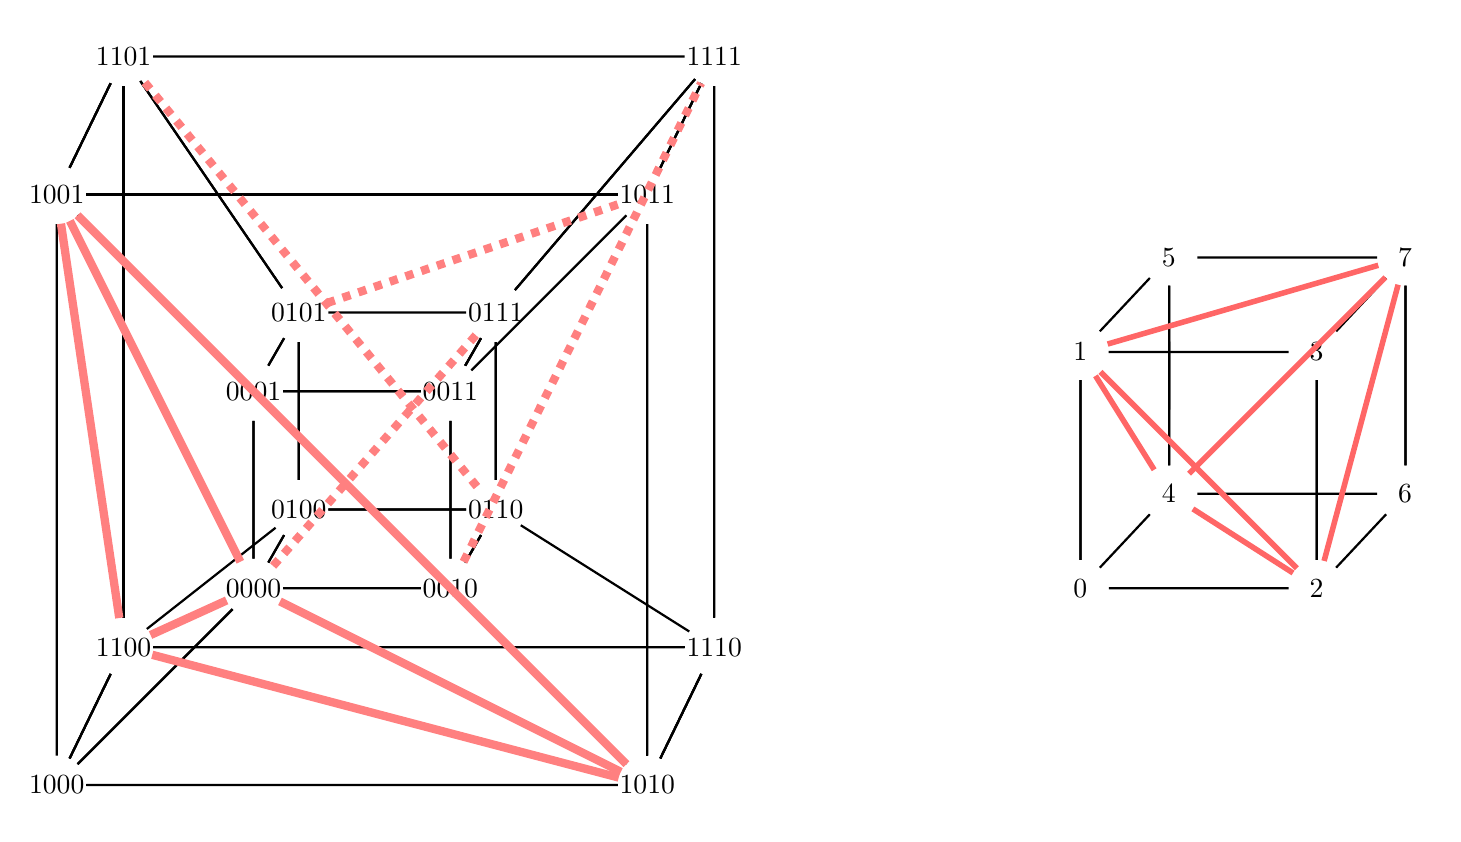
\begin{tikzpicture}[scale=2.5]
	 \tikzstyle{vertex}=[circle,minimum size=20pt,inner sep=0pt]
	 \tikzstyle{selected vertex} = [vertex, fill=red!24]
  \tikzstyle{new edge} = [draw,line width=3pt,-,red!50]
  \tikzstyle{bruh} = [draw,line width=2pt,-,red!60]
	 \tikzstyle{edge} = [draw,thick,-,black]

	 \node[vertex] (v0) at (0,0) {$0000$};
	 \node[vertex] (v1) at (0,1) {$0001$};
	 \node[vertex] (v2) at (1,0) {$0010$};
	 \node[vertex] (v3) at (1,1) {$0011$};
	 \node[vertex] (v4) at (0.23, 0.4) {$0100$};
	 \node[vertex] (v5) at (0.23,1.4) {$0101$};
	 \node[vertex] (v6) at (1.23,0.4) {$0110$};
	 \node[vertex] (v7) at (1.23,1.4) {$0111$};
	 \node[vertex] (v8) at (-1,-1) {$1000$};
	 \node[vertex] (v9) at (-1,2) {$1001$};
	 \node[vertex] (v13) at (-0.66,2.7) {$1101$};
	 \node[vertex] (v12) at (-0.66,-0.3) {$1100$};
	 \node[vertex] (v10) at (2,-1) {$1010$};
	 \node[vertex] (v14) at (2.34,-0.3) {$1110$};
	 \node[vertex] (v11) at (2,2) {$1011$};
	 \node[vertex] (v15) at (2.34,2.7) {$1111$};

	 \draw[edge] (v0) -- (v1) -- (v3) -- (v2) -- (v0);
	 \draw[edge] (v0) -- (v4) -- (v5) -- (v1) -- (v0);
	 \draw[edge] (v2) -- (v6) -- (v7) -- (v3) -- (v2);
	 \draw[edge] (v4) -- (v6) -- (v7) -- (v5) -- (v4);
	 \draw[edge] (v8) -- (v9) -- (v13) -- (v12) -- (v8);
	 \draw[edge] (v0) -- (v4) -- (v12) -- (v8) -- (v0);
	 \draw[edge] (v1) -- (v9) -- (v13) -- (v5) -- (v1);
	 \draw[edge] (v2) -- (v10) -- (v14) -- (v6) -- (v2);
	 \draw[edge] (v8) -- (v10) -- (v14) -- (v12) -- (v8);
	 \draw[edge] (v3) -- (v11) -- (v15) -- (v7) -- (v3);
	 \draw[edge] (v10) -- (v11) -- (v15) -- (v14) -- (v10);
	 \draw[edge] (v9) -- (v11) -- (v15) -- (v13) -- (v9);
	 \draw[edge] (v0) -- (v2);
	 \draw[edge] (v2) -- (v6);
	 \draw[edge] (v6) -- (v4);
	 \draw[edge] (v4) -- (v5);
	 \draw[edge] (v5) -- (v13);
	 \draw[edge] (v13) -- (v12);
	 \draw[edge] (v12) -- (v14);
	 \draw[edge] (v14) -- (v15);
	 \draw[edge] (v15) -- (v7);
	 \draw[edge] (v7) -- (v3);
	 \draw[edge] (v3) -- (v1);
	 \draw[edge] (v1) -- (v9);
	 \draw[edge] (v9) -- (v11);
	 \draw[edge] (v11) -- (v10);
	 \draw[edge] (v10) -- (v8);
	 \draw[edge] (v8) -- (v0);
  \draw[new edge] (v0) -- (v9);
  \draw[new edge] (v0) -- (v10);
  \draw[new edge] (v0) -- (v12);
  \draw[new edge] (v9) -- (v10);
  \draw[new edge] (v9) -- (v12);
  \draw[new edge] (v10) -- (v12);
  \draw[new edge, dashed] (v2) -- (v15);
  \draw[new edge, dashed] (v5) -- (v11);
  \draw[new edge, dashed] (v6) -- (v13);
  \draw[new edge, dashed] (v0) -- (v7);

  \node[vertex] (v0) at (4.2,0) {0};
	 \node[vertex] (v1) at (4.2,1.2) {1};
	 \node[vertex] (v2) at (5.4,0) {2};
	 \node[vertex] (v3) at (5.4,1.2) {3};
	 \node[vertex] (v4) at (4.65, 0.48) {4};
	 \node[vertex] (v5) at (4.65,1.68) {5};
	 \node[vertex] (v6) at (5.85,0.48) {6};
	 \node[vertex] (v7) at (5.85,1.68) {7};
  \draw[edge] (v0) -- (v1) -- (v3) -- (v2) -- (v0);
	 \draw[edge] (v0) -- (v4) -- (v5) -- (v1) -- (v0);
	 \draw[edge] (v2) -- (v6) -- (v7) -- (v3) -- (v2);
	 \draw[edge] (v4) -- (v6) -- (v7) -- (v5) -- (v4);
  \draw[bruh] (v1) -- (v4);
  \draw[bruh] (v4) -- (v2);
  \draw[bruh] (v1) -- (v7);
  \draw[bruh] (v7) -- (v4);
  \draw[bruh] (v7) -- (v2);
  \draw[bruh] (v1) -- (v2);
  
  
 \end{tikzpicture}
 }
 \caption{Non-regular triangulation of $C_4$, and the (sub)triangulation of $C_3$}
 \end{figure}

In this $C_4$ we have the vertices $0000, 1000, 1001, 1010, 1100$ as the vertices for the $4$-simplex. Then, the remaining $4$ facets ($C_3$) are triangulated as per the $C_3$ (sub)triangulation, oriented to agree with the dotted edges.

\item Ok.

\item Just read [182]

\item I uhm, I don't know really
\end{enumerate}
\end{solution}

\item Define the product of two polyhedral complexes, in such a way that the product of subdivisions of two polytopes $P$ and $Q$ is a subdivision of the product $P\times Q$. Prove that the product subdivision is regular if and only if the original subdivisions of $P$ and $Q$ were regular.

\begin{solution}
    Denote $\mathcal{C}(P)$ as a subdivision with underlying set $P$. We want $\mathcal{C}(P) \times \mathcal{C}(Q) = \mathcal{C}(P\times Q)$. We have a natural bijection $\operatorname{vert}(P) \times \operatorname{vert}(Q) \cong \operatorname{vert}(P\times Q)$. In this way, we want a $k$-face $S \cong S_P \times S_Q \in \mathcal{C}(P) \times \mathcal{C}(Q)$ if and only if $S_P$ is a face in $S$ and $S_Q$ is a face in $Q$. In other words, define
    \[\mathcal{C}(P) \times \mathcal{C}(Q) := \{F \times G: F \in \mathcal{C}(P), Q\in \mathcal{C}(Q)\}.\]
    and it is clear that $\mathcal{C}(P) \times \mathcal{C}(Q)$ is a subdivision of the product $P\times Q$. Also note that for the trivial subdivision $\mathcal{C}(P) = P$ we recover the definition of the polytope (Cartesian) product.

    Now assume that $\mathcal{C}(P), \mathcal{C}(Q)$ are regular, then  \ermactually{mi bombo}
\end{solution}

\item Compute the numbers $f_k$ of $k$-faces for the polytope $\widetilde{\mathcal{P}}_4(z_1,z_2,z_3)$.

\begin{solution}
    We have
    \[\vec{f}(\widetilde{\mathcal{P}}_4(z_1,z_2,z_3)) = \begin{pmatrix}
        f_{-1} \\ f_0 \\ f_1 \\ f_2 \\ f_3 \\ f_4
    \end{pmatrix} = \begin{pmatrix}
        1 \\ (z_1+1)(z_2+1)(z_3+1) \\ 12+ z_1(z_2+1)(z_3+1)+z_2(z_1+1)(z_3+1)+z_3(z_1+1)(z_2+1) \\ 18+2(z_1z_2+z_2z_3+z_3z_1) + z_1z_2(z_3-1)+z_2z_3(z_1-1)+ z_3z_1(z_2-1) \\ 7+z_1z_2z_3 \\ 1
    \end{pmatrix}\]

We can see this by noticing that $\widetilde{\mathcal{P}}_4(z_1,z_2,z_3)$ is essentially a $C_3$ cube containing the pile of cubes $\mathcal{P}_3(z_1,z_2,z_3)$, sharing the same vertices. Thus $f_0$ is just the vertex count of the pile of cubes. For $f_1$ we add the $12$ edges in $C_3$ to the edges in $\mathcal{P}_3$. For $f_2$ we have $6$ $2$-faces from $C_3$, $12$ $2$-faces created between an edge of $C_3$ and the corresponding side of $\mathcal{P}_3$, and the $2$-faces of $\mathcal{P}_3$. For its facets we have $C_3$ as 1, then 6 more formed by a face of the cube with the corresponding face of $\mathcal{P}_3$, and the number of cubes in $\mathcal{P}_3$.

One can also check that $\vec{f}(\widetilde{\mathcal{P}}_4(z_1,z_2,z_3))$ satisfies the Euler-Poincare formula, which says that $\sum_{i=-1}^n (-1)^if_i = 1-(-1)^n$.
\end{solution}

\item A ``default'' convex function is given by the paraboloid function
\[
f:\mathbb{R}^d\to\mathbb{R},\quad \bi{x}\mapsto \sum_{i=1}^d x_i^2.
\]
Let $V\subseteq \mathbb{R}^d$ be a finite set of points (vertices). Show that the regular subdivision of $Q:=\mathrm{conv}(V)$ associated with this $f$ has the following property: for every facet of the subdivision there is a sphere that contains all its vertices, but no other vertices from $V$. 

(This subdivision is known as the \emph{Delaunay triangulation} of the point set $V$. It is of great importance for many aspects of computational geometry; see for example Edelsbrunner [190].)

\begin{proof}
    For $\bi{v} \in V$ write $\bi{v}' = \begin{pmatrix}
        \bi{v} \\ ||\bi{v}||^2
    \end{pmatrix}\in \mathbb{R}^{d+1}$. 

    \ermactually{genuinely cooked vro}
\end{proof}


\item Show that the following $2$-diagram is regular, but not Schlegel:

\begin{figure}[h]
    \centering
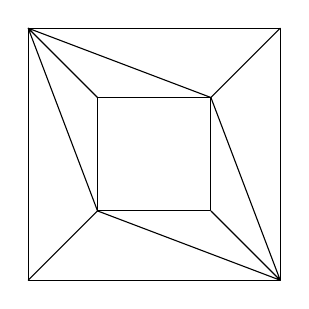
\begin{tikzpicture}[scale=0.8, line join=round, line cap=round]
  \coordinate (A) at (0,4);
  \coordinate (B) at (4,4);
  \coordinate (C) at (4,0);
  \coordinate (D) at (0,0);

  \coordinate (E) at (1.1,2.9);
  \coordinate (F) at (2.9,2.9);
  \coordinate (G) at (2.9,1.1);
  \coordinate (H) at (1.1,1.1);

  \draw (A)--(B)--(C)--(D)--cycle;
  \draw (E)--(F)--(G)--(H)--cycle;

  \draw (A)--(E) (A)--(F) (A)--(H);
  \draw (B)--(F);
  \draw (C)--(F) (C)--(G) (C)--(H);
  \draw (D)--(H);
\end{tikzpicture}
\end{figure}

\begin{solution}
    Regularity can be easily seen by a direct construction. Assume by contradiction we have some 3-polytope $P$ and a facet $F$ for which the Schlegel diagram $\mathcal{D}(P, F)$ is (exactly, not just combinatorially equivalent to) the above 2-diagram. Then, clearly all of the triangulated trapezoids (in the 2-diagram) must have have its $4$ vertices non-coplanar, or else the triangulating diagonal edge is not an edge in $P$. Label the 4 vertices of the outer square as $[4]$. The inner square is planar so the edge between neighboring vertices in the outer square must not be parallel to the corresponding edge in the inner square, and so the $x_3$ components of vertices $[4]$ cannot all be the same.. But then there must be more edges than shown in the diagram (edge $(1,3)$ or $(2,4)$), contradiction.

    Note that although every Schlegel diagram is regular, this counterexample disproves the converse, in general. Furthermore, it is the case that every 2-diagram is \textit{combinatorially equivalent} to a Schlegel diagram, as per Theorem 5.8.
\end{solution}

\item Show that in general the polytopal complex $\mathcal C(\partial P)\setminus\{F\}$ and the Schlegel diagram $\mathcal D(P,F)$ are not affinely isomorphic. (For this, it suffices to consider the $3$-cube!) 

However, show that $p: G\to p(G)$ is a projective transformation, for all proper faces $G$ of $P$.

\begin{proof}
    Consider the 3-cube $C_3$. For a facet $F$ (they're all the same up to symmetry) we have the following Schlegel diagram, which is clearly not affinely isomorphic to the edges of $C_3$ by parallelism.

    However, every $p: G \to p(G)$ for a proper face $G \subseteq P$ is a projective transformation; from the viewpoint $\bi{y}_F$ one is essentially coning the face $G$ and then slicing it by the chosen facet $F$, as per Chapter 2.6.
\begin{figure}[h]
    \centering
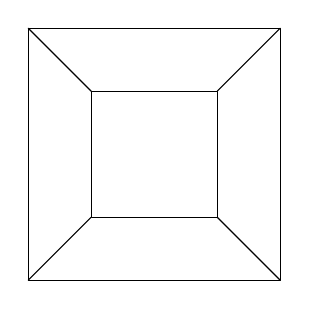
\begin{tikzpicture}[scale=0.8, line join=round, line cap=round]
  \coordinate (A) at (0,4);
  \coordinate (B) at (4,4);
  \coordinate (C) at (4,0);
  \coordinate (D) at (0,0);

  \coordinate (E) at (1,3);
  \coordinate (F) at (3,3);
  \coordinate (G) at (3,1);
  \coordinate (H) at (1,1);

  \draw (A)--(B)--(C)--(D)--cycle;
  \draw (E)--(F)--(G)--(H)--cycle;

  \draw (A)--(E);
  \draw (B)--(F);
  \draw (C)--(G);
  \draw (D)--(H);
\end{tikzpicture}

\caption{Schlegel diagram of $C_3$}
\end{figure}
\end{proof}

\item Construct a Schlegel diagram for the polar of a product
\[P=(\Delta_2 \times \Delta_2)^{\Delta}.\]

Construct Schlegel diagrams for the cyclic polytopes $C_3(6)$ and $C_4(7)$.

\begin{solution}
    Recall by Exercise 0.6 we have that $(\Delta_2 \times \Delta_2)^{\Delta} \cong C_4(6)$, which is easier to work with. By Gale's evenness condition we know $C_4(6)$ has a facet $F = 1234$, where we can pick a point $\bi{y}_F$ beyond $F$ as $\frac{\sum_{i=1}^4 \textbf{x}(i)}{4} - \lambda$ for $\lambda > \textbf{0}$. For the sake of computation, pick $\lambda = 0.1\cdot\textbf{1}$, so $\bi{y}_F = (2.4, 7.4, 24.9, 88.4)$ Explicitly write the equation for $F$ as $50x_1-35x_2+10x_3-x_4=24$. Then the line from $\textbf{x}(5)$ to $\bi{y}_F$ intersects $F$ at point $(\frac{19}{9}, \frac{49}{9}, \frac{124}{9},\frac{259}{9})$. Similarly, $\textbf{x}(6)$ intersects $F$ at point $(\frac{114}{49},\frac{334}{49},21,\frac{3124}{49})$. Now use an affine transformation to send $F$ to $\mathbb{R}^3$ and we can draw the Schlegel diagram.

    $C_4(7)$ is the same story as $C_4(6)$. In fact, the point of intersection for $\textbf{x}(7)$ is $(\frac{353}{149},\frac{1061}{149},\frac{3392}{149},\frac{10859}{149})$. We will leave the rest. 

    The Schlegel diagram of $C_3(6)$ is 2 dimensional so we will draw it. We use the facet $F = 123$ and perform a similar procedure:

\begin{figure}[h]
    \centering
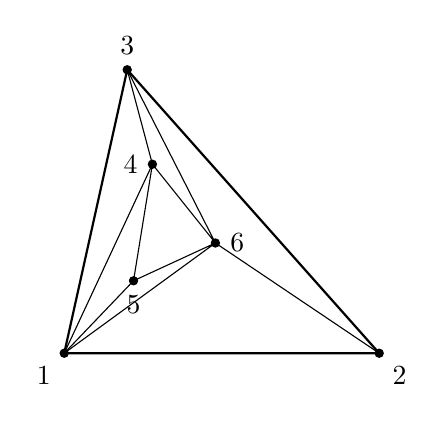
\begin{tikzpicture}[scale=4, line join=round, line cap=round,
  v/.style={circle, fill=black, inner sep=1.2pt},
  lab/.style={font=\small}
]
  \coordinate (1) at (0.00,0.00);
  \coordinate (2) at (1.00,0.00);
  \coordinate (3) at (0.20,0.90);

  \coordinate (6) at (0.48,0.35);
  \coordinate (4) at (0.28,0.60);
  \coordinate (5) at (0.22,0.23);
  
  \draw[thick] (1)--(2)--(3)--cycle;

  \draw (1)--(4) (3)--(4);
  \draw (1)--(5) (4)--(5);
  \draw (1)--(6) (2)--(6) (3)--(6) (4)--(6) (5)--(6);

  \node[v,label=below left:{$1$}] at (1) {};
  \node[v,label=below right:{$2$}] at (2) {};
  \node[v,label=above:{$3$}] at (3) {};
  \node[v,label=left:{$4$}] at (4) {};
  \node[v,label=below:{$5$}] at (5) {};
  \node[v,label=right:{$6$}] at (6) {};
\end{tikzpicture}
\caption{Schlegel diagram of $C_3(6)$}
\end{figure}

One can use Gale's evenness condition to verify edge connectivity for themselves.
\end{solution}

\item* What is the smallest number $f(d)$ of $d$-simplices that is sufficient to triangulate a $d$-cube?

Combining results by Hughes and Anderson [285] [287] [286] [288] and Haiman [267], we know that
\[f(2)=2,\; f(3)=5,\; f(4)=16,\; f(5)=67,\; f(6)=308,\; f(7)=1493,\; \text{and}\; 5522 \le f(8) \le 11944.\]
For large $d$ a method due to Smith [505], using volume estimates in hyperbolic geometry, yields the best lower bounds on $f(d)$ so far.

Is it true that the smallest number is always/only achieved by a triangulation without new vertices?

What is the maximal number of simplices that may be needed to triangulate any $0/1$-polytope? Is this the same number you get in case of the $d$-cube?

(``Efficient'' triangulations of $d$-cubes, with few facets, have been studied extensively, for example for use in finite element methods for solving differential equations. Thus, a lot is known about such triangulations. For example, one knows that asymptotically, at most $\rho^d d!$ simplices are needed for large $d$, for some constant $\rho<1$. We refer to Haiman [267] and Todd \& Tun\c{c}el [545] for more information.)

\item For a $4$-polytope, one cannot prescribe the shape of a $2$-face! Namely, Richter-Gebert [459, p.~91] [462] provides the following diagram of a $4$-dimensional polytope $X^*$:
\begin{figure}[h]
    \centering
    \includegraphics[width=0.3\linewidth]{images/Ziegler 5.11.png}
\end{figure}

Show that this represents the Schlegel diagram of a $4$-polytope with $8$ facets and $12$ vertices. Show that the shape of the hexagon at the base cannot be prescribed arbitrarily: three lines, determined by two opposite edges and by the diagonal between them, must (projectively) meet in a point. (See also Exercise 6.11)

\begin{solution}
    The fact that the three lines need to meet at a point, even projectively, means a constriant on the shape of the hexagon which a general hexagon will fail to satisfy. See Exercise 6.11

\begin{remark}
    
    To be clear, the three lines refers to the following lines, which meet at the same point projectively in this case.

\begin{figure}[h]
    \centering
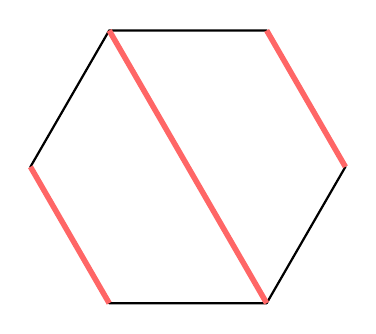
\begin{tikzpicture}[scale=2, line join=round]
\tikzstyle{bruh} = [draw,line width=2pt,-,red!60]
  \foreach \i/\ang in {1/0,2/60,3/120,4/180,5/240,6/300}{
    \coordinate (v\i) at (\ang:1);
  }
  \draw[thick] (v1)--(v2)--(v3)--(v4)--(v5)--(v6)--cycle;
  \draw[bruh] (v3) -- (v6);
  \draw[bruh] (v1) -- (v2);
  \draw[bruh] (v4) -- (v5);
\end{tikzpicture}

\caption{The Hexagon 2-Face of Richter-Gebert's 4-Polytope}
\end{figure}
\end{remark}
\end{solution}

\item Show that $2^d$ simplices can be arranged in $\mathbb{R}^d$ in such a way that any two are adjacent (that is, the intersections are $(d-1)$-dimensional).

\begin{remark}
    Here $(d-1)$-dimensional does not mean a proper facet for both adjacent polytopes (i.e. we don't need $P \cap P' = F \in L(P), L(P')$). It just means "a patch of $\mathbb{R}^{d-1}$", essentially. See the $d=2$ illustration below.
\end{remark}

\begin{figure}[h]
    \centering
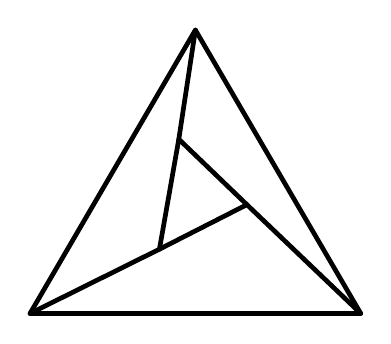
\begin{tikzpicture}[scale=0.6, line cap=round,line join=round]
  \coordinate (A) at (0,0);
  \coordinate (B) at (7,0);
  \coordinate (C) at (3.5,6);

  \coordinate (P) at (2.739,1.361);
  \coordinate (Q) at (3.149,3.689);
  \coordinate (T) at (4.590,2.304);

  \draw[line width=1.7pt] (A)--(B)--(C)--(A);

  \draw[line width=1.7pt] (C)--(Q)--(P);
  \draw[line width=1.7pt] (A)--(P)--(T);
  \draw[line width=1.7pt] (Q)--(T)--(B);
\end{tikzpicture}

    \caption{$d=2$}
\end{figure}

\begin{proof}
\ermactually{this one is really cool i think im gonna come back to it!!}    
\end{proof}


\item The smallest triangulation of the torus surface has $7$ vertices, $21$ edges and $14$ triangles. Construct it, and show that it can be embedded as a subcomplex into $\mathcal C(C_4(7))$, and thus as a simplicial complex into $\mathbb{R}^3$.
(Cs\'asz\'ar [169], Gr\"unbaum [252, p.~253]; see also Altshuler [14] and Bokowski \& Eggert [113])

\begin{remark}
    Ziegler writes $C_7(4)$ mistakenly, we believe. It has been corrected to $C_4(7)$ here.
\end{remark}

\begin{solution}
    We are embedding $K_7$ on a torus, essentially. It is lesser known that a torus can be represented as folding up a hexagon (pick a pair of opposite edges and glue them together, then twist the tube and connect the ends. Note that in the remaining 4 pairs of edges, it is not the opposite pairs of edges that are glued together. Instead, co-identified pairs are symmetric about the line through the center of the hexagon perpendicular to both of the edges glued together initially. More concretely, label edges $[6]$ cyclically, and glue $3-6$. Then we have $1-5$ and $2-4$.). We have

\begin{figure}[h]
    \centering
    \includegraphics[width=0.4\linewidth]{images/K7 on a torus.png}
    \caption{Minimal Triangulation of a Torus}
\end{figure}


Recall that $C_d(n)$ is $\lfloor \frac{d}{2} \rfloor$-neighborly, so indeed it can be embedded as a subcomplex of $\mathcal{C}(C_4(7))$. The simplicial complex embedding in $\mathbb{R}^3$ follows from Exercise 5.9 (i.e. the Schlegel diagram of $C_4(7)$) and Exercise 0.10 (that every $2\lfloor \frac{d}{2} \rfloor - 1 = 3$-face is a simplex, hence simplicial complex).
\end{solution}

\item* Can \emph{every} triangulation of the torus be realized by a simplicial complex $C$ in $\mathbb{R}^3$?

(This is a classical problem of Gr\"unbaum [252, p.~253], which is still wide open. See Ewald, Kleinschmidt, Pachner \& Schulz [203, p.~153],qq Altshuler, Bokowski \& Schuchert [15] and their references.)

\item Show that every $d$-dimensional simplicial complex can be realized as a subcomplex of a simplicial $(2d+2)$-polytope, and thus has a straight realization as a simplicial complex in $\mathbb{R}^{2d+1}$.

(Hint: Take a suitable cyclic polytope and its Schlegel diagram.)

\begin{solution}
    Let the simplicial complex $\mathcal{K}$ have $n$ vertices. Then we can embed it in $\mathcal{C}(C_{2d+2}(\max\{2d+3, n\}))$ because it is $d+1$-neighborly. Taking the Schlegel diagram of the cyclic polytope, we obtain the straight realization in $\mathbb{R}^{2d+1}$ 
\end{solution}

\item Show that there are polyhedral complexes that are not subcomplexes of polytopes. Namely, show that the subdivision of the \emph{M\"obius band} drawn below with $6$ vertices, $10$ edges, and $4$ facets can be realized as a polyhedral complex in $\mathbb{R}^3$, but not as a subcomplex of any polytope. (figure omitted)

(This is due to Betke, Schulz \& Wills [68]; see Barnette [48] for a similar, but simplicial, M\"obius strip that serves as an ``impediment for polyhedrality.'' It is not even true that every triangulated M\"obius strip has a straight embedding into $\mathbb{R}^3$: see Brehm [129]. However, the Schlegel diagram construction shows that no such M\"obius strip can appear in the boundary of a $4$-polytope.)

\begin{solution}
    Indeed it is a polyhedral complex (just check Definition 5.1), and because it "folds over itself" in a non-convex way it cannot be a subcomplex of any polytope; one of the faces of the Möbius band will not be a face of the polytope.
\end{solution}

\item Modify Schulz' $3$-diagram $D_1$ from Example 5.10 by subdividing the bipyramid $A$ into three tetrahedra, $[2,3,6]$, $[2,5,6]$, and $[2,6,7]$. Show that this yields a new $3$-diagram $D_1'$ with $8$ vertices and $12$ facets, which contains the M\"obius band of the previous exercise as a subcomplex. 

Derive that $D_1'$ is not polytopal, either.

\begin{solution}
    Immediate.
    \ermactually{stop the cap}
\end{solution}
\end{enumerate}

\bigskip
\section{Duality, Gale Diagrams, and Applications}

\begin{enumerate}
\setcounter{enumi}{-1}
\renewcommand{\labelenumi}{6.\arabic{enumi}}
\item Prove \emph{Radon}'s theorem: given any set $V$ of $d+2$ points in $\mathbb{R}^d$, we can find disjoint nonempty subsets $V_1,V_2\subseteq V$ such that $\operatorname{relint}(\operatorname{conv}(V_1))\cap \operatorname{relint}(\operatorname{conv}(V_2))\neq \varnothing$. Why can we assume that $\operatorname{conv}(V_i)$ are simplices?

\begin{proof}
    Write $V = (v_1, \ldots, v_{d+2})$. Recall that $\conv(V) = \{V\bi{x}: \bi{x} \geq \textbf{0}, \mathds{1}\bi{x} = 1\}$. Notice we have $\rank \begin{pmatrix}
        \textbf{1} \\ V
    \end{pmatrix} \leq d+1$. Thus there exists $\bi{x} \in \mathbb{R}^{d+2}$ such that $\begin{pmatrix}
        \textbf{1} \\ V
    \end{pmatrix}\bi{x} = \textbf{0}$. Split $\bi{x} = \bi{x}^+ - \bi{x}^-$ with $\bi{x}^+, \bi{x}^- \geq 0$ and we obtain the desired partition: $V_1$ corresponding to the non-zero components of $\bi{x}^+$ and $V_2$ to $\bi{x}^-$. We can assume $\conv(V_i)$ are simplicies because we can simply exclude the vertices corresponding to entries in $\bi{x}^+, \bi{x}^-$ which equal $0$
\end{proof}

\item Show that if two configurations of $n$ points in $\mathbb{R}^d$ have the same set of minimal affine dependencies, then they are affinely isomorphic.

\begin{proof}
    A vector $\bi{z}$ is an affine dependence (i.e. $\bi{z} \in \aDep(X)$) if and only if it is a (finite) sum of affine minimal dependencies. Thus the matricies $\begin{pmatrix}
        \mathds{1} \\ V
    \end{pmatrix}$ and $\begin{pmatrix}
        \mathds{1} \\ W
    \end{pmatrix}$ have the same row space, so they differ only by a change of coordinates.
    
    Concretely. isomorphism is induced by the sign vectors, where we have (informally) $\MIN(\aDep(V)) = \MIN(\aDep(W)) \implies \SIGN(\aDep(V) / \mathbb{R}) = \SIGN(\aDep(W) / \mathbb{R})$, where we quotient by $\mathbb{R}$ because if $\bi{z}$ is an affine dependency then so is $\lambda\bi{z}$, for all $\lambda \in \mathbb{R}$. One could also normalize like Ziegler does by writing $\Lambda$ as the sum of the positive components (which is equivalent to the negative sum of the negative components) of some dependency $\bi{z}$ and write $y:=\sum_{i\in P(\bi{z})} \frac{z_i}{\Lambda}x_i = \sum_{i\in N(\bi{z})} \frac{-z_i}{\Lambda}x_i $.
\end{proof}

\item List all the circuits and cocircuits for the hexagon discussed in Section~6.1. How many vectors and covectors are there? (Don't list them all, there are many.)

\begin{solution}
    The hexagon has vertex set $X = \begin{pmatrix}
        0 & 3 & 5 & 5 & 2 & 0 \\ 0 & 0 & 1 & 2 & 2 & 1
    \end{pmatrix}$. 
\begin{figure}[h]
    \centering
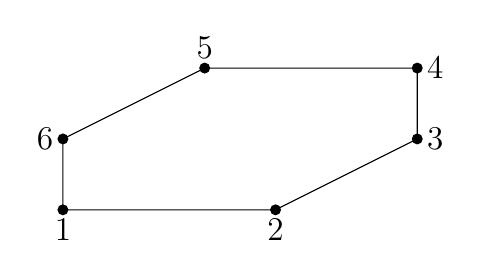
\begin{tikzpicture}[scale=0.9, every node/.style={font=\large}]
  \coordinate (v1) at (0,0);
  \coordinate (v2) at (3,0);
  \coordinate (v3) at (5,1);
  \coordinate (v4) at (5,2);
  \coordinate (v5) at (2,2);
  \coordinate (v6) at (0,1);

  \draw (v1) -- (v2) -- (v3) -- (v4) -- (v5) -- (v6) -- cycle;

  \foreach \i in {1,2,3,4,5,6}{\fill (v\i) circle (2.2pt);}

  \node[below] at (v1) {1};
  \node[below] at (v2) {2};
  \node[right] at (v3) {3};
  \node[right] at (v4) {4};
  \node[above] at (v5) {5};
  \node[left]  at (v6) {6};
\end{tikzpicture}
\caption{$\conv(X)$}
\end{figure}
    
    We will just write the partition of vertices $(V_1, V_2)$ for each circuit. We have the following circuits
    \[(13 ,24), (13, 25), (13, 26), (14, 25), (14, 26), (14, 35), (14, 36), \]
    \[(15, 26), (15, 36), (15, 46), (24, 35), (24, 36), (25, 36), (25, 46), (35, 46).\]
    and the cocircuits are simply the hyperplanes spanned by the vertices $\binom{[6]}{2}$.

    In total, there are $15+39+\frac{1}{2}\binom{6}{3}- 3 = 61$ vectors and $2+\binom{6}{2}+5\cdot 6+\binom{6}{2} = 62$ covectors.
    
\end{solution}

\item Show that the definitions of vectors, circuits, and so on, for the affine and linear cases are consistent: if $V=\begin{pmatrix}
\mathds{1}\\ X 
\end{pmatrix},$then
\[\text{a-Dep}(X)=\text{Dep}(V) \quad\text{and}\quad \text{a-Val}(X)=\text{Val}(V),\]
and thus we get the same oriented matroid (the same circuits, cocircuits, etc.) for $X$ and for $V$.

\begin{proof}
    $\aDep(X) = \{\bi{z}: X\bi{z} = 0, \mathds{1}\bi{z} = 0\} = \{\bi{z}: \begin{pmatrix}
        \mathds{1} \\ X
    \end{pmatrix}\bi{z} = 0\} = \Dep(V)$.
\end{proof}

\item Let $D=(V,A)$ be a directed graph with arc set $A=\{1,2,\dots,n\}$. 

Define the signed circuits of $D$ to be the sign vectors $\textsc{u}\in\{0,+,-\}^n$ that correspond to circuits in $D$ together with a chosen orientation, as follows: if the arc $i$ is not contained in the circuit, then $u_i=0$; if it is in the circuit and directed according to the orientation, then $u_i=+$; and if it is directed opposite to the orientation, then $u_i=-$. For example, for the digraph drawn here and the oriented circuit marked in it we read off the signed circuit \textsc{u} next to the drawing. Show that the signed circuits we get that way are from a realizable oriented matroid (as in Definition 6.5), whose cocircuits correspond to the minimal directed cuts in the graph. Interpret the vectors and the covectors of this oriented matroid in terms of the graph.

(Hint: Associate a vector configuration with $D$. A canonical choice is $\bi{v}_{ij} = \bi{e}_i - \bi{e}_j$ for an arc from the node $i$ to the node $j$).

\begin{solution}
    Label the vertex set $V$ of a digraph $D$ as $[k]$, and associate vector $\bi{e}_i$ with vertex $i$. In this way associate a directed edge from $i$ to $j$ by the vector $\bi{v}_{ij} = \bi{e}_i - \bi{e}_j$, and consider the oriented matroid $\mathcal{M}(V)$ generated this way. It is easy to see that the signed circuits are the circuits of $\mathcal{M}(V)$, and the corcircuits correspond to minimal directed cuts in the graph. Furthermore, the vectors of directed graph $D$ correspond to the symmetric differences of (the edge set of these) circuits of $\mathcal{M}(V)$ (i.e. dependent sets), and the covectors of $D$ correspond to dependent sets in $\mathcal{M}(V)^*$, or simply the directed cuts of the graph.
\end{solution}

\item Prove that our two characterizations of \emph{acyclic} vector configurations are equivalent. Prove that the dual of an acyclic configuration is totally cyclic (Corollary 6.16). Describe a small vector configuration that is neither acyclic nor totally cyclic.

\begin{proof}
First we state the dual of Farkas Lemma I
\begin{proposition}[FL I, dual]

Let $A \in \mathbb{R}^{d\times m}$ and $\bi{z} \in (\mathbb{R}^m)^*$.

\textbf{Either} there exists a point $x \in (\mathbb{R}^d)^*$ with $\bi{x}A \le \bi{z}$,

\textbf{or} there exists a row vector $\bi{c} \in \mathbb{R}^m$ with $\bi{c} \ge \textbf{0}$, $\bi{c}A= \textbf{0}$ and $\bi{zc}<0$, but not both.
\end{proposition}

To prove the equivalency of the two characterizations for acyclic vector configurations, write $\bi{z} = -\lambda \mathds{1}$ for some $\lambda > 0$ consider the following equivalences
\begin{flalign*}
    &\nexists \bi{y} \in \mathbb{R}^n: \bi{y} \geq \textbf{0}, \; V\bi{y} = \textbf{0}, \; \bi{y} \neq 0 &\\
    & \iff \nexists \bi{y}: \bi{y} \geq \textbf{0}, \; V\bi{y} = \textbf{0}, \; \bi{zy} < 0 \\
    &\overset{\textup{FL I*}}{\iff} \exists \bi{c}' \in (\mathbb{R}^r)^*: \bi{c}'V \leq \bi{z} \\
    & \iff \exists \bi{c} = -\bi{c}': \bi{c}V > \mathds{O}
\end{flalign*}

where the last line holds because we can take $\lambda$ to be sufficiently small.

\smallskip
Now we prove that acyclic and totally cyclic are dual. Write $W$ as the dual configuration of $V$ and we have
\[V \textup{ acyclic} \overset{\textup{(ii)}}{\iff} (++\ldots+) \in \SIGN(\mathcal{V}^*(V)) \overset{\perp}{\iff} (++\ldots+) \in \SIGN(\mathcal{V}(W)) \overset{\textup{(ii)}}{\iff} W \textup{ totally cyclic}\]
by using condition (ii) in Corollary 6.16 for both acyclic and totally cyclic.

\smallskip
Consider the following vector configuration which is neither acyclic nor totally cyclic; choose
\[\bi{x} = (0,1,0), \; \bi{y} = (1, 0, 1), \; V = \begin{pmatrix}
    1 & 0 & -1 \\ 0 & 1 & 0
\end{pmatrix}.\]

Notice that we have $\bi{y} \geq \textbf{0}, \; \bi{y} \neq \textbf{0}, \; V\bi{y} = \textbf{0}$. Furthermore, $G = \ker(V) = (1,0,1)$, and $G$ is not acyclic because we have $\bi{x} \geq \textbf{0}, \; \bi{x}\neq \textbf{0}, \; G\bi{x} = \textbf{0} $, meaning configuration $V$ is neither acyclic nor totally cyclic.
\end{proof}

\item A $d$-polytope with $n$ vertices is simplicial if and only if every non-empty coface has at least $n-d$ elements. Derive from this a characterization of the (affine) Gale diagrams that represent simplicial polytopes.

\begin{proof}
    Let $P$ be a simplicial polytope, then every nonempty coface has at least $n-d$ vertices. Thus in the Gale diagram of $P$, if $\textbf{0} \in \relint\conv\{g_i: i \in I\}$ for a nonempty subset of vertices $I \subseteq [n]$, then $|I| \geq n-d$.
\end{proof}

\item Given a Gale diagram, how can one (computationally) enumerate the facets of the corresponding polytope?

\begin{solution}
    A point set in a Gale diagram corresponds to a facet (the point set of the facet is the complement vertices) in the corresponding polytope if and only if the relative interior of the convex hull of the points in the Gale diagram contain the origin.
\end{solution}

\item Show that the following diagrams represent the four different combinatorial types of $4$-polytopes with $6$ vertices. 

\begin{figure}[h]
    \centering
    \includegraphics[width=0.8\linewidth]{images/Ziegler 6.8.png}
\end{figure}

Describe the polytopes. 

How many facets, and how many edges do they have? Which polytopes are simple or simplicial? Which polytope is self-dual? Which is $\operatorname{bipyr}(\Delta_3)$? Which is $C_4(6)$?

\begin{solution}
    Label these diagrams 1 to 4 from left to right. Since $4$ has two gray points, we see that it is $\operatorname{pyr}(\operatorname{pyr}(C_2))$. Since $2$ is the only $2$-neighborly diagram, it must be $C_4(6)$, simplicial. Diagram $1$ has $8$ facets, all of which are $\Delta_3$, and thus it is simplicial. In fact, the only missing edge in $1$ is the edge between the two white vertices, so its graph is $K_6 - e$, and it is $\operatorname{bipyr}(\Delta_3)$, a simple polytope. Diagram $3$ has a $\operatorname{bipyr}(\Delta_2)$ and 6 $\Delta_3$ facets, it corresponds to $\operatorname{pyr}(\operatorname{bipyr}(\Delta_2))$ and also has graph $K_6 - e$. 
\end{solution}

\item Describe all the $4$-polytopes with $7$ vertices. For this, use all the ``visualization tools'' that we have developed so far:

\begin{itemize}
\item Schlegel diagrams
\item Gale diagrams
\item combinatorial descriptions (vertex-facet matrix)
\end{itemize}
and show how the various types of data correspond to each other.

\begin{solution}
See \cite[Section~6.3]{grunbaum2003convexpolytopes}.
\end{solution}

\item* What is the smallest number of vertices for a nonrational $4$-polytopes? (Non-rational $4$-polytopes exist by Richter-Gebert's universality theorem, see the Notes for this chapter. The smallest (explicit) example by Richter-Gebert has $33$ vertices and ?? facets [459, p.\ 80]. The minimal number of vertices and facets is not known.)

\item Analyze the $4$-dimensional polytope $X^{*}$ with $8$ facets and $12$ vertices whose polar is given by the affine Gale diagram
\begin{figure}[h]
    \centering
    \includegraphics[width=0.6\linewidth]{images/Ziegler 6.11.png}
\end{figure}

Show that $X^{*}$ has a hexagon $2$-face whose shape cannot be prescribed. Verify that $X^{*}$ is combinatorially equivalent to the polytope whose Schlegel diagram is given by Exercise 5.11.

\begin{solution}
The hexagon 2-face in $X^*$ corresponds to the $2$-coface in the polar affine Gale diagram $G$, which is the pair of overlapping points (1 black, 1 white) at the meet of three lines. It is indeed a face because the other $6$ vertices in $G$ contain $\textbf{0}$ in the relative interior of their convex hull. The three lines which meet (projectively) at the same point correspond to the three cofaces here, one along each of the three lines that meet at the black \& white point; black white black, white black white, and black white black. This forces the three edges in $X^*$ corresponding to the face in $G$ (corresponding to these three configurations (i.e. the complement) in the Gale diagram) to meet at the same point, which means that the shape of the hexagon cannot be prescribed (cf. Exercise 5.11). Combinatorial equivalence can be checked by simply comparing the faces in the Gale diagram $G$ with the faces of $(X^*)^{\Delta}$.
\end{solution}

\item Draw an arbitrary ``nice'' configuration of black and white points into the plane, and analyze:

\begin{enumerate}[label=(\roman*)]
\item Is this the Gale diagram of a polytope? (If not, add points to get one.)
\item What is its dimension and its number of facets?
\item Is it simple or simplicial? Can you describe its facets?
\item Are there vertices that are not adjacent? Can you compute the graph?
\end{enumerate}

\begin{solution}
We construct the following Gale diagram:

\begin{figure}[h]
    \centering
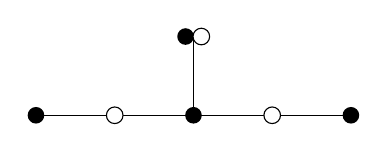
\begin{tikzpicture}[scale=1]
  \draw (-2,0)--(2,0);
  \draw (0,1)--(0,0);
  \fill (-2,0) circle (3pt);
  \fill (0,0)  circle (3pt);
  \fill (2,0)  circle (3pt);
  \fill (-0.1,1)  circle (3pt);

  \draw[fill=white] (-1,0) circle (3pt);
  \draw[fill=white] (1,0)  circle (3pt);
  \draw[fill=white] (.1,1) circle (3pt);
\end{tikzpicture}
\end{figure}

\begin{enumerate}[label=(\roman*)]
    \item Yes
    \item $d=3$, and there are $10$ facets.
    \item Every facet is a triangle, so it is simplicial, but it is not simple.
    \item Yes, the two vertices that are together (one black, one white, overlapping) are not adjacent. In fact, because it is only $d=3$, we can easily identify the polytope: it is $\bipyr(\textup{Pentagon)}$. The five colinear points correspond to the pentagon (try constructing the Gale diagram of the pentagon). 
\end{enumerate}
\end{solution}

\item For $n \ge d \ge 2$, consider the moment curve in $\mathbb{R}^{\,n-d-2}$, and place on it $n$ points, alternating between negative and positive points. Show that the oriented matroid of this is dual to the oriented matroid of the cyclic polytope $C_d(n)$: so it is the Gale diagram of a polytope that is combinatorially equivalent to $C_d(n)$. Is this really a Gale transform of $C_d(n)$?

\begin{proof}
    To show duality of the oriented matroids, it suffices to show that there is a bijection between $\ca{C}(C_{n-d-2})$, the circuits of the (oriented matroid of the) moment curve in $\mathbb{R}^{n-d-2}$, and $\ca{C}^*(C_d(n))$, the cocircuits of the cyclic polytope.
\end{proof}

\item Show that the following conditions are equivalent for a $2d$-dimensional polytope $P$ with $n$ vertices:

\begin{enumerate}[label=(\roman*)]
\item $P$ is neighborly.
\item Every set of $n-d$ points forms the support of a positive covector.
\item Every circuit of $P$ contains exactly $d+1$ positive and $d+1$ negative elements. 
\end{enumerate}

Derive the corresponding criteria to detect whether a Gale diagram represents an (even-dimensional) neighborly polytope.

\begin{remark}
    We have changed the description in (ii) because Ziegler's was unclear, hopefully pointing at the same meaning  (See discussion below Definition 6.2).
\end{remark}

\begin{proof}
We show (i) $\iff$ (ii) and (i) $\iff$ (iii).

Let $P$ be neighborly. Then every set of $d$ vertices is a $(d-1)$-face. Thus every set of $n-d$ points is a coface, which corresponds to the support of a positive covector. Everything was biconditional so the converse follows.

Let $P$ be neighborly. First note that since the circuit is a minimal affine dependency, there can be at most $2d+2$ non-zero components. Now assume by contradiction (WLOG, under a suitable sign change) we get $k$ positive elements, where $k \leq d$. Since $P$ is $d$-neighborly we see that the $k$ positive points form a face $F \subseteq P$, which then means (the affine hull) $\aff(F) \cap \conv(\operatorname{vert}(P) \setminus \operatorname{vert}(F)) = \varnothing$, but which is a contradiction. Conversely suppose every circuit has exactly $d+1$ positive and negative elements. We have the standard lemma that a set $S$ of vertices is a face if and only if there is no circuit whose positive part is contained in $S$. Thus it follows that every vertex set of size at most $d$ corresponds to a face, and thus $P$ is $d$-neighborly.

\smallskip
The corresponding criteria for even-dimensional neighborly Gale diagrams is just that either $\textbf{0} \notin \relint(\conv(S))$ for every set $S$ of $d$ vertices, or that every minimal dependence splits into exactly $d+1$ points on each side. 
\end{proof}

\item Show that of the following two figures, the left is a Gale diagram for $C_4(8)$, while the second is the Gale diagram of a $2$-neighborly $4$-polytope with $8$ vertices that is not cyclic (due to [531, p.\ 543]).

\begin{proof}
By Gale's evenness condition, we obtain the following as facets for $C_4(8)$:
\[1234, 1245, 1256, 1267, 1278, 2378, 3478, 4578, 5678,\]
\[1238, 1348, 1458, 1568, 1678, 2345, 2356, 2367, 3456, 3467, 4567\]

One can explicitly check that the Gale diagram (on the left) produces exactly these facets.

However, in the right hand Gale diagram, we lose facets $1568, 1678, 4567, 4578$, and thus it is not cyclic. Indeed, any $6$ points still contain $\textbf{0}$, so the corresponding polytope is still $2$-neighborly.
\end{proof}

\item* Perles conjectured that every simplicial polytope is combinatorially equivalent to a face figure (iterated vertex figure) of an even-dimensional neighborly polytope. (Equivalently, every simple polytope is a face of a polar of a neighborly polytope.)
\begin{enumerate}[label=(\roman*)]
\item Define that a (finite) configuration of vectors in $\mathbb{R}^3$ is \emph{uniform} if any $3$ of the vectors span $\mathbb{R}^3$. Say that it is \emph{balanced} if for every plane spanned by two vectors, the number of vectors on the two sides are equal. Show that for simplicial $d$-polytopes with $d+4$ vertices, the Gale diagram construction reduces Perles' problem to the ``embedding problem'' of whether every uniform configuration of $d+4$ vectors in $\mathbb{R}^3$ can be extended to a uniform balanced configuration.
\item Using part (i), solve Perles' problem for simplicial $d$-polytopes with $n=d+4$ vertices: every simplicial $d$-polytope with $d+4$ vertices is a quotient (i.e., combinatorially equivalent to an iterated vertex figure) of a neighborly $(2d+4)$-polytope with $2d+8$ vertices.
\end{enumerate}
(Hint: For part (i) you will need the characterization of Exercise 6.14. The Gale diagram formulation of Perles' problem is due to Sturmfels. See Sturmfels [532, Sect.\ 7], where some partial results are also derived. Part (ii) was done by Kortenkamp [341].)

\item Show that the figure 

\begin{figure}[h]
    \centering
    \includegraphics[width=0.3\linewidth]{images/Ziegler 6.17.png}
\end{figure}

is an affine Gale diagram of a $4$-polytope $P$ with $8$ vertices, and verify the following facts. The polytope has $9$ facets, four tetrahedra, four square pyramids, and an octahedron $235678$. Every Gale diagram $G'$ with the same set of positive circuits has $7$ and $8$ on the same point: so for every combinatorially equivalent polytope to $P$ the vertices $2356$ of the octahedron facet $235678$ are coplanar. Thus the shape of the octahedron facet cannot be prescribed. However, show that the oriented matroid of $P$ is not rigid.

\begin{proof}
We enumerate the facets:

Tetrahedra: $1267, 1268, 3457, 3458$.

Square Pyramids: $12347, 12348, 14567, 14568$.

Octahedron: $235678$.

Indeed, as noted, any combinatorially equivalent polytope is restricted by coplanarity of $2356$ in the octahedron $235678$, meaning the shape of the octahedron facet cannot be prescribed. However, the oriented matroid $\ca{M}(P)$ is not rigid because we can swap 1/4 with 2 and 7/8 with 6, so that no colinearity changes (i.e. the Gale diagram is the same) but the covectors change, meaning the oriented matroid changes.
\end{proof}

\begin{remark}
    It is not generally true that if the oriented matroid of a polytope $P$ is rigid, then so is the oriented matroid of a minor $N \subseteq P$. In particular in this case it is not sufficient to argue that the oriented matroid is not rigid simply because $P$ contains an octahedron (whose oriented matroid is not rigid).
\end{remark}

\item Show that the figure below is the affine Gale diagram of a $4$-polytope with $8$ vertices and $15$ facets, the \textit{Kleinschmidt polytope} $K_4(8)$, and verify the following facts.

Except for the facet $235678$, which is an octahedron, the facets of $K_4(8)$ are tetrahedra. The octahedron facet is not regular. No Gale diagram $G'$ with the same set of positive circuits can have $136$, $125$, and $178$ on lines: so there is no combinatorially equivalent polytope to $K_4(8)$ such that the octahedron facet is regular. 

\begin{figure}
    \centering
    \includegraphics[width=0.5\linewidth]{images/Ziegler 6.18.png}
\end{figure}

Show that the oriented matroid of $K_4(8)$ is not rigid. 

(Kleinschmidt [332] [203], Sturmfels [532, Fig.\ 6(a)])

\begin{remark}
    $K_4(8)$ has 15 facets, not 11, which Ziegler mistakenly states in the original question statement. We have corrected it here. See Kleinschmidt [332], Figure 1.
\end{remark}

\begin{proof}

The 14 tetrahedral facets are 
\[1234, 1237, 1248, 1267, 1268, 1347, 1456, 1458, 1467, 1568, 2348, 3457, 3458, 4567\]

We have that the octahedron $235678$ ($235678$, where 2, 5 are the bipyramids and the square goes cyclically 3, 7, 6, 8) cannot be regular because the diagonals 25, 36, 78 cannot meet at one point, or else the two polytopes are not combinatorially equivalent. See [332] (as per cited in Ziegler) for the detailed argument.

The oriented matroid is not rigid because 

\ermactually{emm}
\end{proof}

\item \begin{enumerate}[label=(\roman*)]
\item Construct a simple polytope for which the shape of a facet cannot be prescribed. For example, you might examine the polar of the simplicial $6$-polytope with $10$ vertices, given by the figure (see Ziegler).
\item* Can you prescribe the shape of a facet for simple $4$-polytopes?
\end{enumerate}

\item Let a centrally symmetric polytope with $2n$ vertices in $\mathbb{R}^d$ be given as $P=\mathrm{conv}(X)$ for 
\[X=\{\bi{u}\pm \bi{v}_1, \bi{u}\pm \bi{v}_2,\ldots, \bi{u}\pm \bi{v}_n\}\]
Show that the dependences and the value vectors of $X$ can be reconstructed from those of the following set of only $n+1$ points in $\mathbb{R}^d$: 
\[X_0=\{\bi{u}, \bi{u}+\bi{v}_1,\bi{u}+\bi{v}_2,\ldots,\bi{u}+\bi{v}_n\}\]
Thus the combinatorics of $P$ can be read off from the dual configuration $G_0\subset (\mathbb{R}^{\,n-d})^*$ to $V_0$, the central (Gale) diagram of $P$, due to McMullen \& Shephard [402]. 

Use central diagrams to classify the centrally symmetric polytopes with at most $2d+2$ vertices for small values of $d$. (The case $d=4$ was done by Gr\"unbaum [252, Sect.\ 6.4].)

Argue that a complete classification of centrally symmetric polytopes with at most $2d+2$ vertices is out of reach. 

Show that the metric properties of this diagram are important, and that no further reduction to affine diagrams is possible. 

Similarly, show that the signed circuits of $X_0$ do not determine those of $X$, so we cannot simply reduce to oriented matroid data [402].

\begin{proof}
    
\end{proof}

\item Apply the Lawrence construction to three points on a line, either all three distinct, or two coinciding. What polytopes do you obtain? List all circuits and cocircuits both for the original configuration and for the Lawrence lifting.

\item Consider the prisms over simplices, $\mathrm{prism}(\Delta_d)$, and construct their Gale diagrams. Show that they all arise as Lawrence polytopes.

\item Show that the oriented matroid given as an example for a $5$-polytope with a nonprescribable $2$-face is not rigid. (Use the fact that one can perturb the point $1$ without changing any positive circuit.) Is Perles' example of a nonrational $8$-polytope rigid?

\item A polytope is \emph{projectively unique} if any combinatorially equivalent polytope can be obtained by a projective transformation.
\begin{enumerate}[label=(\roman*)]
\item Show that, in the plane, triangles and quadrilaterals are projectively unique, but $n$-gons with $n\ge 5$ are not projectively unique.
\item Show that, more generally, $d$-polytopes with $n\le d+2$ vertices are projectively unique.
\item Show that if $P$ is projectively unique, then so is $P^\Delta$. Conclude that $d$-polytopes with $n\le d+2$ facets are projectively unique.
\item Derive from part (iii) that $3$-polytopes with $f_1\le 9$ edges are projectively unique. (Use Euler's formula $v-e+f=2$ from Exercise 4.6 or Lecture 8.) Prove the converse, too.
\item Show that if $P$ is projectively unique, and $F$ is a face of $P$, then the face need not be projectively unique. In this situation, the face $F$ cannot be arbitrarily prescribed.
\end{enumerate}

\item How many (positive and negative) points do you need to create the Gale diagram of a rigid polytope from Suvorov's configuration?

\item* What is the smallest number of points in a planar point configuration that violates the isotopy conjecture? (At the moment the smallest known configurations have $14$ points; see Example 6.24. In contrast, isotopy is known for $n\le 9$ points, but only in the case of general position configurations, by Richter [455] [96, Sect.\ 8.2].)

\item Show that the polytope $P$ of Example 6.23 can be constructed, via three Lawrence extensions, from the configuration of Pascal's Theorem (``the vertices of a hexagon lie on an ellipse if and only if the three intersection points of opposite sides are collinear''). This is indicated in the following picture. Deduce from this construction method that this is a $5$-polytope for which the shape of a $2$-face cannot be prescribed. (See Richter--Gebert [459, Example 3.4.3] for a detailed discussion.)

\ermactually{lowkey ran out of time (got sidetracked), will come back after i read ch. 7 and am more comfortable with oriented matroids shi}

\end{enumerate}

\bigskip
\section{Fans, Arrangements, Zonotopes, and Tilings}

\begin{enumerate}
\setcounter{enumi}{-1}
\renewcommand{\labelenumi}{7.\arabic{enumi}}
\item In Definition 7.1, show that if the cones are convex, then they are automatically polyhedral, so the condition ``polyhedral'' could be dropped from the definition.

\begin{proof}
     Since $\ca{F}$ is finite then each cone must be finitely generated, so it suffices for the cones to be convex.
\end{proof}

\item Let $P \subset \mathbb{R}^d$ be a polytope with $\mathbf{0}$ in its interior. Show that the face fan of $P$ is the normal fan of the polar $P^\Delta$, and the normal fan of $P$ is the face fan of $P^\Delta$.

\begin{proof}
(We will identify $\mathbb{R}^d$ and $(\mathbb{R}^d)^*$ interchangeably for simplicity). 
The face fan of $P^\Delta$ is 

\[\ca{F}(P^\Delta) = \{\cone(F): F \in L(P^\Delta)\setminus P^\Delta\} = \{\cone(F): F \in L(P) \setminus \varnothing\}\]

and the normal fan of $P$ is 

\[\ca{N}(P) = \{N_F : F \in L(P)\setminus \varnothing\}, \;N_F = \{\bi{c} \in \mathbb{R}^d: F\subseteq \{\bi{x} \in P: \bi{c}^\trans \bi{x} = \max \bi{cy}: \bi{y} \in P\}\}\]

and note that $N_F$ is exactly $\cone(F)$. Taking duals (of P, and that $P^{\Delta\Delta} = P$) gives the other statement and thus we are done. 
\end{proof}

\item Enumerate all the $3$-zonotopes generated by $5$ vectors in $\mathbb{R}^3$, draw them, and count the vertices, facets, and simple vertices. What about $6$ vectors in $\mathbb{R}^3$? What about $5$ or $6$ vectors in $\mathbb{R}^4$?

\begin{solution}
We shall not waste vectors by taking them to be parallel/antiparallel, and further assume that the vectors are of "full dimension" (i.e. the generated zonotope is of full dimension). WLOG by rotating the axis we have $2$ to $4$ vectors in the $xy$ plane. Taking the minkowski sum of vectors give the following polytopes:

If no $3$ vectors are coplanar, we get a zonotope full of squares

If $3$ vectors are in the $xy$-plane and the remain 2 are not coplanar with any other vector, then we get 2 hexagonal facets and 14 square facets.

If $3$ vectors are in the $xy$-plane and the remain $2$ are coplanar with a third, then we obtain a polytope with 4 hexagonal facets and 8 square facets.

If $4$ vectors are in the $xy$-plane, we obtain the prism over a octagon.

Notably, for 6 vectors in $\mathbb{R}^3$, one configuration obtains the 3D permutahedron $\Pi_4$. The general principle for a $d$-polytope $P$ is that a set of $k$ vectors span a facet $F \subseteq P$ (and therefore a pair of facets) if and only if a hyperplane (through the origin) contains them and no other, and is spanned by them. In particular, $p$ coplanar vectors form a $2p$-gon face
\end{solution}

\item Give examples of simple zonotopes and of simple zonotopal tilings.

\begin{solution}
    As we saw in Chapter 0 and Exercise 0.3, the Permutahedron (of any dimension) is a simple zonotope, and so is the cube $C_d$ itself. The prism of a simple zonotope remains simple, and every $2n$-gon is simple. The zonotope of a general vector configuration is not simple.
    
    Of course for any simple zonotope the trivial (do nothing) tiling is simple. Clearly the only edges containing a vertex of the zonotope in the tiling must be the edges of zonotope. Every subtiling of a simple tiling must also be simple. We illustrate some 2D and 3D simple tilings here:

    \ermactually{i'll draw these later lul}
\end{solution}

\item Show that the following are equivalent for a polytope $Z$:

\begin{itemize}
\item every $2$-face of $Z$ has an even number of edges, and opposite edges are parallel;

\item for every edge, $Z$ has some multiple or part of it as a Minkowski summand;

\item the normal fan of $Z$ is a hyperplane arrangement.
\end{itemize}

(Such polytopes, \emph{generalized zonotopes}, were introduced by the Russian crystallographer Fedorov; Coxeter apparently misunderstood the definition and assumed that Fedorov was considering zonotopes---see Taylor~[538]. Bolker~[119] studies them under the name of \emph{planets}, Baladze~[36] calls them \emph{belt polytopes}.)

Give examples of generalized zonotopes that are not zonotopes. The
above shows, however, that every generalized zonotope is combinato-
rially equivalent (in fact, normally equivalent) to a zonotope.

\begin{figure}[h]
    \centering
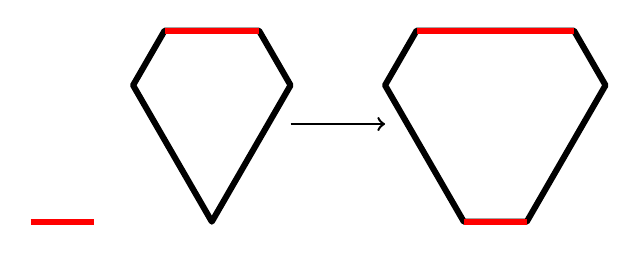
\begin{tikzpicture}[scale=2, line join=round]
  \def\L{1}
  \def\delta{0.6}
  \pgfmathsetmacro{\S}{\L-\delta}
  \pgfmathsetmacro{\xPent}{\S+0.75}
  \pgfmathsetmacro{\xHex}{\xPent+1.6}

  \draw[red, line width=2.2pt] (0,0) -- (\S,0);

  \node at (\S+0.30, {0.25*\L}) {$\boxplus$};

  \begin{scope}[xshift=\xPent cm]
    \path
      (0,0) coordinate (P0)
      -- ++(60:\L)       coordinate (P1)
      -- ++(120:\S)      coordinate (P2)
      -- ++(180:\delta)  coordinate (P3)
      -- ++(240:\S)      coordinate (P4);
    \draw[black, line width=2.2pt] (P0)--(P1)--(P2)--(P3)--(P4)--cycle;
    \draw[red,   line width=2.2pt] (P2)--(P3);
  \end{scope}

  \draw[->, line width=0.9pt] (\xPent+0.5, {0.62*\L}) -- (\xHex-0.5, {0.62*\L});

  \begin{scope}[xshift=\xHex cm]
    \path
      (0,0) coordinate (A)
      -- ++(0:\S)   coordinate (B)
      -- ++(60:\L)  coordinate (C)
      -- ++(120:\S) coordinate (D)
      -- ++(180:\L) coordinate (E)
      -- ++(240:\S) coordinate (F);
    \draw[black, line width=2.2pt] (A)--(B)--(C)--(D)--(E)--(F)--cycle;
    \draw[red,   line width=2.2pt] (A)--(B);
    \draw[red,   line width=2.2pt] (D)--(E);
  \end{scope}
\end{tikzpicture}
\end{figure}

\begin{proof}
We show that (i) $\iff$ (ii) and (i) $\iff$ (iii).

Suppose every 2-face of Z is opposite-parallel. Then for every edge $e \in Z$ write $S_e$ as the shortest edge in the zone $\ca{E}_e$ of $e$. Now we can obtain a polytope $P_e$ by "deleting" length $S_e$ from every edge (see illustration above), which then gives $Z = S_e \boxplus P_e$, a minkowski sum. Suppose that every for every edge $e \in Z$, we can write $Z$ as $S_e \boxplus P_e$, where $S_e$ is some multiple of the edge and $P_e$ is the polytope associated with it. Then clearly from the minkowski sum every 2-face is opposite parallel.

Now assume every 2-face of a $d$-polytope $Z$ is already opposite parallel. Then in fact every $k$-face of $Z$ for $2\leq k \leq d$ is opposite parallel. We modify the argument in \cite[Thm.~1]{Shephard1967PolytopesCentrallySymmetricFaces}. Let $P$ be any given $d$-polytope in $\mathbb{R}^d$, and $R$ be any $r$-flat (i.e. dimension $r$ affine subspace of $\mathbb{R}^d$ passing through the origin $o$. Let $\pi_R$ denote orthogonal projection on to $R$, so that $\pi_R(P)$ is an $r$-polytope in $R$. Then since, for each $j$ satisfying $0 \le j \le r-1$, the $j$-faces of $\pi_R(P)$ are the images under $\pi_R$ of faces of $P$ whose dimension is at least $j$, we deduce the following: If $j$ and $r$ are given integers satisfying $2 \le j \le r \le d$, and if $P$ is a $d$-polytope with opposite parallel $j$-faces, then the $j$-faces of $\pi_R(P)$ are also opposite parallel. Since they are opposite-parallel, for each hyperplane $H^+$ in the normal fan $\ca{N}(Z)$ we get a parallel hyperplane $H^-$ in the opposite direction, and thus $\ca{N}(Z)$ is a hyperplane arrangement. Now assume that $\ca{N}(Z)$ is a hyperplane arrangement. Then immediately ever 2-face of $Z$ must be opposite-parallel, and thus we are done.

\smallskip
This is actually a generalization. Indeed if all the 2-faces of a polytope $P$ were centrally symmetric, $P$ would be a zonotope, but parallel opposite edges doesn't imply central symmetry. Consider the above 2-polytope. Combinatorial equivalence between generalized zonotopes and zonotopes follows from (iii). Alternatively, we can "normalize" the generalized zonotope by forcing every edge to be of equal length, and thus recover a zonotope. 
\end{proof}

\item If every projection of a polytope to $\mathbb{R}^3$ is a zonotope, then the polytope is a zonotope itself. 

Show that the projections to $\mathbb{R}^2$ are not good enough for this. 

(Witsenhausen~[568])

\begin{proof}
    We proceed by the contrapositive. Recall from earlier that if every 2-face of a polytope $P$ is a zonotope, then so is $P$ itself. Thus assume that $P$ is not a polytope, so there exists some 2-face $F \in P$ that is not a zonotope. We will show that we must be able to display this face through some projection to $\mathbb{R}^3$, which then would not be a zonotope in $\mathbb{R}^3$.

    First consider $\aff(F)$, the 2-dimensional affine hull of $F$. We take two vectors $f_1, f_2$ which span this space. Then, consider the normal cone $N_P(F)$, and take an inward normal vector "exclusive" to $F$ (so it is not also the inward normal vector of some larger face containing $F$). Equivalently, consider the set of all all facets $\{F_i\}$ containing $F$, and take a positive combination of their inward normal vectors $n_i$, as in $v = \sum_{i} \lambda_ix_i, \; \lambda_i > 0$. In this case we see that projection to the 3-dimensional subspace spanned by $f_1, f_2$ and $v$, the non-zonotopal face $F$ remains a face of the projected polytope, and thus we are done.

    For a counterexample for projections to $\mathbb{R}^2$, note that every projection of a octahedron is a zonotope. In fact, we can write the octahedron as $\conv(\pm e_1, \pm e_2, \pm e_3)$, and thus for any projection $\pi: \mathbb{R}^3 \to \mathbb{R}^2$ we obtain the zonotope $\boxplus_{i=1}^3 [\pi(-e_i), \pi(e_i)]$
\end{proof}

\item Interpret the deletion and the contraction of a vector in the configuration $V$ in terms of zonotopes. That is, describe how the zonotopes $Z(V\backslash v)$ and $Z(V/v)$ can be constructed geometrically.

\begin{solution}
    Deleting $\bi{v}$ from $V$ simply removes it. Thus $Z(V\setminus\bi{v})$ is just $\boxplus_{v \in V \setminus\bi{v}}[0,v]$, the minkowski sum without the removed vector. Contracting by $\bi{v}$ in $V$ both removes it and projects the rest of the vectors in $V/\bi{v}$ to their orthogonal (to $\bi{v}$) component. Thus $Z(V/\bi{v}) = \pi(Z(V\setminus \bi{v}))$, where $\pi: \mathbb{R}^d \to \mathbb{R}^{d-1}, \; \pi(\bi{w} + t\bi{v}) = \bi{w}$ for $t \in \mathbb{R}$ and $\bi{w} \cdot \bi{v} = 0$
\end{solution}

\item Let $Z(V)$ be the zonotope generated by a configuration $V \in \mathbb{R}^{d\times n}$ which spans $\mathbb{R}^d$. Let $G \in (\mathbb{R}^*)^{(n-d)\times n}$ be the dual vector configuration.

\begin{enumerate}[label=(\roman*)]
\item How can the combinatorics of the zonotope $Z(V)$ be read off from the configuration $G$?
\item Use this to describe the zonotopes with $n \le d+2$ zones.
\item Describe the relation between the zonotope $Z(V)$ and its \emph{associated zonotope} $Z(G)\subseteq (\mathbb{R}^{n-d})^*$.
\end{enumerate}
(This was developed by McMullen~[392].)

\begin{solution}
Recall that (identifying $\mathbb{R}^n$ with $(\mathbb{R}^n)^*$ in the natural way) the dual configuration $G \in \mathbb{R}^{n \times (n-d)}$ corresponds to $\ker(V)$, when seeing $V$ as a map $V: \mathbb{R}^n \to \mathbb{R}^d$.

\begin{enumerate}[label=(\roman*)]
    \item For a column vector $g_i$ of $G$, its support $\supp(g_i)$ corresponds to a linear dependence amongst the projected unit vectors $\pi(e_i)$ (equiv. $v_i$, the $i$th column of $V$) for all the indices $i \in \supp(g_i)$. We have $Z(V) = \boxplus_{i=1}^n [0,v_i]$, and we know that there is a bijection between congruent faces of $Z(P)$ to a "flat" in $V$, which is a set of vectors $\{v_i\}_{i \in I}$ for which every other vector in $V$ is linearly independent with. Since the dual matrix $G = \ker(V)$ contains all the sufficient information, we can simply read each face

    \item We split into cases, by $n-d$

    Case 1: $n-d = 0$. Then $Z(V)$ is combinatorially equivalent (in fact isomorphic via an affine coordinate change) to the $n$-cube.

    Case 2: $n-d = 1$. Since $V$ spans $\mathbb{R}^d$, let the first $d$ vectors be $e_1, ..., e_d$ the unit vectors, and there are $d$ choices for the $d+1$'th vector $v$, seen by $1 \leq |\supp(v)| \leq d$. In particular, if $|\supp(v)| = 1$ then we obtain the $d$-cube again, if $|\supp(v)| = 2$ we obtain $\pyr^{d-2}(\textup{hexagon})$ (this is the only instance a non-square 2-face shows up), and if $\supp(v)| = d$ we have $f_i = \binom{d+1}{i}$ except when $f_d = 1$. The general count for some arbitrary $|\supp(v)|$ follows similarly.

    Case 3: $n-d = 2$. Follows similarly. Just use the criterion described in part (i).

    \item Let $\ca{M}(V)$ be the oriented matroid for the zonotope $Z(V)$. Then $Z(G)$ is the zonotope corresponding to the dual oriented matroid $\ca{M}(V)^*$
\end{enumerate}
\end{solution}

\item Assume that $x,y \in \mathbb{R}^d$ are given. Give an explicit formula for some small enough $\varepsilon>0$ such that
\[
\operatorname{sign}(x+\varepsilon y)=\operatorname{sign}(x)\circ \operatorname{sign}(y).
\]

\begin{solution}
    It suffices to guarantee that if $\sign(x_i) \neq \sign(y_i)$, then $\sign(x_i+\varepsilon y_i) = \sign(x_i)$. For this simply choose $0<\varepsilon < |\frac{x_i}{y_i}|$ for all $i$ where $x_i, y_i \neq 0$. 
\end{solution}

\item Let $\mathcal{V}^* \subset \{+,-,0\}^n$ be a system of sign vectors.
\begin{enumerate}[label=(\roman*)]
\item Assuming that (V0): $\mathbf{0}\in \mathcal{V}^*$ holds, show that the axioms (V1) and (V2) together are equivalent to the axiom
\[
\text{(V2'):\quad } \textsc{u},\textsc{v} \in \mathcal{V}^* \;\Longrightarrow\; \textsc{u}\circ(-\textsc{v})\in \mathcal{V}^*.
\]

\item Consider any affine arrangement of $n$ hyperplanes in which a positive side has been chosen for each of the hyperplanes. Show how a sign vector is associated with every face of the arrangement, and the resulting collection of sign vectors satisfies (V2$^\prime$) and (V3), but not in general (V0) and (V1).

\item Show that not every sign vector system satisfying (V2$^\prime$) and (V3) corresponds to an affine arrangement, even if we admit topologically deformed arrangements (``pseudoarrangements'').

(The characterization of the sign vector systems of affine oriented matroids was a difficult combinatorial problem, recently solved by Karlander [316].)
\end{enumerate}

\begin{proof}
\begin{enumerate}[label=(\roman*)]
    \item We first show (V1), (V2) $\implies$ (V2'). Since $\textsc{v} \in \ca{V}^*$, then by (V1) $-\textsc{v} \in \ca{V}^*$. By (V2) we have that $\textsc{u} \circ (-\textsc{v}) \in \ca{V}^*$, as desired. Conversely assume $(V2')$, and notice that $\textbf{0} \circ (-\textsc{u}) = -\textsc{u} \in \ca{V}^*$, so we recover (V1). Then, we have $\textsc{u} \circ -(-\textsc{v}) = \textsc{u} \circ \textsc{v} \in \ca{V}^*$, so we recover (V2).

    \item The sign vector assignment is naturally induced by choosing a positive side for every hyperplane, and if the face is contained within a hyperplane then that component is $0$. Notice that (V2') is simply "pushing $\textsc{u}$ out of the hyperplanes away from \textsc{v}." This can be made concrete by seeing that the indices not in the support of a vector are exactly the hyperplanes which it is contained in. Then, 

    \ermactually{fill this in}

    Now (V0) is generally not satisfied because we need there to be a common point of intersection of all hyperplanes for $\textbf{0} \in \ca{V}^*$. Then it follows that in general (V1) is not satisfied either.

    \item Consider any arrangement of 2 hyperplanes in $\mathbb{R}^2$. Even if we allow pseudoarrangements, there must be a point of intersection between the two hyperplanes, corresponding to $\textbf{0}$, which there need not be in a configuration. For example, consider the set $\{+-, -+, +0, -0, 0+, 0-\}$.
    
\end{enumerate}
\end{proof}

\item Let $D=(V,A)$ be a directed graph with $n$ arcs, $A=\{a_1,\ldots,a_n\}$. With every subset $U\subseteq V$ of its vertex set, associate a sign vector $\delta(U)\in\{+,-,0\}^n$, the ``directed cut'' of $U$, where $\delta(U)_i=+$ if $a_i$ is an arc that leaves the set $U$; $\delta(U)_i=-$ if $a_i$ enters the set $U$; and $\delta(U)_i=0$ otherwise:
\[
\delta(U)_i=
\begin{cases}
+ & \text{if } \operatorname{tail}(a_i)\in U \text{ and } \operatorname{head}(a_i)\notin U,\\
- & \text{if } \operatorname{tail}(a_i)\notin U \text{ and } \operatorname{head}(a_i)\in U,\\
0 & \text{if } \operatorname{tail}(a_i)\text{ and}\operatorname{head}(a_i)\text{ are both in }U \text{ or both not in }U.
\end{cases}
\]

Show that the family $\mathcal{V}^*:=\{\delta(U):U\subseteq V\}$ is an oriented matroid. What is its rank? 

What is the relation to the oriented matroid associated with such a digraph according to Exercise 6.3?

\begin{proof}
We show that $\ca{V}^*$ is an oriented matroid by checking the covector axioms. Taking $U = \varnothing$, we obtain $\textbf{0}$. Clearly $-\delta(U)$ is just $\delta([n]\setminus U)$. However, $\delta(U) \circ \delta(U')$ can correspond to no $\delta(U'')$ for all $U'' \subseteq V$. As we understand it this exercise is wrong, but this is probably a misinterpretation.
\end{proof}

\item Show directly from the axioms in Definition 7.21 that every oriented matroid of rank $r\le 2$ (that is, an oriented matroid $\mathcal{V}^*\subseteq\{+,-,0\}^n$ that does not contain a chain $0<X<X'<X''$) is realizable.

\begin{proof}
    We show that for a rank $\leq 2$ oriented matroid we can create a hyperplane arrangement with positive sides chosen that realizes it. To do this we simply consider a fan of lines in $\mathbb{R}^2$ which all pass through the origin. If two indices $i$ and $j$ agree in sign (i.e. $\textsc{u}_i = \textsc{u}_j$) for every covector \textsc{u}, then they correspond to parallel lines, and if they differ (but equal $0$ together) then they are antiparallel lines. We can simplify the oriented matroid by deleting these elements. The simplified oriented matroid is necessarily uniform, since every possible 2-dependency was removed in simplification (and there are no 3-independencies). This means we can simply draw the $n$ hyperplanes (say, evenly angled), arrange the $2n$ elements not containing $0$ into a cycle where each step one sign is flipped, and place them in the $2n$ regions of $\mathbb{R}^2$ created by the hyperplanes. Now put the parallel and antiparallel lines back in and thus we are done.
\end{proof}

\item Show the following theorem. Let $\mathcal{V}^*,C^*\subseteq\{+,-,0\}^n$ be sign vector systems such that $C^*$ is the collection of sign vectors of minimal nonempty support in $\mathcal{V}^*$, \[
C^*=\operatorname{MIN}(\mathcal{V}^*),
\]
while $\mathcal{V}^*$ is the collection of all conformal products of sign vectors in $C^*$, \[
\mathcal{V}^*=\{\,0\circ \textsc{v}_1\circ\cdots\circ \textsc{v}_k : k\ge 0,\ \textsc{v}_i\in C^* \text{ for } i=1,2,\ldots,k\,\}.
\]
Then $\mathcal{V}^*$ is the covector set of an oriented matroid (that is, it satisfies the axioms of Definition 7.21) if and only if $C^*$ is the set of cocircuits of an oriented matroid, that is, if $C^*$ satisfies the following cocircuit axioms:

\begin{enumerate}
\item[(C0)] $\textbf{0}\notin C^*$ (``The zero vector is not a cocircuit'')
\item[(C1)] $\textsc{u}\in C^* \Longrightarrow -\textsc{u}\in C^*$ (``The negative of a cocircuit is always a cocircuit'')
\item[(C2)] $\textsc{u},\textsc{v}\in C^*,\ \operatorname{supp}(\textsc{u})\subseteq \operatorname{supp}(\textsc{v})\Longrightarrow \textsc{u}=\pm \textsc{v}$ (``Cocircuits have noncomparable supports'')
\item[(C3)] $\textsc{u},\textsc{v}\in C^*,\ \textsc{u}\ne -\textsc{v},\ j\in S(\textsc{u},\textsc{v})\Longrightarrow \exists \textsc{w}\in C^*,\, \textsc{w}'\in\{+,-,0\}^n:\ \textsc{w}\le \textsc{w}',\ $ and $\textsc{w}'$ eliminates $j$ between $\textsc{u}$ and $\textsc{v}$ (``The set of cocircuits admits elimination'')
\end{enumerate}

\begin{proof}
We first show that for a given set of covectors $\ca{V}^*$ satisfying the covector axioms, its cocircuit set $\ca{C}^*$ satisfies the cocircuit axioms. (C0) follows from definition ("minimal \textit{nonempty} support"), and (C1) follows from (V1). Now assume (C2) was false for a pair of vectors \textsc{u}, \textsc{v}, so that there exists some component $\textsc{u}_i = -\textsc{v}_i$. Then $i \in S(\textsc{u}, \textsc{v})$, and by (V3) there must be a covector \textsc{w} which eliminates $i$, and now $\supp(\textsc{w}) \subsetneq \supp(\textsc{v})$, so \textsc{v} was not a cocircuit. Now (C3) follows from (V3) and looking at the conformal product of \textsc{w}'.

Now assume a set of cocircuits $\ca{C}^*$ satisfying the cocircuit axioms have been given. We will show that, taking all possible conformal products, we obtain a set of covectors $\ca{V}^*$ that satisfy the covector axioms. Taking $k=0$ in the conformal product gives (V0). Now notice if $V = 0\circ \textsc{v}_1\circ\cdots\circ \textsc{v}_k$, then $-V = 0\circ (-\textsc{v}_1)\circ\cdots\circ (-\textsc{v}_k)$, which proves (V1). The composition of two covectors can be written as adjoining all components of the second conformal product that is also conformal to the first conformal product (note that for a conformal product/composition "$\circ$" becomes commutative). This proves (V2). For eliminating $j \in S(\textsc{u}, \textsc{v})$, we can one by one eliminate $j$ for each cocircuit in the conformal product of \textsc{u} and \textsc{v}, taking the conformal product of each of these no-longer cocircuits, and apply (C3) to find \textsc{w}. We can always do this without losing any components because there always exists a cocircuit \textsc{u} for a covector \textsc{v} and an index $i$, such that $\textsc{u} \leq \textsc{v}$ and $\textsc{u}_i = \textsc{v}_i$. This proves (V3), and thus we are done.
\end{proof}

\item Show that for any vector subspace $U\subseteq\mathbb{R}^n$, the set of minimal nonempty supports in $\mathcal{U}=\mathrm{SIGN}(U)$, given by \[
\operatorname{MIN}(\mathrm{SIGN}(U))
=\{\,u\in \mathrm{sign}(U)\setminus\{0\} : v\in \mathrm{sign}(U),\ \operatorname{supp}(v)\subset \operatorname{supp}(u)
\text{ implies } v=0\,\},
\]
is the set of cocircuits of an oriented matroid, that is, it satisfies the axioms of Exercise 7.12.

\begin{proof}
(C0) is immediately satisfied. (C1) is satisfied by the inverse property of a vector (sub)space. Now assume if for two vectors $\bi{u}, \bi{v} \in U$, we have that $\supp(\bi{u}) \subseteq \supp(\bi{v})$. Then under multiplication by a suitable constant $\lambda$ we can eliminate a component, such that $\supp(\lambda\bi{u} + \bi{v}) \subsetneq \supp(\bi{v})$, meaning $\bi{v}$ is not a cocircuit. This proves (C2). Now for (C3) we can easily obtain $\bi{w}'$ which eliminates $j \in S(\bi{u}, \bi{v})$ via the vector space axioms. Now we obtain the cocircuit $\bi{w}$ because the descending chain ordered by inclusion of support has a minimum element. Thus we are done.
\end{proof}

\item How can you test whether a given zonotopal tiling is the picture of an actual zonotope? Show that, essentially, one has to decide whether a certain polyhedron has nonempty interior, which can be solved as a linear programming problem, as in Exercise 5.2(i). 

So, is it true that the first figure in Section 7.5 represents the picture of a 3-dimensional zonotope?

\item Show that every nontrivial zonotopal tiling in $\mathbb{R}^2$ (a tiling of a centrally symmetric polygon by centrally symmetric polygons) has a simple vertex on the boundary, and also a simple vertex in the interior.

\begin{proof}
Assume by contradiction that every boundary vertex of a centrally symmetric polygon (i.e. 2-zonotope) $P$ is non-simple, then there must be at least one edge $e \notin P$ added to every vertex.
\end{proof}

\item Consider the following zonotopal tiling.

Show that it corresponds to an arrangement of $9$ pseudolines which is not stretchable, because it violates Desargues' theorem.

Show that the pseudoline arrangement of the following tiling is also not stretchable.

(The second configuration is closely related to Ringel's simple configuration of $9$ pseudolines; one only has to delete the line at infinity and perturb the arrangement there.

These drawings were produced by J\"urgen Richter-Gebert, using his postscript program described and listed in [457], which produces exceptionally nice pictures of zonotopal tilings.)

\item Consider the following simplicial arrangement of $16$ pseudolines from Gr\"unbaum [255, p.~44].

\begin{enumerate}[label=(\roman*)]
\item Show that it is not realizable.
\item Use it to construct a simple zonotopal tiling of a $12$-gon whose oriented matroid is not realizable.
\end{enumerate}

\item For every $d$-zonotope, the numbers $f_k$ of $k$-faces satisfy the relations
\[
f_{k-1} \ge \frac{k}{d-k+1}f_k \quad \text{for } 1 \le k \le d,
\]
and thus $f_k \le \begin{pmatrix} d \\ k \end{pmatrix} f_0$.

(This is given in terms of hyperplane arrangements and oriented matroids in Fukuda, Tamura \& Tokuyama [214, 213].)

\begin{proof}
Recall that for a zonotope $Z(V)$ of a vector configuration $V \subseteq \mathbb{R}^d$, a set of vectors $V'$ form a face if $V'$ is a flat. In fact, for a $k$ dimension $V'$, exactly $2^{|V| - |V'|}$ k-faces are formed by it. Let $W$ be a $k-1$-flat, 

\end{proof}

\item For any vector configuration $V=\{\bi{v}_1,\ldots,\bi{v}_n\}\subseteq \mathbb{R}^d$, prove the volume formula for its zonotope:
\[
\operatorname{vol}(Z(V)) \;=\; 2^d \cdot \sum_{1\le i_1<\cdots<i_d\le n}
\left|\det\left(\bi{v}_{i_1},\ldots,\bi{v}_{i_d}\right)\right|.
\]
For this, decompose the zonotope into parallelepipeds, whose volumes are given by determinants.

(McMullen, see Shephard [495, Sect.~5], from where we have also taken the illustration.)

\begin{proof}
Recall that geometrically, the determinant of a set of vectors gives the (signed) area of the parallelpiped formed by these vectors. For the zonotope $Z(V) = \boxplus_{i=1}^n [-\bi{v}_i, \bi{v}_i]$, we have $\operatorname{vol}(Z(V)) = 2^d\operatorname{vol}(Z(V)')$, where $Z(V)' = \boxplus_{i=1}^n [0, \bi{v}_i]$. We can tile $Z(V)'$ using its Minkowski summands (a cubical dissection, as Shephard calls them), meaning the smallest pieces $Z(V)'_I = \boxplus_{i \in I} [0,\bi{v}_i]$, which are exactly when $|I| = d$ and the vectors are linearly independent. It is easy to see that $\operatorname{vol}(Z(V)'_I) = |\det(\{\bi{v}_i\}_{i \in I})|$, and summing across all components gives the desired formula, keeping in mind that a set of dependent vectors have determinant $0$.
\end{proof}

\item * You can use the formula in the preceding exercise to compute the volume of a zonotope, but that is not very effective: the formula has
$\begin{pmatrix} n \\ d \end{pmatrix}$ terms, which may all be nonzero.

Is there a fast (polynomial) way to compute the volume of a zonotope?

(Answer: most probably not --- this is \#P-hard according to Dyer, Gritzmann \& Hufnagel [187].)

\end{enumerate}

\bigskip
\section{Shellability and the Upper Bound Theorem}

\begin{enumerate}
\setcounter{enumi}{-1}
\renewcommand{\labelenumi}{8.\arabic{enumi}}

\item Show that every polyhedral subdivision of a $2$-polytope is extendably shellable: We can start with an arbitrary $2$-face, and never get stuck. (This is classical, see Newman [422], but also [173] and [239].) Show that one cannot, however, prescribe the last $2$-face of a shelling.

\begin{proof}
Extend the polyhedral subdivision to allow for not necessarily convex 2-faces. Then notice that for any starting 2-face we can always pick the next face in the shelling order, which shares an edge with the starting face. Shellability follows by induction.

To see that the last 2-face cannot be prescribed, consider the following setup: clearly the middle trianglular face cannot be the last face of the shelling order.

\begin{figure}[h]
    \centering
    \includegraphics[width=0.3\linewidth]{images/triangles.png}
\end{figure}
\end{proof}

\item
\begin{enumerate}[label=(\roman*)]
\item Show that a set of facets of the $d$-cube determines a shellable subcomplex of $\partial C_d$ if and only if it contains no facets (is empty), or all facets, or if it contains at least one facet such that the opposite facet is not in the complex. Deduce that the boundary complexes of the $d$-cubes are extendably shellable.
\item Describe a shelling of the $d$-dimensional crosspolytope. Use it to compute the $f$-vector and the $h$-vector of the $d$-dimensional crosspolytope.
\item Given the $h$-vector of a simplicial polytope $P$, how can one derive the $h$-vector of the bipyramid $\mathrm{bipyr}(P)$?
\item Verify that the $d$-dimensional crosspolytopes $C_d^{\Delta}$ are extendably shellable for $d \le 4$. (Surprisingly, they are \emph{not} extendably shellable for $d \ge 12$, as proved by Hall [269]!)
\end{enumerate}

\begin{proof}
\begin{enumerate}[label=(\roman*)]
    \item The first two cases are immediate. Then, if a facet $F$ is in the set and its opposite facet is not, then $\dim(F \cap F') = d-2$ for any other facets $F'$ in the set. Now if a partial shelling order contains the opposite facet for every facet which it contains, it can only be empty or all of $\partial C_d$. Thus the boundary complexes of the $d$-cubes are extendably shellable

    \item Label each octant in $\mathbb{R}^d$ with a sign vector in $\{+, -\}^d \cong \{0, 1\}^d$. Notice that for the $d$ dimensional cross-polytope $C_d^\Delta$, there is exactly one facet per octant (move the barycenter of the cross polytope to \textbf{0}). Notice that each octant is adjacent to exactly $d$ others, seen by flipping the $i$'th entry for each $i \in [d]$. We can simply shell lexicographically (i.e. from \textbf{0} to \textbf{1}).

    Thus $|R_j|$ can simply be read off as the number of $1$'s in the sign vector for a corresponding facet. We have $|\{j: |R_j| = i\}| = \binom{d}{i}$, and we have for an index $i$, $|R_i|$ is simply the number of $1$'s in its binary expansion. Then we have
    \[f_{k-1} = \sum_{j} \binom{d-|R_j|}{k-|R_j|} = \sum_{i=0}^k \binom{d}{i}\binom{d-i}{k-i} = \binom{d}{k}2^k.\]
    and
    \[h_k = \sum_{i=0}^k (-1)^{k-i} \binom{d-i}{d-k}f_{i-1} = \sum_{i=0}^k (-1)^{k-i} \binom{d-i}{d-k}\binom{d}{i}2^i = \binom{d}{k}\sum_{i=0}^k (-1)^{k-i}\binom{k}{i}2^i = \binom{d}{k}.\]
    which we would have seen coming anyways.

    \item Apart from the obvious but boring computational route, notice that 
    \[h_i(\bipyr(P)) = h_i(P) + h_{i-1}(P).\]
    One can verify that computing the f-vector of $P$, then the f-vector of $\bipyr(P)$, and then computing the h-vector of $\bipyr(P)$ yields the same relation.

    \item Immediate for $d \leq 3$. Then for $C_4^\Delta$

    \ermactually{just don't be stupid}
\end{enumerate}
\end{proof}

\item Show that an ordering $F_1, F_2, \ldots, F_s$ of the facets of a pure simplicial complex is a shelling order if and only if for every $i \ge 1$, the facet $F_i$ contains a unique minimal face which is not contained in an earlier facet $F_j$ with $j<i$.

Show that the permutation $F_1,\ldots,F_t$ is a shelling of $\Delta$ if and only if $\Delta$ is partitionable with a partition such that
\[
R_i \subseteq F_j \quad \Longrightarrow \quad i \le j.
\]

\begin{proof}
Assume $F_1, \ldots, F_s$ is a shelling order of a pure simplicial complex. Assume by contradiction that for some $i \in [s]$ the facet $F_i$ does not contain a \textit{unique} minimal (by inclusion) face not contained previously, so then there must be two faces $f_1, f_2$ that are mutually incomparable and are either contained by or incomparable to every other new face in $F_i$. Clearly $f_1$ and $f_2$ cannot both be vertices, 
\end{proof}

\item * Is every $d$-diagram shellable? What can you say about the case $d=3$?
(For $d=2$ this is true, by Exercise 8.0. If you want a guess for $d \ge 3$, I'd vote for ``no,'' because of the rule of thumb, ``if Bruggesser--Mani doesn't shell it, then it isn't shellable.'')

\item * If a polytopal complex $C$ is shellable, but not necessarily simplicial, is it still true that its stars and links are shellable?
(Be careful: results of Pachner [433] show that the boundary of a shellable ball need not be shellable. The answer is ``yes'' for stars according to Coudurier [163], but it might still be ``no'' for the links.)

\item Show that for every vertex $v$ of a $d$-polytope $P$, there is a polytopal complex $C$ that subdivides the boundary complex of the vertex figure, $|C|=P/v$, and that is combinatorially equivalent to $\operatorname{link}(v,C)$.
(The face fan of the complex $C$ is a \emph{flattening} of the boundary complex of $P$ at the vertex $v$; see MacPherson [373].)

\begin{proof}
    Consider the star of a vertex $v \in P$. Take its star (i.e. all facets containing $v$) and project onto the "slicing" hyperplane, like a regular diagram of the star of $v$, obtained by taking a point beyond $v$. Notice that at this point the vertex figure is a subcomplex. Now remove all faces including $v$ (in a complex sense) and the remaining complex is (combinatorially equivalent to) the link of $v$ in $P$. Notice that the vertex figure remains a subcomplex, and it is easy to see that subdividing it by placing in the vertices not edge-adjacent to $v$ gives us the earlier polytopal complex. Lastly $|C| = P/v$ follows immediately when we take the cone at vertex $v$ (formed by taking the  and observe that it contains $P$ 
\end{proof}

\item If $C=\mathcal{C}(\partial P)$ is the boundary complex of a (nonsimplicial) polytope and $v$ is a vertex of $P$, then $\operatorname{link}(v,C)$ is shellable. To prove this, show that the links are isomorphic to the boundary complexes of polytopes.
(Hint: Use a point beyond $v$.)

\begin{proof}
    Follows by Exercise 8.5 and the fact that the boundary (complex) of a polytope is shellable. The point beyond $v$ is used in the proof of Exercise 8.5
\end{proof}

\item * What is the smallest possible number of vertices for a nonshellable triangulation of a $3$-polytope?
(Rudin [468] claims that one needs $14$ vertices if the complex is realizable as a simplicial geometric subdivision of a simplex. Is that true?)
How many vertices are needed for a simplicial, nonshellable $3$-sphere?

\item * Beat Lemma 8.6: is this the smallest pile of cubes that is not extendably shellable?

\item Every shelling $F_1,F_2,\ldots,F_s$ of the facets of a polytope $P$ also induces, for every facet $F_i$, an ordering of the facets of $F_i$. Namely, one can take facets of $F_i$ in the order in which they appear in the list
\[
F_1 \cap F_i,\, \ldots,\, F_{i-1}\cap F_i,\, F_{i+1}\cap F_i,\, \ldots,\, F_s \cap F_i.
\]
A shelling is \emph{perfect} if this ordering is a shelling order of the boundary of $F_i$, for all $i$. For example, shellings of simplicial polytopes are always perfect.
\begin{enumerate}[label=(\roman*)]
\item Show that Bruggesser--Mani shellings are not perfect in general.
\item Show that the $d$-cubes $C_d$ have perfect shellings, for all $d \ge 1$.
\item Show that all $3$-polytopes have perfect shellings.
\item Show that the polars of cyclic polytopes $C_d(n)^{\Delta}$ have perfect shellings.
\item * Does every polytope have a perfect shelling? (Kalai)
\end{enumerate}

\begin{proof}
\begin{enumerate}[label=(\roman*)]
\item Consider the prism of a trapezoid. The B-M shelling leaving from the smaller of the two parallel square faces does not give a perfect shelling order.

\item Leaving through a vertex gives the desired perfect shelling.

\item Shell using the "star", first at a given vertex, then the star of all shelled faces, going say counter-clockwise.

\item We know that cyclic polytopes have perfect shellings because they are simplicial. The shelling for $C_d(n)^\Delta$ is induced by this shelling, where the order of the facets $F \subseteq C_d(n)^\Delta$ correspond to the facets as vertices in the original shelling order. Precisely, let $F = \conv(V)$. When all vertices $\bi{v}_i \in V$ show up in the original shelling order (i.e. the corresponding facets $F_i \subseteq C_d(n))$, then it is shelled. Any order suffices for facets appearing together. 

\ermactually{i think this is not exactly right? i have yet to use the structure of cyclic polytopes: i think the important aspect is that they are neighborly...}

\item idk tbh
\end{enumerate}
\end{proof}

\item For a $d$-polytope $P$, show that the linear functions on $P^{\Delta}$ in general position really correspond to the Bruggesser--Mani line shellings of $P$.

If $P$ is simplicial, verify that under this correspondence the vertices $v_j$ of in-degree $k$ on $P^{\Delta}$ correspond to the facets with restriction set of size $|R_j|=d-k$.

In particular, the formula
\[
f_0^{\circ}=h_0^{\circ}+2h_1^{\circ}+4h_2^{\circ}+\cdots+2^k h_k^{\circ}+\cdots+2^d h_d^{\circ},
\]
which we used for the total number of faces of $P^\Delta$ in Section 3.4, amounts to the evaluation of $f(1)=h(2)$ for the polytope $P$. 

Using this, show that Kalai's ``good orientations'' on the graph $G(P^\Delta)$ are exactly the shelling orders for $\partial P$.

\item Prove the upper bound theorem for simple $d$-polytopes with $n$ facets. For this, consider a linear function $c\in (\mathbb{R}^d)^*$ in general position on a simple $d$-polytope $P\subseteq \mathbb{R}^d$ with $n$ facets. For $t\in \mathbb{R}$ define $h_k^\Delta(P,t)$ to be the number of vertices in $\{x\in P : cx \le t\}$ that are the highest point for $k$ different edges (as suggested by the previous exercise). 

By letting $t$ increase, show that for all $t\in \mathbb{R}$,
\[
(d-k)h_k^\Delta(P,t) + (k+1)h_{k+1}^\Delta(P,t)
= \sum_F h_k^\Delta(F,t)
\le n\,h_{k+1}^\Delta(P,t),
\]
where the sum is over all the $n$ facets of $P$, and the second inequality follows from consideration of a linear function $c$ for which the vertices of $F$ are smaller than all other vertices of $P$. Deduce from this that
\[
h_k^\Delta(P) \le
\begin{pmatrix}
n-k-1\\
d-k
\end{pmatrix},
\]
for $d\ge k \ge d-\left\lfloor \frac{d}{2}\right\rfloor$, and from this the upper bound theorem. (This is the ``dual proof'' of the upper bound theorem 8.23, from McMullen [389, Note added in proof].)

\item For a simple $d$-polytope $P\subseteq \mathbb{R}^d$ with $n$ vertices, a numbering of the vertices by $1,2,\dots,n$ is called \emph{completely unimodal} if every $k$-face ($2\le k\le d$) has a unique local minimum, that is, every face $F$ has only one vertex such that all its neighbors on $F$ get a larger number.
\begin{enumerate}[label=(\roman*)]
\item Show that the completely unimodal numberings of $P$ exactly correspond to the shelling orders of the (simplicial) polar polytope $P^\Delta$ (Williamson Hoke [566, Prop.~1]; see also [279]).
\item Show that if $P$ is the $d$-dimensional cube, then it suffices to assume that the numbering has a unique local minimum on every $2$-face (Hammer, Simeone, Liebling \& de Werra [270]; see [566, Prop.~2]).
\item Show that the $4$-cube has a numbering that is not completely unimodal, but for which every $k$-face with $k\ne 2$ has a unique local minimum.
\item Construct a simple $3$-polytope $P$ with a numbering such that every $2$-face has a unique local minimum, but there are two local minima on $P$. (Hint: First construct an acyclic orientation of a $3$-polytopal graph such that there are two sinks, but only one sink if one restricts to one of the facets.)
\end{enumerate}

\item Let $f=(1,23,47,52,38,12)$.
\begin{enumerate}[label=(\roman*)]
\item Is $f$ the $f$-vector of a simplicial complex?
\item Is $f$ the $f$-vector of a shellable complex?
\item Is $f$ the $f$-vector of a simplicial polytope?
\end{enumerate}

\begin{solution}
\begin{enumerate}[label=(\roman*)]
    \item We use the Kruskal-Katona theorem, which say that $f$ is the $f$-vector of a simplicial complex $\Delta_f$ if and only if $f_{-1} = 1$ and $f_{k-1} \geq \partial_{k+1}(f_k)$ for $0 \leq k \leq d-1$. Through a direct computation we see that these relations are all satisfied, so $f$ is indeed a valid $f$-vector for some simplicial complex. In fact, we can explicitly construct it: consider the following maximal faces
    \[\{12345, 12346, 12356, 12456, 13456, 23456, 12347, 12357, 12457, 13457, 23457, 12367, \]
    \[1238, 1248, 1348, 378, 478, 578, 678\}\]
    combined with all edges $\binom{[10]}{2}$ and two extra $\{1, 11\}, \{2, 11\}$, and leave the remaining vertices isolated. One can count that this gives the desired vector $f$.
    \item No. Using Stanley's trick, we compute its $h$-vector to be $h = (1, 18, -35, 39, -12, 1)$. Since it is negative, $\Delta_f$ cannot be shellable.
    \item We see that in the $h$-vector, $h_k \neq h_{d-k}$, which violates the Dehn-Sommerville relations, and thus this is not the $f$-vector for a simplicial polytope.
\end{enumerate}
\end{solution}

\item Show that $\partial_k(n)$ is a monotonically increasing function of $n$ (for fixed $k$). Characterize the values $n$ for which $\partial_k(n)=\partial_k(n+1)$.

\begin{remark}
    non-decreasing.
\end{remark}

\begin{proof}
Recall that for a binomial expansion of $n$ in the form of
\[n = \binom{a_k}{k} + \cdots + \binom{a_1}{1}\]
with $a_k > \ldots > a_1 \geq 0$, we have following definition
\[\partial_k(n+1) = \binom{a_k}{k-1} + \cdots + \binom{a_1}{0}\]

We induct on $k$. Notice that the claim is trivially true for $k=1$, and thus assume it is true up to $k-1$. Thus the only possibility that can cause trouble is if $a_{k}(n+1) = a_k(n) + 1$. This means that $n+1 = \binom{a_k + 1}{k}$. So it suffice to show that $\binom{a_k + 1}{k-1} \geq \binom{a_k}{k-1} + \cdots + \binom{a_1}{0}$. By induction it suffices to show that $\binom{a_k + 1}{k-1} - \binom{a_k}{k-1} \geq \binom{a_{k-1}+1}{k-2}$, which is true because $\binom{a_k + 1}{k-1} = \binom{a_k}{k-1} + \binom{a_k}{k-2}$, and by definition $a_k \geq a_{k+1}+1$. It also follows that the fixed values where $\partial_k(n)=\partial_k(n+1)$ is when for some $i$ we have $a_i(n+1) = a_i(n) + 1$, and $a_i(n) = a_{i-1}(n)+1$, as well as the trivial case $k=1$ for all nonnegative $n$.
\end{proof}

\item Characterize the $f$-vectors of connected simplicial complexes, as follows. 

The sequence $f=(1,f_0,f_1,f_2,\dots,f_d)$ is the $f$-vector of a connected simplicial complex if and only if it satisfies the conditions of the Kruskal--Katona Theorem 8.32 and the additional relation
\[
\partial^3(f_2) \le f_1 - f_0 + 1.
\]
(This is due to Bj\"orner [91].)

\begin{remark}
    Multiple simplicial complexes can correspond to the same $f$-vector. This claim only states that one of the realizations for a satisfactory $f$-vector need be connected.
\end{remark}

\begin{proof}
Recall that $\partial^k$ is the analogue for $\partial_k$ but with multi-binomnial coefficients (i.e. multichoose).

The Kruskal-Katona Theorem gives (biconditionally) that $f$ is the $f$-vector of a simplicial complex $\Delta_f$. So we prove that $\Delta_f$ is connected $\iff \partial^3(f_2) \le f_1 - f_0 + 1$. Notice it suffices to consider the 2D "layer" of $\Delta_f$, meaning simply $f_2, f_1, f_0$. Thus we can assume $\dim \Delta_f \leq 2$. Now if $f_2 = 0$ we see that $f_1 + 1 = f_0$, meaning we can realize the desired $f$-vector with a tree. It suffices to show that the equality case can be realized, and no larger, because a smaller .

\ermactually{this isnt super hard i think, just at a loss}
\end{proof}

\item* Characterize the $f$-vectors of pure simplicial complexes.
\begin{enumerate}[label=(\roman*)]
\item Start in low dimensions, with $2$-dimensional and $3$-dimensional simplicial complexes. Note that there are gaps: for example, a $2$-dimensional pure simplicial complex with $f_2=4$ faces has at least $f_1\ge 6$ edges, and at most $f_1\le 12$ edges --- but $f_1=7$ is impossible. (See Leck [351].)
\item In general, this is probably an intractable problem, since a complete answer would solve virtually all basic problems in design theory --- this observation may originally be due to Singhi \& Shrikhande [501, p.~67]; it is called ``trivial'' there. (See [67] for more on design theory.) As an example, show that the existence of a projective plane of order $d$ is equivalent to the existence of a pure simplicial complex (of dimension $d$) with
\[
f_0=d^2+d+1=f_d
\qquad\text{and}\qquad
f_1=
\begin{pmatrix}
f_0\\
2
\end{pmatrix}.
\]
(It is a notorious problem to show that such an object can exist only if $d$ is a power of a prime. The nonexistence is classical for $d=6$. It was only recently proved for $d=10$, by Lam, Thiel \& Swiercz and a CRAY 1A [348]. It is completely open for $d=12$. Don't try! Try!)
\end{enumerate}

\item For the standard octahedron $C_3^\Delta\subseteq \mathbb{R}^3$, find a shelling line $\ell\in \mathbb{R}^3$ that generates the shellings of Example 8.22. (Hint: Use Exercise 8.10.) Show that the facet ordering of the octahedron (labeled as in Example 8.22)
\[
123, 234, 345, 135, 246, 126, 156, 456,
\]
is a shelling order for the octahedron. Prove that, however, it is not a Bruggesser--Mani shelling for any realization of the octahedron. (Smilansky [504])

\begin{proof}
The B-M shelling as in Example 8.22 corresponds to a line leaving facet $123$ and returning to facet $456$. This can be achieved by simply picking the barycenter of facet $123$ as takeoff point and choosing the angle of the line such that the spaceship lands at the barycenter of $456$: its trajectory gives the desired shelling line.

The newly given order of facets is indeed a shelling order, and it corresponds to the B-M shelling if $\ell$ left through exactly the vertex $3$ and returned through $6$. However, such a line is not in general position and in general invalid as a shelling. No matter what realization of the octahedron we choose, exiting through a facet means shelling the adjacent facets (i.e. those sharing a ridge) first. However, the first four given facets of this shelling only mutually share a vertex, and thus it is not a B-M shelling.
\end{proof}

\item Derive
\[
f_{k-1}=\sum_{i=k}^{d}(-1)^{d-i}\begin{pmatrix} i \\ k \end{pmatrix}f_{i-1}\quad \text{for }k=0,1,\dots,d
\]
for the $f$-vector of a simplicial polytopes from the Dehn--Sommerville equations of Theorem 8.21. In particular, how does the ``obvious'' equation $2f_{d-2}=df_{d-1}$ follow from the Dehn--Sommerville equations?

\begin{solution}
Dehn-Sommerville
\end{solution}

\item Prove Stanley's trick: give a formula for the $(i,j)$-entry of Stanley's difference table, and show that the last row correctly computes the $h$-vector. Why are all the entries of the table nonnegative for a shellable complex?

\begin{proof}
Recall that $h(x) = f(x-1)$. Let $f = (f_{-1}, f_0, \ldots, f_d)$. Placing them along the right diagonal of the triangle, we see that the $j$'th element in the $i$'th row (where we start indexing both at $-1$, so $(-1,-1) = f_{-1} = 1)$ is equal to
\[f_{i,j} = \sum_{k=-1}^j (-1)^{j-k} \binom{i-k-1}{j-k} f_k\]
We can verify that
\[f_{i-1, j} - f_{i-1, j-1} = f_{i,j}\]

In particular with $f = (f_{-1}, f_0, \ldots, f_d)$, we have $h_{j+1} = f_{d+1, j} = \sum_{k=-1}^j (-1)^{j-k} \binom{d+k}{j-k} f_k$. For a shellable complex, all the elements in this triangle are nonnegative because all $h_i$ are positive, and since we start with nonnegative entries there cannot be any negative entries (by a simple argument).
\end{proof}

\item \begin{enumerate}[label=(\roman*)]
\item Prove that for $0\le j\le k\le d$, one has
\[
\sum_{i=j}^{d}\begin{pmatrix} d-i \\ k-i \end{pmatrix}=\begin{pmatrix} d+1-j \\ d+1-k \end{pmatrix}.
\]
\item Prove directly that for $0\le j\le d<n$, we have
\[
\sum_{i=0}^{j}(-1)^{j-i}\begin{pmatrix} d-i \\ d-j \end{pmatrix}\begin{pmatrix} n \\ i \end{pmatrix}=\begin{pmatrix} n-d-1+j \\ j \end{pmatrix}.
\]
For this, verify that the equation is true for $d=j$ (by induction) and for $j=0$, and then use induction on $d$, where the left-hand side and the right-hand side satisfy the same simple recursion. (See [252, p.~149], and also [240, p.~169].) Use this to compute the $h$-vector for simplicial neighborly polytopes, directly from Definition 8.18.
\end{enumerate}

\begin{proof}
\begin{enumerate}[label=(\roman*)]
\item Notice $\binom{d-i}{k-i} = \binom{d-i}{d-k}$. Now send all variables $x \to d-x$ and thus we get 
\[\sum_{i = 0}^j \binom{i}{k} = \binom{j+1}{k+1}\]
which is just the hockey-stick identity.

\item We first assume $d=j$; the equation becomes 
\[\sum_{i=0}^d (-1)^{d-i}\binom{n}{i} = \binom{n-1}{d}\]
which is obvious by inducting on $n$. Now set $j=0$ and obtain the obvious $1=1$. Now we induct on $d$, but this follows immediately because of the Pascal identity $\binom{d}{r} = \binom{d-1}{r} + \binom{d-1}{r-1}$. The computation for the $h$-vector of simplicial neighborly polytopes as in Definition 8.18 follows immediately.

\end{enumerate}
\end{proof}

\item Use Exercise 2.20 to show that one need not consider unbounded polyhedra for the upper bound theorem, as follows. For every unbounded $d$-polyhedron $P$ with at least two vertices, there exists a $d$-polytope with the same number of facets, but with more vertices than $P$. What happens in the cases where $P$ has at most one vertex?

\begin{proof}
Simply place a vertex in its lineality space and take the convex hull of all the vertices...

\ermactually{I have yet to do exercise 2.20 :opencry: I'll come back when i do it}
\end{proof}

\item Give natural bijections between 
\begin{itemize}
    \item the $k$-multisets with elements from $[n]$,
    \item the monomials of degree $k$ in the variables, $x_1,x_2,\dots,x_n$.
    \item and vectors $z\in \mathbb{N}_0^n$ with $\mathds{1}z=k$
\end{itemize}
Show that under these bijections, inclusion of multisets corresponds to divisibility of monomials and to the componentwise ordering of vectors. Give three more proofs of
\[
\left(\!\!\begin{pmatrix} n \\ k \end{pmatrix}\!\!\right)=\begin{pmatrix} n+k-1 \\ k \end{pmatrix}.
\]
For example, \begin{enumerate}[label=(\roman*)]
\item Show that every $k$-multiset with elements in $[n]$ corresponds to a sequence like $\ast\mid\ast\ast\mid\ast\ast\ast\ast\mid$ with $n$ stars and $k-1$ bars, where the number of stars between the $i$th bar and the $(i-1)$st bar is the multiplicity of $i$ in the multiset. Then count the star-bar strings.
\item Use induction on $n$, and a basic identity for binomial coefficients.
\end{enumerate}
For inspiration, see also Stanley [517, Sect.~1.2].

\begin{proof}
A multiset $\{i_1, \ldots, i_k\}$ naturally corresponds to the monomial $x_{i_1} \cdot \ldots \cdot x_{i_k}$, which naturally corresponds to the vector $z = (\textup{\# of 1}, \ldots, \textup{\# of n})$. The claims follow immediately.

Now we show the binomial identity. A multiset of size $k$ from $[n]$ corresponds to $k$ stars which are the elements and $n-1$ bars serving as dividers which indicate where each group of elements belong. This bijection gives the desired equation. Alternative induct on $n$ and note that we have
\[\left(\!\!\begin{pmatrix} n+1 \\ k \end{pmatrix}\!\!\right) = \sum _{i=0}^k\left(\!\!\begin{pmatrix} n \\ i \end{pmatrix}\!\!\right) = \sum_{i=0}^k \binom{n+i-1}{i} = \frac{(k+1)\binom{k+n}{k+1}}{n} = \binom{n+k}{k}\]
and an explicit bijection can be constructed from $S \in \left(\!\!\begin{pmatrix} [n] \\ k \end{pmatrix}\!\!\right)$ to $S' \in \binom{[n+k-1]}{k}$ by adding $i$ to the $i$'th element.
\end{proof}

\item On the vertex set $[3n]=\{1,2,\dots,3n\}$, consider the pure complex of dimension $d=3n-4$ generated by the $n$ facets $[3n]\setminus\{3i-2,3i-1,3i\}$ for $i=1,\dots,n$. There are $3^n$ minimal nonfaces: the sets of cardinality $n$ that contain exactly one of $3i-2,3i-1,3i$ for each $i$. By comparing this complex to an $(n+1)$-neighborly one, show that we have
\[
f_{i-1}=\begin{pmatrix} 3n \\ i \end{pmatrix}\ \ \text{and}\ \ h_i=\begin{pmatrix} i+3 \\ 3 \end{pmatrix}\quad \text{for }i<n,
\]
\[
f_{n-1}=\begin{pmatrix} 3n \\ n \end{pmatrix}-3^n\qquad h_n=\begin{pmatrix} n+3 \\ 3 \end{pmatrix}-3^n,
\]
\[
f_n=\begin{pmatrix} 3n \\ n+1 \end{pmatrix}-n\cdot 3^n\qquad h_{n+1}=\begin{pmatrix} n+4 \\ 3 \end{pmatrix}+(n-4)3^n,
\]
so that for $n\ge 6$ we have $h_n<0$, and the upper bound condition of Lemma 8.26 is violated for $h_{n+1}$ (where $n+1\le \left\lfloor \frac{d}{2}\right\rfloor$) for a pure complex. (Wistuba \& Ziegler [567])



\item Show that the $k$-skeleta of $d$-polytopes are shellable polyhedral complexes.

\begin{enumerate}[label=(\roman*)]
\item Show that $r$-lex order defines a shelling order $F_1(k),F_2(k),\dots$ for the $(k-1)$-skeleton of the $d$-simplex, by directly verifying condition 8.1(ii$'$).
\item Show that in fact the $k$-skeleta of all shellable polyhedral complexes are shellable.
\item * Is the $(k-1)$-skeleton of every $d$-simplex extendably shellable? (This is the \emph{shelling extension conjecture}, due to Simon [500, Ch.~5]; the conjecture is known to be true for $k\le 3$, by Bj\"orner \& Eriksson [92], and for $k\ge d-1$, by Kalai.)
\end{enumerate}

\item Show the following weaker version of Macaulay's theorem, which estimates the $M$-sequence $h=(h_0,h_1,\dots,h_d)$ without using the subtle operator $\partial^k$. If $h_k=\begin{pmatrix} x \\ k \end{pmatrix}$ for some real $x\in \mathbb{R}$ and if $k\ge 1$, then $h_{k-1}\ge \begin{pmatrix} x-1 \\ k-1 \end{pmatrix}$. 

(Bj\"orner, Frankl \& Stanley [93, Thm.~3])

\item* What combinatorial conditions on a simplicial complex imply that $h_i \le \begin{pmatrix} n-d-1+i \\ i \end{pmatrix}$? (The result is known for shellable complexes, but only with algebraic tools, like Kalai's ``algebraic shifting.'' Is there a fully combinatorial rule that with every shellable complex would associate a multicomplex whose $f$-vector is the $h$-vector of the complex? Can one prove it for pure complexes satisfying the Dehn--Sommerville equations, like Eulerian complexes [324] [62]?)

\item Show that the maximal number of vertices of a $d$-polytope with $2d$ facets is larger than the number of vertices of the $d$-cube, for $d\ge 4$. For large $d$, the maximal number is roughly
\[
\begin{pmatrix}
3\left\lfloor \frac{d}{2}\right\rfloor\\
\left\lfloor \frac{d}{2}\right\rfloor
\end{pmatrix}
\approx
\left(\frac{27}{4}\right)^{\left\lfloor \frac{d}{2}\right\rfloor},
\]
considerably more than $2^d$.

\item Show that the $f$-vectors of general $3$-polytopes are exactly the vectors of the form
\[
f(P_3)=(1,4,6,4)+a(0,1,1,0)+b(0,0,1,1),
\]
with $2a\ge b\ge 0$, $2b\ge a\ge 0$, and the $f$-vectors of simplicial $3$-polytopes are given by $b=2a$, i.e.,
\[
f(P_3)=(1,4,6,4)+g_1(0,1,3,2),\qquad g_1\ge 0.
\]

\begin{proof}
Recall by Steinitz's theorem that the graph of every $3$-polytope is $3$-connected, meaning it contains a $K_4$ minor, which corresponds to a tetrahedron and exactly the $f$-vector $(1,4,6,4)$, giving $a,b \geq 0$. Now reversing the deletions and contractions, we see that a deletion or a contraction can correspond to removing a face and a edge, or a edge and a vertex, which is exactly what is described here. Following this observation, the fact that $2a \geq b$ corresponds exactly to the fact that each facet contains at least $3$ edges, and $2b \geq a$ comes from the fact that each vertex is contained in at least $3$ edges. Now if all the facets are triangles, i.e. the 3-polytope is simplicial, we obtain the equality $b=2a$. Notably we cannot simultaneously have $a=2b$, unless $a=b=0$, where we obtain the simplex tetrahedron. 
\end{proof}

\item* Characterize the $f$-vectors of $d$-polytopes.

(The $f$-vectors for $3$-polytopes were characterized by Steinitz [526]; see the previous exercise. This is a big unsolved research problem for every $d\ge 4$. See Ehrenborg [193] for a recent account. For $d=4$, much more is known. For example, the possible pairs $(f_i,f_j)$ have been characterized for all $i<j$ (see Bayer [59], Bayer \& Lee [63, Sect.~3.8], and H\"oppner \& Ziegler [278]). According to [578] the \emph{fatness} parameter $F(P):=\frac{f_1+f_2-20}{f_0+f_3-10}$ plays a crucial role: Can it be arbitrarily large? Polytopes with $F(P)$ arbitrarily close to $9$ were constructed in [579], with further analysis in [472].)

\item Prove Bj\"orner's Theorem 8.39. 

For the first half, you need a lemma that verifies the monotonicity of the rows of $M_d$, and shows that the peak lies between $j=\left\lfloor\frac{3(d-1)}{4}\right\rfloor$ and $j=\left\lfloor\frac{d}{2}\right\rfloor$. For the second half, you can use $g$-vectors of the form
\[
g=\bigl(1,g_1,\begin{pmatrix} g_1 \\ 2 \end{pmatrix},\begin{pmatrix} g_1 \\ 3 \end{pmatrix},\dots,\begin{pmatrix} g_1 \\ k \end{pmatrix},0,\dots,0\bigr),
\]
such that the $k$th row of $M_d$ peaks at $m_{kp}$. Now let $g_1$ get very large.

\item Let $P$ be a simplicial $d$-polytope $P$, and let $P'$ be obtained by a stellar subdivision (as defined in Exercise 3.0: erecting a ``pyramidal cap'' over a facet). Show that
\[
f(\partial P')=f(\partial P)+f(\partial\Delta_d)+f(\partial\Delta_{d-1})-2f(\Delta_{d-1}).
\]

\item Consider the polytopes $C_d(n)^{\langle r\rangle}$ obtained by $r$ stellar subdivisions from cyclic ones. Using the previous exercise, show that the $g$-vector of $C_d(n)^{\langle r\rangle}$ is given by $(1,g_1+r,g_2,\dots,g_{\left\lfloor d/2\right\rfloor})$, where $g_i=\begin{pmatrix} n+d-2+i \\ i \end{pmatrix}$ represents the $g$-vector of the cyclic polytope $C_d(n)$.

\item* Are the $f$-vectors of (general) polytopes unimodal for $d\le 7$? (Connected sums of the form $P\# P^4$ have unimodal $f$-vectors in dimension $\le 7$, see Bj\"orner [90, Sect.~3].) Similarly, what is the smallest number of vertices for a $d$-polytope with nonunimodal $f$-vector? (Eckhoff [188] has nonunimodal $f$-vectors for $8$-polytopes with $6375$ vertices and for $9$-polytopes with only $1393$ vertices (Example 8.41). Can you do with less? In the case of simplicial polytopes, Eckhoff proved $d_0=19$, but the smallest number of vertices is not known, either; here $f_0=1320$ is the current record, see Example 8.40.)

\item For simplicial $d$-polytopes, show that $f_k<f_{d-2-k}$ and $f_k\le f_{d-1-k}$, for $0\le k\le \left\lfloor \frac{d-3}{2}\right\rfloor$. (Bj\"orner [86,90])

\item* Does $f_0<f_1<f_2<\cdots<f_{\lfloor d/4\rfloor}$ hold for all $d$-polytopes?

\item* Every centrally symmetric $d$-polytope has at least $3^d$ proper faces. 

(This is known in the case of simplicial and of simple polytopes, proved by Stanley [518]. However, even to show that every simplicial centrally symmetric polytope has at least $2^d$ facets --- a fact first proved by Bárány \& Lovász [38] --- one knows of no simple, ``elementary'' argument. Centrally symmetric $d$-polytopes with exactly $3^d$ proper faces exist: take for example the $d$-cubes, and all the polytopes which one can construct from $k$-cubes by taking products and polars. Kalai [302] conjectures that this yields all the polytopes with exactly $3^d$ proper faces.)

\item* For every integer $k\ge 1$, is there an integer $f(k)$ such that every $d$-polytope with $d\ge f(k)$ has a $k$-face that is either a simplex, or combinatorially equivalent to a $k$-cube? 

For every integer $k\ge 1$, is there an integer $g(k)$ such that every $d$-polytope with $d\ge g(k)$ has a \emph{quotient} that is a $k$-simplex, that is, it has faces $G_1\subseteq G_2$ such that $[G_1,G_2]\cong L(\Delta_k)=B_k$ (that is, the $k$-simplex arises as an iterated vertex figure of a face; cf.\ Exercise 2.9)? 

(The first question is due to Gil Kalai [303], who even conjectures that ``in some sense'' a ``typical'' $k$-face of a ``typical'' simple $d$-polytope with $n$ facets will be combinatorially equivalent to the $k$-cube, if $d$ and $n-d$ are both large enough compared with $k$. In [303], Kalai proves that $f(2)$ is finite --- in fact, $f(2)=5$. The second question is due to Micha Perles [438], who remarks that $g(0)=0$, $g(1)=1$, $g(2)=3$ (by Euler's equation), and $g(3)\ge 5$ (from the $24$-cell).)

\item Investigate the face numbers of cubical $d$-polytopes. In particular, show the following:
\begin{enumerate}[label=(\roman*)]
\item Every $3$-dimensional cubical polytope has more vertices than facets (in fact, $f_2=f_0-2$).
\item If $P$ is a cubical zonotope with $n$ zones, then
\[
f_0 = 2\left(\begin{pmatrix} n-1 \\ 0 \end{pmatrix}+\begin{pmatrix} n-1 \\ 1 \end{pmatrix}+\cdots+\begin{pmatrix} n-1 \\ d-1 \end{pmatrix}\right),
\qquad
f_{d-1}=2\begin{pmatrix} n \\ d-1 \end{pmatrix}.
\]
In particular, $P$ has more vertices than facets for $d\ge 3$.
\item If $P$ is a cubical $d$-polytope, then $f_k(P)\ge f_k(C_d)$ holds for all $k$. (Blind \& Blind [102])
\item Study the possible $f$-vectors of $4$-dimensional cubical polytopes. In particular, they can have more facets than vertices. (Jockusch [291])
\item[(v)*] Does every cubical $d$-polytope with $d\ge 4$ have an even number of vertices? (For even $d$ this was shown by Blind \& Blind [104].)
\end{enumerate}

\item* Is every cubical polytope rational?

\item The \emph{twisted lexicographic ordering} on the facets of $C_d(n)$ is defined as follows. Consider facets $F=\{i_1,\dots,i_d\}$ and $G=\{j_1,\dots,j_d\}$, and let $k$ be the smallest index where they differ, $i_k\ne j_k$. Setting $i_0=j_0=0$, define that $F\prec' G$ holds either if $i_k<j_k$ and $i_{k-1}=j_{k-1}$ is even, or if $i_k>j_k$ and $i_{k-1}=j_{k-1}$ is odd. Otherwise we set $F\succ' G$.
\begin{enumerate}[label=(\roman*)]
\item Show that every facet is adjacent to the previous one.
\item Show that $\prec'$ is a shelling order for $C_d(n)$, if $d\le 4$.
\item Show that $\prec'$ is not a shelling order in general. (Hint: list the first $8$ facets in the ordering for $C_7(10)$.)
\end{enumerate}
(This linear ordering is from G\"artner, Henk \& Ziegler [219, Sect.~5], motivated by Klee's construction [325, Thm.~1.1] of a Hamilton cycle in the graph of $C_d(n)^\Delta$. Part (iii) was observed by Robert Hebble.)

\item* Show that for $n\ge 8$ the cyclic polytope $C_4(n)$ cannot be realized in such a way that it has a Bruggesser--Mani shelling for which every facet is adjacent to the previous one. Equivalently, the polar $C_4(n)^\Delta$ cannot be realized with a monotone path through all the vertices. (Indeed, Pfeifle [441] verified that for $8\le n\le 12$ there is no Hamilton path that would satisfy the known combinatorial conditions:
\begin{enumerate}[label=(\roman*)]
\item induce a unique sink on each face [566] and
\item satisfy the Holt--Klee condition [282] that there are $d$ vertex-disjoint graphs from source to sink in any orientation of the graph of a simple $d$-polytope that is induced by a linear function.
\end{enumerate}
Thus it is an entirely combinatorial problem to show that no such ordering on the vertices of $C_4(n)^\Delta$ exists for any $n\ge 8$. There is no dual-to-neighborly polytope of dimension $d=6$ with $n=9$ facets and a monotone path through all its $f_0(C_6(9)^\Delta)=30$ vertices [443].

Thus, in general $M(d,n)$ is smaller than the value $f_0(C_d(n)^\Delta)$ provided by the upper bound theorem. Compare Problem 3.11*.)

\item* It seems to be an open problem to show that all $f$-vectors of cyclic polytopes are unimodal. Are they?

\item For $n>d\ge 2$, a \emph{stacked polytope} $\mathrm{St}_d(n)$ is a simplicial $d$-polytope with $n$ vertices that is obtained by starting with a $d$-simplex and successively adding $n-d-1$ vertices ``beyond a facet.''
\begin{enumerate}[label=(\roman*)]
\item Show that every stacked polytope $\mathrm{St}_d(n)$ is a connected sum of $d$-simplices.
\item Show that every polytope that is combinatorially isomorphic to $\mathrm{St}_d(n)$ is a stacked polytope. (In the terminology of [459], this is since the gluing simplex is ``necessarily flat.'')
\item Compute the $f$-vector of $\mathrm{St}_d(n)$, and show that for each fixed $d\ge 2$, it grows linearly with $n$.
\item Show that for every $d\ge 3$, the number of combinatorial types of stacked polytopes $\mathrm{St}_d(n)$ grows exponentially with $n$.
\end{enumerate}
\end{enumerate}


\bigskip
\section{Fiber Polytopes, and Beyond}

\begin{enumerate}
\setcounter{enumi}{-1}
\renewcommand{\labelenumi}{9.\arabic{enumi}}
\item For which of the examples of polytopes discussed in Lecture 0 can we, by now, give complete combinatorial descriptions? Which of them are related by projections? Which can we represent as fiber polytopes associated with a projection of simpler polytopes?

\item Compute the fiber polytope for the projection in Example 9.3. For this, compute both the vertex coordinates, corresponding to the six coherent tight sections. (According to our discussion, you should get a hexagon!)

Also, compute the point in $\mathbb{R}^3$ which corresponds to the noncoherent tight section of Example 9.3. Does it lie in the relative interior of the fiber polytope?

Finally, use the methods described in this chapter to derive a description of the fiber polytope by equations and inequalities.

\item For the projection
\[
\pi : C_3^\Delta \longrightarrow [-2,+2], \qquad x \longmapsto 2x_1 + x_2,
\]
enumerate all the $\pi$-induced subdivisions, and identify the $\pi$-coherent ones among them. Draw the whole poset, and show how it ``retracts'' to the subset of $\pi$-coherent subdivisions.

Compute the fiber polytope, and describe the position in the fiber polytope of the points that correspond to noncoherent subdivisions.

\item For a polytope projection $\pi : P \longrightarrow Q$, let $\mathcal{F}$ be any $\pi$-induced subdivision. Show that for every linear function $c \in (\mathbb{R}^p)^{*}$ there is a relative coherent subdivision $\mathcal{G}^{c}$ with $\mathcal{G}^{c} \le \mathcal{F}$. (The construction can be done analogously to Definition 9.2.)

Show that if $c$ is generic, then $\mathcal{G}^{c}$ is tight. Conclude that the minimal elements of $\omega(P,Q)$ are exactly the tight subdivisions.

\item Given a monomial $m = x_1^{t_1}x_2^{t_2}\cdots x_d^{t_d}$, define its degree by
\[
\deg(m) := \begin{pmatrix} t_1 \\ \vdots \\ t_d \end{pmatrix} \in \mathbb{R}^d.
\]
For a polynomial in $d$ variables,
\[
f = \sum_i \alpha_i m_i \in \mathbb{R}[x_1,\ldots,x_d],
\]
for $\alpha_i \in \mathbb{R}$ and monomials $m_i$, define its \emph{Newton polytope} by
\[
\Newton(f) := \conv\{\deg(m_i) : \alpha_i \neq 0\}.
\]
\begin{enumerate}[label=(\roman*)]
\item Show that $\Newton(f\cdot g) = \Newton(f) + \Newton(g)$. From this, describe the Newton polytope $\Newton(f^k)$. What can you say about $\Newton(f+g)$, and about $\Newton(f+\epsilon g)$ for small enough $\epsilon > 0$?
\item Describe $\Newton(\det(x_{ij}))$, for the determinant of an $(n \times n)$-matrix, with $d=n^2$ different variables as entries.
\end{enumerate}

\item If $\pi : P \longrightarrow Q$ is a projection of polytopes, then the $\pi$-induced subdivisions of $Q$ only use vertices in the finite set $\pi(\vert(P))$, which need not all be vertices of $Q$.

Show that if $P=\Delta_p$ is a simplex, then all the regular $\pi$-induced subdivisions of $Q$ are $\pi$-coherent.

\item Let $\pi : P \longrightarrow Q$ be a projection of polytopes, where $P \subset \mathbb{R}^p$ is a polytope on $n$ vertices. Show that the fiber polytope $\Sigma(P,Q)$ can be constructed by projecting the secondary polytope of $P$:
\[
\Sigma(P,Q) = \pi(\Sigma(P)).
\]
(Billera \& Sturmfels [78])

\item Verify the formulas for the volume (area) and the barycenter of the $(n+1)$-gon
\[
C_2(n+1) = \conv\left\{\begin{pmatrix} i \\ i^2 \end{pmatrix} : i=0,1,2,\ldots,n\right\}.
\]
What about the volume and the barycenter of the general cyclic polytopes $C_d(n+1)$?

\item Let $P$ and $Q$ be polygons in the plane. Show that the fiber polytope of the projection
\[
P \times Q \longrightarrow P+Q
\]
from the product to the Minkowski sum has a fiber polytope that is isomorphic to $P+(-Q)$. What goes wrong here if $Q$ degenerates to a line segment?

\item Define the \emph{join} $P*Q$ of two polytopes to be the convex hull of $P$ and $Q$, if they are placed into affine subspaces of some $\mathbb{R}^d$ such that their affine hulls $\aff(P)$ and $\aff(Q)$ are skew.

Show that $P*Q$ is a polytope of dimension $\dim(P)+\dim(Q)+1$, and that up to affine equivalence the join does not depend on the choice of affine subspaces.

Show that the secondary polytope $\Sigma(P*Q)$ of the join is isomorphic to $\Sigma(P)\times \Sigma(Q)$.
(Dalbec [170])

\item Consider the projection $\pi : \mathbb{R}^n \longrightarrow \mathbb{R}$, $\Delta_{n-1} \longrightarrow [1,n]$ given by $e_i \longmapsto i$.

Show that the fiber polytope $\Sigma(\Delta_{n-1},[1,n])$ of this map is combinatorially equivalent to an $(n-2)$-cube. Is it in fact affinely isomorphic to $C_{n-2}$?
(Gelfand, Kapranov \& Zelevinsky [230, Example 7.3.A].)

\item Compute the secondary polytope of $\Delta_{n-1}\times \Delta_1$. For that first determine the dimension of the secondary polytope, then determine its set of vertices. Before you start to actually compute vertices, you should figure out the combinatorics of the polytope you get. (It is a good old friend!)

Also, study the secondary polytopes of $\Delta_{n-1}\times \Delta_{m-1}$.
(See Gelfand, Kapranov \& Zelevinsky [230, Examples 7.3.C,D]; The secondary polytopes of products of simplices are really complicated: see Babson \& Billera [32]!)

\item Show that if $Z$ is a $d$-zonotope with $n$ zones, then the fiber polytope of the canonical projection
\[
\pi : C_n \longrightarrow Z
\]
is a zonotope as well.
(Billera \& Sturmfels [78, Thm.\ 6.1])

Compute the fiber polytopes for the projections
\[
C_4 \longrightarrow P_2^8, \qquad C_5 \longrightarrow P_2^{10}, \qquad \text{and} \qquad C_6 \longrightarrow P_2^{12},
\]
where $P_2^{2i}$ denotes a centrally symmetric $2i$-gon. For the projection $C_6 \longrightarrow P_2^{12}$, the answer depends on the specific choice of a $12$-gon. Determine the (five) different $f$-vectors that occur in this case.
(Sturmfels [533])

\item If $P$ and $Q$ are disjoint polytopes in $\mathbb{R}^d$, show that the region between them can be triangulated without new vertices. That is, there exists a simplicial subdivision of $\conv(P \cup Q)$ whose vertex set is $\vert(P)\cup \vert(Q)$, and such that there are subcomplexes that triangulate $P$ and $Q$.

(Hint: Start with a convex function that is linear on $P$ and constant on $Q$, and use it to ``lift'' $Q$. Then take the convex hull, and perturb all the vertices. The result is due to Goodman \& Pach [233].)

\item For arbitrary polytopes $P \subseteq \mathbb{R}^p$ and $Q_1,Q_2 \subseteq \mathbb{R}^q$, show that
\[
\Phi(P,Q_1+Q_2) \supseteq \Phi(P,Q_1) + \Phi(P,Q_2).
\]
Show that equality does not hold in general.
(Rambau \& Ziegler [450])

\item Compute the mapping polytopes
\[
\Phi\left(\left(\Delta_p,\frac{1}{p}\right),\left(\Delta_q,\frac{1}{q}\right)\right),
\]
and describe them combinatorially.

\item What is a \emph{cofiber polytope}?

(This should be a polytope that is naturally associated to any inclusion of polytopes $P \hookrightarrow Q$.)
%%%%%%%%%%%%%%%%%%%%%%%%%%%%%%%%%%%%%%%%%%%%%%%%%%%%%%%%%%%%%%%%%%%%%%%%%%%%%%%%%%%%%%%%%%%%%%%%%%%%%%%%%%%%%%%%%%%%%%%%%%%%%%%%%%%%%%%%%%%%
\end{enumerate}

\pagebreak
\bibliographystyle{alpha}
\bibliography{bib}     
\end{document}